\documentclass[twoside]{book}

% Packages required by doxygen
\usepackage{fixltx2e}
\usepackage{calc}
\usepackage{doxygen}
\usepackage[export]{adjustbox} % also loads graphicx
\usepackage{graphicx}
\usepackage[utf8]{inputenc}
\usepackage{makeidx}
\usepackage{multicol}
\usepackage{multirow}
\PassOptionsToPackage{warn}{textcomp}
\usepackage{textcomp}
\usepackage[nointegrals]{wasysym}
\usepackage[table]{xcolor}

% Font selection
\usepackage[T1]{fontenc}
\usepackage[scaled=.90]{helvet}
\usepackage{courier}
\usepackage{amssymb}
\usepackage{sectsty}
\renewcommand{\familydefault}{\sfdefault}
\allsectionsfont{%
  \fontseries{bc}\selectfont%
  \color{darkgray}%
}
\renewcommand{\DoxyLabelFont}{%
  \fontseries{bc}\selectfont%
  \color{darkgray}%
}
\newcommand{\+}{\discretionary{\mbox{\scriptsize$\hookleftarrow$}}{}{}}

% Page & text layout
\usepackage{geometry}
\geometry{%
  a4paper,%
  top=2.5cm,%
  bottom=2.5cm,%
  left=2.5cm,%
  right=2.5cm%
}
\tolerance=750
\hfuzz=15pt
\hbadness=750
\setlength{\emergencystretch}{15pt}
\setlength{\parindent}{0cm}
\setlength{\parskip}{3ex plus 2ex minus 2ex}
\makeatletter
\renewcommand{\paragraph}{%
  \@startsection{paragraph}{4}{0ex}{-1.0ex}{1.0ex}{%
    \normalfont\normalsize\bfseries\SS@parafont%
  }%
}
\renewcommand{\subparagraph}{%
  \@startsection{subparagraph}{5}{0ex}{-1.0ex}{1.0ex}{%
    \normalfont\normalsize\bfseries\SS@subparafont%
  }%
}
\makeatother

% Headers & footers
\usepackage{fancyhdr}
\pagestyle{fancyplain}
\fancyhead[LE]{\fancyplain{}{\bfseries\thepage}}
\fancyhead[CE]{\fancyplain{}{}}
\fancyhead[RE]{\fancyplain{}{\bfseries\leftmark}}
\fancyhead[LO]{\fancyplain{}{\bfseries\rightmark}}
\fancyhead[CO]{\fancyplain{}{}}
\fancyhead[RO]{\fancyplain{}{\bfseries\thepage}}
\fancyfoot[LE]{\fancyplain{}{}}
\fancyfoot[CE]{\fancyplain{}{}}
\fancyfoot[RE]{\fancyplain{}{\bfseries\scriptsize Generated by Doxygen }}
\fancyfoot[LO]{\fancyplain{}{\bfseries\scriptsize Generated by Doxygen }}
\fancyfoot[CO]{\fancyplain{}{}}
\fancyfoot[RO]{\fancyplain{}{}}
\renewcommand{\footrulewidth}{0.4pt}
\renewcommand{\chaptermark}[1]{%
  \markboth{#1}{}%
}
\renewcommand{\sectionmark}[1]{%
  \markright{\thesection\ #1}%
}

% Indices & bibliography
\usepackage{natbib}
\usepackage[titles]{tocloft}
\setcounter{tocdepth}{3}
\setcounter{secnumdepth}{5}
\makeindex

% Hyperlinks (required, but should be loaded last)
\usepackage{ifpdf}
\ifpdf
  \usepackage[pdftex,pagebackref=true]{hyperref}
\else
  \usepackage[ps2pdf,pagebackref=true]{hyperref}
\fi
\hypersetup{%
  colorlinks=true,%
  linkcolor=blue,%
  citecolor=blue,%
  unicode%
}

% Custom commands
\newcommand{\clearemptydoublepage}{%
  \newpage{\pagestyle{empty}\cleardoublepage}%
}

\usepackage{caption}
\captionsetup{labelsep=space,justification=centering,font={bf},singlelinecheck=off,skip=4pt,position=top}

%===== C O N T E N T S =====

\begin{document}

% Titlepage & ToC
\hypersetup{pageanchor=false,
             bookmarksnumbered=true,
             pdfencoding=unicode
            }
\pagenumbering{alph}
\begin{titlepage}
\vspace*{7cm}
\begin{center}%
{\Large Chess \\[1ex]\large Version 1 }\\
\vspace*{1cm}
{\large Generated by Doxygen 1.8.14}\\
\end{center}
\end{titlepage}
\clearemptydoublepage
\pagenumbering{roman}
\tableofcontents
\clearemptydoublepage
\pagenumbering{arabic}
\hypersetup{pageanchor=true}

%--- Begin generated contents ---
\chapter{Namespace Index}
\section{Packages}
Here are the packages with brief descriptions (if available)\+:\begin{DoxyCompactList}
\item\contentsline{section}{\mbox{\hyperlink{namespacechess}{chess}} }{\pageref{namespacechess}}{}
\item\contentsline{section}{\mbox{\hyperlink{namespacechess_1_1command}{chess.\+command}} }{\pageref{namespacechess_1_1command}}{}
\item\contentsline{section}{\mbox{\hyperlink{namespacechess_1_1controllers}{chess.\+controllers}} }{\pageref{namespacechess_1_1controllers}}{}
\item\contentsline{section}{\mbox{\hyperlink{namespacechess_1_1main}{chess.\+main}} }{\pageref{namespacechess_1_1main}}{}
\item\contentsline{section}{\mbox{\hyperlink{namespacechess_1_1models}{chess.\+models}} }{\pageref{namespacechess_1_1models}}{}
\item\contentsline{section}{\mbox{\hyperlink{namespacechess_1_1models_1_1enums}{chess.\+models.\+enums}} }{\pageref{namespacechess_1_1models_1_1enums}}{}
\item\contentsline{section}{\mbox{\hyperlink{namespacechess_1_1models_1_1pieces}{chess.\+models.\+pieces}} }{\pageref{namespacechess_1_1models_1_1pieces}}{}
\end{DoxyCompactList}

\chapter{Hierarchical Index}
\section{Class Hierarchy}
This inheritance list is sorted roughly, but not completely, alphabetically\+:\begin{DoxyCompactList}
\item \contentsline{section}{chess.\+models.\+pieces.\+Advisor\+Test}{\pageref{classchess_1_1models_1_1pieces_1_1_advisor_test}}{}
\item \contentsline{section}{chess.\+models.\+pieces.\+Bishop\+Test}{\pageref{classchess_1_1models_1_1pieces_1_1_bishop_test}}{}
\item \contentsline{section}{chess.\+models.\+Board}{\pageref{classchess_1_1models_1_1_board}}{}
\item \contentsline{section}{chess.\+models.\+Board\+Test}{\pageref{classchess_1_1models_1_1_board_test}}{}
\item \contentsline{section}{chess.\+models.\+Chess\+Piece}{\pageref{classchess_1_1models_1_1_chess_piece}}{}
\begin{DoxyCompactList}
\item \contentsline{section}{chess.\+models.\+pieces.\+Advisor}{\pageref{classchess_1_1models_1_1pieces_1_1_advisor}}{}
\item \contentsline{section}{chess.\+models.\+pieces.\+Bishop}{\pageref{classchess_1_1models_1_1pieces_1_1_bishop}}{}
\item \contentsline{section}{chess.\+models.\+pieces.\+King}{\pageref{classchess_1_1models_1_1pieces_1_1_king}}{}
\item \contentsline{section}{chess.\+models.\+pieces.\+Knight}{\pageref{classchess_1_1models_1_1pieces_1_1_knight}}{}
\item \contentsline{section}{chess.\+models.\+pieces.\+Pawn}{\pageref{classchess_1_1models_1_1pieces_1_1_pawn}}{}
\item \contentsline{section}{chess.\+models.\+pieces.\+Queen}{\pageref{classchess_1_1models_1_1pieces_1_1_queen}}{}
\item \contentsline{section}{chess.\+models.\+pieces.\+Rook}{\pageref{classchess_1_1models_1_1pieces_1_1_rook}}{}
\item \contentsline{section}{chess.\+models.\+pieces.\+Soldier}{\pageref{classchess_1_1models_1_1pieces_1_1_soldier}}{}
\end{DoxyCompactList}
\item \contentsline{section}{chess.\+models.\+enums.\+Game\+Result}{\pageref{enumchess_1_1models_1_1enums_1_1_game_result}}{}
\item \contentsline{section}{chess.\+models.\+pieces.\+King\+Test}{\pageref{classchess_1_1models_1_1pieces_1_1_king_test}}{}
\item \contentsline{section}{chess.\+models.\+pieces.\+Knight\+Test}{\pageref{classchess_1_1models_1_1pieces_1_1_knight_test}}{}
\item \contentsline{section}{chess.\+models.\+enums.\+Move\+Result}{\pageref{enumchess_1_1models_1_1enums_1_1_move_result}}{}
\item \contentsline{section}{chess.\+models.\+Path}{\pageref{classchess_1_1models_1_1_path}}{}
\item \contentsline{section}{chess.\+models.\+Path\+Test}{\pageref{classchess_1_1models_1_1_path_test}}{}
\item \contentsline{section}{chess.\+models.\+pieces.\+Pawn\+Test}{\pageref{classchess_1_1models_1_1pieces_1_1_pawn_test}}{}
\item \contentsline{section}{chess.\+models.\+enums.\+Player}{\pageref{enumchess_1_1models_1_1enums_1_1_player}}{}
\item \contentsline{section}{chess.\+models.\+Position}{\pageref{classchess_1_1models_1_1_position}}{}
\item \contentsline{section}{chess.\+models.\+Position\+Test}{\pageref{classchess_1_1models_1_1_position_test}}{}
\item \contentsline{section}{chess.\+models.\+pieces.\+Queen\+Test}{\pageref{classchess_1_1models_1_1pieces_1_1_queen_test}}{}
\item \contentsline{section}{chess.\+models.\+pieces.\+Rook\+Test}{\pageref{classchess_1_1models_1_1pieces_1_1_rook_test}}{}
\item \contentsline{section}{chess.\+models.\+pieces.\+Soldier\+Test}{\pageref{classchess_1_1models_1_1pieces_1_1_soldier_test}}{}
\item Application\begin{DoxyCompactList}
\item \contentsline{section}{chess.\+controllers.\+Board\+Controller}{\pageref{classchess_1_1controllers_1_1_board_controller}}{}
\end{DoxyCompactList}
\end{DoxyCompactList}

\chapter{Class Index}
\section{Class List}
Here are the classes, structs, unions and interfaces with brief descriptions\+:\begin{DoxyCompactList}
\item\contentsline{section}{\mbox{\hyperlink{classchess_1_1models_1_1pieces_1_1_bishop}{chess.\+models.\+pieces.\+Bishop}} }{\pageref{classchess_1_1models_1_1pieces_1_1_bishop}}{}
\item\contentsline{section}{\mbox{\hyperlink{classchess_1_1pieces_1_1_bishop_test}{chess.\+pieces.\+Bishop\+Test}} }{\pageref{classchess_1_1pieces_1_1_bishop_test}}{}
\item\contentsline{section}{\mbox{\hyperlink{classchess_1_1models_1_1_board}{chess.\+models.\+Board}} }{\pageref{classchess_1_1models_1_1_board}}{}
\item\contentsline{section}{\mbox{\hyperlink{classchess_1_1controllers_1_1_board_controller}{chess.\+controllers.\+Board\+Controller}} }{\pageref{classchess_1_1controllers_1_1_board_controller}}{}
\item\contentsline{section}{\mbox{\hyperlink{classchess_1_1_board_test}{chess.\+Board\+Test}} }{\pageref{classchess_1_1_board_test}}{}
\item\contentsline{section}{\mbox{\hyperlink{classchess_1_1models_1_1_chess_piece}{chess.\+models.\+Chess\+Piece}} }{\pageref{classchess_1_1models_1_1_chess_piece}}{}
\item\contentsline{section}{\mbox{\hyperlink{classchess_1_1models_1_1pieces_1_1_crab}{chess.\+models.\+pieces.\+Crab}} }{\pageref{classchess_1_1models_1_1pieces_1_1_crab}}{}
\item\contentsline{section}{\mbox{\hyperlink{enumchess_1_1models_1_1enums_1_1_game_result}{chess.\+models.\+enums.\+Game\+Result}} }{\pageref{enumchess_1_1models_1_1enums_1_1_game_result}}{}
\item\contentsline{section}{\mbox{\hyperlink{classchess_1_1models_1_1pieces_1_1_king}{chess.\+models.\+pieces.\+King}} }{\pageref{classchess_1_1models_1_1pieces_1_1_king}}{}
\item\contentsline{section}{\mbox{\hyperlink{classchess_1_1pieces_1_1_king_test}{chess.\+pieces.\+King\+Test}} }{\pageref{classchess_1_1pieces_1_1_king_test}}{}
\item\contentsline{section}{\mbox{\hyperlink{classchess_1_1models_1_1pieces_1_1_knight}{chess.\+models.\+pieces.\+Knight}} }{\pageref{classchess_1_1models_1_1pieces_1_1_knight}}{}
\item\contentsline{section}{\mbox{\hyperlink{classchess_1_1pieces_1_1_knight_test}{chess.\+pieces.\+Knight\+Test}} }{\pageref{classchess_1_1pieces_1_1_knight_test}}{}
\item\contentsline{section}{\mbox{\hyperlink{enumchess_1_1models_1_1enums_1_1_move_result}{chess.\+models.\+enums.\+Move\+Result}} }{\pageref{enumchess_1_1models_1_1enums_1_1_move_result}}{}
\item\contentsline{section}{\mbox{\hyperlink{classchess_1_1models_1_1_path}{chess.\+models.\+Path}} }{\pageref{classchess_1_1models_1_1_path}}{}
\item\contentsline{section}{\mbox{\hyperlink{classchess_1_1models_1_1pieces_1_1_pawn}{chess.\+models.\+pieces.\+Pawn}} }{\pageref{classchess_1_1models_1_1pieces_1_1_pawn}}{}
\item\contentsline{section}{\mbox{\hyperlink{classchess_1_1pieces_1_1_pawn_test}{chess.\+pieces.\+Pawn\+Test}} }{\pageref{classchess_1_1pieces_1_1_pawn_test}}{}
\item\contentsline{section}{\mbox{\hyperlink{enumchess_1_1models_1_1enums_1_1_player}{chess.\+models.\+enums.\+Player}} }{\pageref{enumchess_1_1models_1_1enums_1_1_player}}{}
\item\contentsline{section}{\mbox{\hyperlink{classchess_1_1models_1_1_position}{chess.\+models.\+Position}} }{\pageref{classchess_1_1models_1_1_position}}{}
\item\contentsline{section}{\mbox{\hyperlink{classchess_1_1_position_test}{chess.\+Position\+Test}} }{\pageref{classchess_1_1_position_test}}{}
\item\contentsline{section}{\mbox{\hyperlink{classchess_1_1models_1_1pieces_1_1_queen}{chess.\+models.\+pieces.\+Queen}} }{\pageref{classchess_1_1models_1_1pieces_1_1_queen}}{}
\item\contentsline{section}{\mbox{\hyperlink{classchess_1_1pieces_1_1_queen_test}{chess.\+pieces.\+Queen\+Test}} }{\pageref{classchess_1_1pieces_1_1_queen_test}}{}
\item\contentsline{section}{\mbox{\hyperlink{classchess_1_1models_1_1pieces_1_1_rook}{chess.\+models.\+pieces.\+Rook}} }{\pageref{classchess_1_1models_1_1pieces_1_1_rook}}{}
\item\contentsline{section}{\mbox{\hyperlink{classchess_1_1pieces_1_1_rook_test}{chess.\+pieces.\+Rook\+Test}} }{\pageref{classchess_1_1pieces_1_1_rook_test}}{}
\item\contentsline{section}{\mbox{\hyperlink{classchess_1_1models_1_1pieces_1_1_straight}{chess.\+models.\+pieces.\+Straight}} }{\pageref{classchess_1_1models_1_1pieces_1_1_straight}}{}
\end{DoxyCompactList}

\chapter{File Index}
\section{File List}
Here is a list of all files with brief descriptions\+:\begin{DoxyCompactList}
\item\contentsline{section}{G\+:/\+Chess/src/main/java/chess/controllers/\mbox{\hyperlink{_board_controller_8java}{Board\+Controller.\+java}} }{\pageref{_board_controller_8java}}{}
\item\contentsline{section}{G\+:/\+Chess/src/main/java/chess/models/\mbox{\hyperlink{_board_8java}{Board.\+java}} }{\pageref{_board_8java}}{}
\item\contentsline{section}{G\+:/\+Chess/src/main/java/chess/models/\mbox{\hyperlink{_chess_piece_8java}{Chess\+Piece.\+java}} }{\pageref{_chess_piece_8java}}{}
\item\contentsline{section}{G\+:/\+Chess/src/main/java/chess/models/\mbox{\hyperlink{_path_8java}{Path.\+java}} }{\pageref{_path_8java}}{}
\item\contentsline{section}{G\+:/\+Chess/src/main/java/chess/models/\mbox{\hyperlink{_position_8java}{Position.\+java}} }{\pageref{_position_8java}}{}
\item\contentsline{section}{G\+:/\+Chess/src/main/java/chess/models/enums/\mbox{\hyperlink{_game_result_8java}{Game\+Result.\+java}} }{\pageref{_game_result_8java}}{}
\item\contentsline{section}{G\+:/\+Chess/src/main/java/chess/models/enums/\mbox{\hyperlink{_move_result_8java}{Move\+Result.\+java}} }{\pageref{_move_result_8java}}{}
\item\contentsline{section}{G\+:/\+Chess/src/main/java/chess/models/enums/\mbox{\hyperlink{_player_8java}{Player.\+java}} }{\pageref{_player_8java}}{}
\item\contentsline{section}{G\+:/\+Chess/src/main/java/chess/models/pieces/\mbox{\hyperlink{_bishop_8java}{Bishop.\+java}} }{\pageref{_bishop_8java}}{}
\item\contentsline{section}{G\+:/\+Chess/src/main/java/chess/models/pieces/\mbox{\hyperlink{_crab_8java}{Crab.\+java}} }{\pageref{_crab_8java}}{}
\item\contentsline{section}{G\+:/\+Chess/src/main/java/chess/models/pieces/\mbox{\hyperlink{_king_8java}{King.\+java}} }{\pageref{_king_8java}}{}
\item\contentsline{section}{G\+:/\+Chess/src/main/java/chess/models/pieces/\mbox{\hyperlink{_knight_8java}{Knight.\+java}} }{\pageref{_knight_8java}}{}
\item\contentsline{section}{G\+:/\+Chess/src/main/java/chess/models/pieces/\mbox{\hyperlink{_pawn_8java}{Pawn.\+java}} }{\pageref{_pawn_8java}}{}
\item\contentsline{section}{G\+:/\+Chess/src/main/java/chess/models/pieces/\mbox{\hyperlink{_queen_8java}{Queen.\+java}} }{\pageref{_queen_8java}}{}
\item\contentsline{section}{G\+:/\+Chess/src/main/java/chess/models/pieces/\mbox{\hyperlink{_rook_8java}{Rook.\+java}} }{\pageref{_rook_8java}}{}
\item\contentsline{section}{G\+:/\+Chess/src/main/java/chess/models/pieces/\mbox{\hyperlink{_straight_8java}{Straight.\+java}} }{\pageref{_straight_8java}}{}
\item\contentsline{section}{G\+:/\+Chess/src/test/java/chess/\mbox{\hyperlink{_board_test_8java}{Board\+Test.\+java}} }{\pageref{_board_test_8java}}{}
\item\contentsline{section}{G\+:/\+Chess/src/test/java/chess/\mbox{\hyperlink{_position_test_8java}{Position\+Test.\+java}} }{\pageref{_position_test_8java}}{}
\item\contentsline{section}{G\+:/\+Chess/src/test/java/chess/pieces/\mbox{\hyperlink{_bishop_test_8java}{Bishop\+Test.\+java}} }{\pageref{_bishop_test_8java}}{}
\item\contentsline{section}{G\+:/\+Chess/src/test/java/chess/pieces/\mbox{\hyperlink{_king_test_8java}{King\+Test.\+java}} }{\pageref{_king_test_8java}}{}
\item\contentsline{section}{G\+:/\+Chess/src/test/java/chess/pieces/\mbox{\hyperlink{_knight_test_8java}{Knight\+Test.\+java}} }{\pageref{_knight_test_8java}}{}
\item\contentsline{section}{G\+:/\+Chess/src/test/java/chess/pieces/\mbox{\hyperlink{_pawn_test_8java}{Pawn\+Test.\+java}} }{\pageref{_pawn_test_8java}}{}
\item\contentsline{section}{G\+:/\+Chess/src/test/java/chess/pieces/\mbox{\hyperlink{_queen_test_8java}{Queen\+Test.\+java}} }{\pageref{_queen_test_8java}}{}
\item\contentsline{section}{G\+:/\+Chess/src/test/java/chess/pieces/\mbox{\hyperlink{_rook_test_8java}{Rook\+Test.\+java}} }{\pageref{_rook_test_8java}}{}
\end{DoxyCompactList}

\chapter{Namespace Documentation}
\hypertarget{namespacechess}{}\section{Package chess}
\label{namespacechess}\index{chess@{chess}}
\subsection*{Packages}
\begin{DoxyCompactItemize}
\item 
package \mbox{\hyperlink{namespacechess_1_1controllers}{controllers}}
\item 
package \mbox{\hyperlink{namespacechess_1_1models}{models}}
\end{DoxyCompactItemize}

\hypertarget{namespacechess_1_1command}{}\section{Package chess.\+command}
\label{namespacechess_1_1command}\index{chess.\+command@{chess.\+command}}
\subsection*{Classes}
\begin{DoxyCompactItemize}
\item 
class \mbox{\hyperlink{classchess_1_1command_1_1_chess_move}{Chess\+Move}}
\item 
class \mbox{\hyperlink{classchess_1_1command_1_1_chess_move_command}{Chess\+Move\+Command}}
\item 
interface \mbox{\hyperlink{interfacechess_1_1command_1_1_command}{Command}}
\item 
class \mbox{\hyperlink{classchess_1_1command_1_1_request_chess_move}{Request\+Chess\+Move}}
\end{DoxyCompactItemize}

\hypertarget{namespacechess_1_1controllers}{}\section{Package chess.\+controllers}
\label{namespacechess_1_1controllers}\index{chess.\+controllers@{chess.\+controllers}}
\subsection*{Classes}
\begin{DoxyCompactItemize}
\item 
class \mbox{\hyperlink{classchess_1_1controllers_1_1_board_controller}{Board\+Controller}}
\end{DoxyCompactItemize}

\hypertarget{namespacechess_1_1main}{}\section{Package chess.\+main}
\label{namespacechess_1_1main}\index{chess.\+main@{chess.\+main}}
\subsection*{Classes}
\begin{DoxyCompactItemize}
\item 
class \mbox{\hyperlink{classchess_1_1main_1_1_main}{Main}}
\end{DoxyCompactItemize}

\hypertarget{namespacechess_1_1models}{}\section{Package chess.\+models}
\label{namespacechess_1_1models}\index{chess.\+models@{chess.\+models}}
\subsection*{Packages}
\begin{DoxyCompactItemize}
\item 
package \mbox{\hyperlink{namespacechess_1_1models_1_1enums}{enums}}
\item 
package \mbox{\hyperlink{namespacechess_1_1models_1_1pieces}{pieces}}
\end{DoxyCompactItemize}
\subsection*{Classes}
\begin{DoxyCompactItemize}
\item 
class \mbox{\hyperlink{classchess_1_1models_1_1_board}{Board}}
\item 
class \mbox{\hyperlink{classchess_1_1models_1_1_board_test}{Board\+Test}}
\item 
class \mbox{\hyperlink{classchess_1_1models_1_1_chess_piece}{Chess\+Piece}}
\item 
class \mbox{\hyperlink{classchess_1_1models_1_1_path}{Path}}
\item 
class \mbox{\hyperlink{classchess_1_1models_1_1_path_test}{Path\+Test}}
\item 
class \mbox{\hyperlink{classchess_1_1models_1_1_position}{Position}}
\item 
class \mbox{\hyperlink{classchess_1_1models_1_1_position_test}{Position\+Test}}
\end{DoxyCompactItemize}

\hypertarget{namespacechess_1_1models_1_1enums}{}\section{Package chess.\+models.\+enums}
\label{namespacechess_1_1models_1_1enums}\index{chess.\+models.\+enums@{chess.\+models.\+enums}}
\subsection*{Classes}
\begin{DoxyCompactItemize}
\item 
enum \mbox{\hyperlink{enumchess_1_1models_1_1enums_1_1_game_result}{Game\+Result}}
\item 
enum \mbox{\hyperlink{enumchess_1_1models_1_1enums_1_1_move_result}{Move\+Result}}
\item 
enum \mbox{\hyperlink{enumchess_1_1models_1_1enums_1_1_player}{Player}}
\end{DoxyCompactItemize}

\hypertarget{namespacechess_1_1models_1_1pieces}{}\section{Package chess.\+models.\+pieces}
\label{namespacechess_1_1models_1_1pieces}\index{chess.\+models.\+pieces@{chess.\+models.\+pieces}}
\subsection*{Classes}
\begin{DoxyCompactItemize}
\item 
class \mbox{\hyperlink{classchess_1_1models_1_1pieces_1_1_advisor}{Advisor}}
\item 
class \mbox{\hyperlink{classchess_1_1models_1_1pieces_1_1_advisor_test}{Advisor\+Test}}
\item 
class \mbox{\hyperlink{classchess_1_1models_1_1pieces_1_1_bishop}{Bishop}}
\item 
class \mbox{\hyperlink{classchess_1_1models_1_1pieces_1_1_bishop_test}{Bishop\+Test}}
\item 
class \mbox{\hyperlink{classchess_1_1models_1_1pieces_1_1_king}{King}}
\item 
class \mbox{\hyperlink{classchess_1_1models_1_1pieces_1_1_king_test}{King\+Test}}
\item 
class \mbox{\hyperlink{classchess_1_1models_1_1pieces_1_1_knight}{Knight}}
\item 
class \mbox{\hyperlink{classchess_1_1models_1_1pieces_1_1_knight_test}{Knight\+Test}}
\item 
class \mbox{\hyperlink{classchess_1_1models_1_1pieces_1_1_pawn}{Pawn}}
\item 
class \mbox{\hyperlink{classchess_1_1models_1_1pieces_1_1_pawn_test}{Pawn\+Test}}
\item 
class \mbox{\hyperlink{classchess_1_1models_1_1pieces_1_1_queen}{Queen}}
\item 
class \mbox{\hyperlink{classchess_1_1models_1_1pieces_1_1_queen_test}{Queen\+Test}}
\item 
class \mbox{\hyperlink{classchess_1_1models_1_1pieces_1_1_rook}{Rook}}
\item 
class \mbox{\hyperlink{classchess_1_1models_1_1pieces_1_1_rook_test}{Rook\+Test}}
\item 
class \mbox{\hyperlink{classchess_1_1models_1_1pieces_1_1_soldier}{Soldier}}
\item 
class \mbox{\hyperlink{classchess_1_1models_1_1pieces_1_1_soldier_test}{Soldier\+Test}}
\end{DoxyCompactItemize}

\chapter{Class Documentation}
\hypertarget{classchess_1_1models_1_1pieces_1_1_advisor}{}\section{chess.\+models.\+pieces.\+Advisor Class Reference}
\label{classchess_1_1models_1_1pieces_1_1_advisor}\index{chess.\+models.\+pieces.\+Advisor@{chess.\+models.\+pieces.\+Advisor}}
Inheritance diagram for chess.\+models.\+pieces.\+Advisor\+:\begin{figure}[H]
\begin{center}
\leavevmode
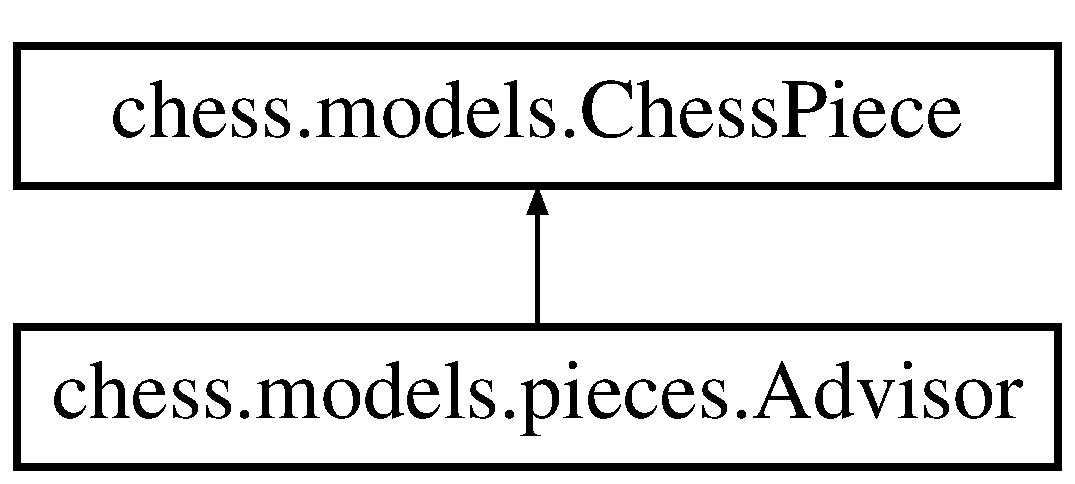
\includegraphics[height=2.000000cm]{classchess_1_1models_1_1pieces_1_1_advisor}
\end{center}
\end{figure}
\subsection*{Public Member Functions}
\begin{DoxyCompactItemize}
\item 
\mbox{\hyperlink{classchess_1_1models_1_1pieces_1_1_advisor_acad748f8b4188895b58996d0cef0a5d0}{Advisor}} (\mbox{\hyperlink{enumchess_1_1models_1_1enums_1_1_player}{Player}} \mbox{\hyperlink{classchess_1_1models_1_1_chess_piece_a3bcc8a24667318b5aab8c146adcc3eb7}{player}}, \mbox{\hyperlink{classchess_1_1models_1_1_position}{Position}} \mbox{\hyperlink{classchess_1_1models_1_1_chess_piece_a0e4f8616b75e548f269d3971846396f3}{position}})
\item 
\mbox{\hyperlink{enumchess_1_1models_1_1enums_1_1_move_result}{Move\+Result}} \mbox{\hyperlink{classchess_1_1models_1_1pieces_1_1_advisor_afd4015213fb9b97240f4235a9776f972}{is\+Legal\+Move}} (\mbox{\hyperlink{classchess_1_1models_1_1_position}{Position}} pos)
\item 
Set$<$ \mbox{\hyperlink{classchess_1_1models_1_1_position}{Position}} $>$ \mbox{\hyperlink{classchess_1_1models_1_1pieces_1_1_advisor_aec70114aea45fb0b4c102a81df30f60c}{get\+Nine\+Palaces}} ()
\end{DoxyCompactItemize}


\subsection{Detailed Description}
Custom chess piece\+: \mbox{\hyperlink{classchess_1_1models_1_1pieces_1_1_advisor}{Advisor}} 

\subsection{Constructor \& Destructor Documentation}
\mbox{\Hypertarget{classchess_1_1models_1_1pieces_1_1_advisor_acad748f8b4188895b58996d0cef0a5d0}\label{classchess_1_1models_1_1pieces_1_1_advisor_acad748f8b4188895b58996d0cef0a5d0}} 
\index{chess\+::models\+::pieces\+::\+Advisor@{chess\+::models\+::pieces\+::\+Advisor}!Advisor@{Advisor}}
\index{Advisor@{Advisor}!chess\+::models\+::pieces\+::\+Advisor@{chess\+::models\+::pieces\+::\+Advisor}}
\subsubsection{\texorpdfstring{Advisor()}{Advisor()}}
{\footnotesize\ttfamily chess.\+models.\+pieces.\+Advisor.\+Advisor (\begin{DoxyParamCaption}\item[{\mbox{\hyperlink{enumchess_1_1models_1_1enums_1_1_player}{Player}}}]{player,  }\item[{\mbox{\hyperlink{classchess_1_1models_1_1_position}{Position}}}]{position }\end{DoxyParamCaption})}

Constructor of \mbox{\hyperlink{classchess_1_1models_1_1_chess_piece}{Chess\+Piece}}


\begin{DoxyParams}{Parameters}
{\em player} & Belongs to which player \\
\hline
{\em position} & Initial position \\
\hline
\end{DoxyParams}


\subsection{Member Function Documentation}
\mbox{\Hypertarget{classchess_1_1models_1_1pieces_1_1_advisor_aec70114aea45fb0b4c102a81df30f60c}\label{classchess_1_1models_1_1pieces_1_1_advisor_aec70114aea45fb0b4c102a81df30f60c}} 
\index{chess\+::models\+::pieces\+::\+Advisor@{chess\+::models\+::pieces\+::\+Advisor}!get\+Nine\+Palaces@{get\+Nine\+Palaces}}
\index{get\+Nine\+Palaces@{get\+Nine\+Palaces}!chess\+::models\+::pieces\+::\+Advisor@{chess\+::models\+::pieces\+::\+Advisor}}
\subsubsection{\texorpdfstring{get\+Nine\+Palaces()}{getNinePalaces()}}
{\footnotesize\ttfamily Set$<$\mbox{\hyperlink{classchess_1_1models_1_1_position}{Position}}$>$ chess.\+models.\+pieces.\+Advisor.\+get\+Nine\+Palaces (\begin{DoxyParamCaption}{ }\end{DoxyParamCaption})}

\mbox{\Hypertarget{classchess_1_1models_1_1pieces_1_1_advisor_afd4015213fb9b97240f4235a9776f972}\label{classchess_1_1models_1_1pieces_1_1_advisor_afd4015213fb9b97240f4235a9776f972}} 
\index{chess\+::models\+::pieces\+::\+Advisor@{chess\+::models\+::pieces\+::\+Advisor}!is\+Legal\+Move@{is\+Legal\+Move}}
\index{is\+Legal\+Move@{is\+Legal\+Move}!chess\+::models\+::pieces\+::\+Advisor@{chess\+::models\+::pieces\+::\+Advisor}}
\subsubsection{\texorpdfstring{is\+Legal\+Move()}{isLegalMove()}}
{\footnotesize\ttfamily \mbox{\hyperlink{enumchess_1_1models_1_1enums_1_1_move_result}{Move\+Result}} chess.\+models.\+pieces.\+Advisor.\+is\+Legal\+Move (\begin{DoxyParamCaption}\item[{\mbox{\hyperlink{classchess_1_1models_1_1_position}{Position}}}]{pos }\end{DoxyParamCaption})}

Check if the movement is legal


\begin{DoxyParams}{Parameters}
{\em pos} & Destination position \\
\hline
\end{DoxyParams}
\begin{DoxyReturn}{Returns}
Move\+Result 
\end{DoxyReturn}


The documentation for this class was generated from the following file\+:\begin{DoxyCompactItemize}
\item 
G\+:/\+Chess/src/main/java/chess/models/pieces/\mbox{\hyperlink{_advisor_8java}{Advisor.\+java}}\end{DoxyCompactItemize}

\hypertarget{classchess_1_1models_1_1pieces_1_1_advisor_test}{}\section{chess.\+models.\+pieces.\+Advisor\+Test Class Reference}
\label{classchess_1_1models_1_1pieces_1_1_advisor_test}\index{chess.\+models.\+pieces.\+Advisor\+Test@{chess.\+models.\+pieces.\+Advisor\+Test}}
\subsection*{Public Member Functions}
\begin{DoxyCompactItemize}
\item 
void \mbox{\hyperlink{classchess_1_1models_1_1pieces_1_1_advisor_test_a865ff283ac107e64d2d27044ff25d02e}{is\+Legal\+Move}} ()
\item 
void \mbox{\hyperlink{classchess_1_1models_1_1pieces_1_1_advisor_test_a2ad02e014939d5e49e8cead14fd2eed5}{get\+Nine\+Palaces1}} ()
\item 
void \mbox{\hyperlink{classchess_1_1models_1_1pieces_1_1_advisor_test_aaa1de333725dbd1fb065c71272d9d555}{get\+Nine\+Palaces2}} ()
\item 
boolean \mbox{\hyperlink{classchess_1_1models_1_1pieces_1_1_advisor_test_a620e5937f1e6bbe806b60f364e103d19}{is\+Set\+Equals}} (Set$<$ \mbox{\hyperlink{classchess_1_1models_1_1_position}{Position}} $>$ expected\+Pos\+Set, Set$<$ \mbox{\hyperlink{classchess_1_1models_1_1_position}{Position}} $>$ actual\+Pos\+Set)
\end{DoxyCompactItemize}


\subsection{Member Function Documentation}
\mbox{\Hypertarget{classchess_1_1models_1_1pieces_1_1_advisor_test_a2ad02e014939d5e49e8cead14fd2eed5}\label{classchess_1_1models_1_1pieces_1_1_advisor_test_a2ad02e014939d5e49e8cead14fd2eed5}} 
\index{chess\+::models\+::pieces\+::\+Advisor\+Test@{chess\+::models\+::pieces\+::\+Advisor\+Test}!get\+Nine\+Palaces1@{get\+Nine\+Palaces1}}
\index{get\+Nine\+Palaces1@{get\+Nine\+Palaces1}!chess\+::models\+::pieces\+::\+Advisor\+Test@{chess\+::models\+::pieces\+::\+Advisor\+Test}}
\subsubsection{\texorpdfstring{get\+Nine\+Palaces1()}{getNinePalaces1()}}
{\footnotesize\ttfamily void chess.\+models.\+pieces.\+Advisor\+Test.\+get\+Nine\+Palaces1 (\begin{DoxyParamCaption}{ }\end{DoxyParamCaption})}

Method\+: get\+Nine\+Palaces(\+Position pos) \mbox{\Hypertarget{classchess_1_1models_1_1pieces_1_1_advisor_test_aaa1de333725dbd1fb065c71272d9d555}\label{classchess_1_1models_1_1pieces_1_1_advisor_test_aaa1de333725dbd1fb065c71272d9d555}} 
\index{chess\+::models\+::pieces\+::\+Advisor\+Test@{chess\+::models\+::pieces\+::\+Advisor\+Test}!get\+Nine\+Palaces2@{get\+Nine\+Palaces2}}
\index{get\+Nine\+Palaces2@{get\+Nine\+Palaces2}!chess\+::models\+::pieces\+::\+Advisor\+Test@{chess\+::models\+::pieces\+::\+Advisor\+Test}}
\subsubsection{\texorpdfstring{get\+Nine\+Palaces2()}{getNinePalaces2()}}
{\footnotesize\ttfamily void chess.\+models.\+pieces.\+Advisor\+Test.\+get\+Nine\+Palaces2 (\begin{DoxyParamCaption}{ }\end{DoxyParamCaption})}

\mbox{\Hypertarget{classchess_1_1models_1_1pieces_1_1_advisor_test_a865ff283ac107e64d2d27044ff25d02e}\label{classchess_1_1models_1_1pieces_1_1_advisor_test_a865ff283ac107e64d2d27044ff25d02e}} 
\index{chess\+::models\+::pieces\+::\+Advisor\+Test@{chess\+::models\+::pieces\+::\+Advisor\+Test}!is\+Legal\+Move@{is\+Legal\+Move}}
\index{is\+Legal\+Move@{is\+Legal\+Move}!chess\+::models\+::pieces\+::\+Advisor\+Test@{chess\+::models\+::pieces\+::\+Advisor\+Test}}
\subsubsection{\texorpdfstring{is\+Legal\+Move()}{isLegalMove()}}
{\footnotesize\ttfamily void chess.\+models.\+pieces.\+Advisor\+Test.\+is\+Legal\+Move (\begin{DoxyParamCaption}{ }\end{DoxyParamCaption})}

Method\+: is\+Legal\+Move(\+Position pos) \mbox{\Hypertarget{classchess_1_1models_1_1pieces_1_1_advisor_test_a620e5937f1e6bbe806b60f364e103d19}\label{classchess_1_1models_1_1pieces_1_1_advisor_test_a620e5937f1e6bbe806b60f364e103d19}} 
\index{chess\+::models\+::pieces\+::\+Advisor\+Test@{chess\+::models\+::pieces\+::\+Advisor\+Test}!is\+Set\+Equals@{is\+Set\+Equals}}
\index{is\+Set\+Equals@{is\+Set\+Equals}!chess\+::models\+::pieces\+::\+Advisor\+Test@{chess\+::models\+::pieces\+::\+Advisor\+Test}}
\subsubsection{\texorpdfstring{is\+Set\+Equals()}{isSetEquals()}}
{\footnotesize\ttfamily boolean chess.\+models.\+pieces.\+Advisor\+Test.\+is\+Set\+Equals (\begin{DoxyParamCaption}\item[{Set$<$ \mbox{\hyperlink{classchess_1_1models_1_1_position}{Position}} $>$}]{expected\+Pos\+Set,  }\item[{Set$<$ \mbox{\hyperlink{classchess_1_1models_1_1_position}{Position}} $>$}]{actual\+Pos\+Set }\end{DoxyParamCaption})}



The documentation for this class was generated from the following file\+:\begin{DoxyCompactItemize}
\item 
G\+:/\+Chess/src/test/java/chess/models/pieces/\mbox{\hyperlink{_advisor_test_8java}{Advisor\+Test.\+java}}\end{DoxyCompactItemize}

\hypertarget{classchess_1_1models_1_1pieces_1_1_bishop}{}\section{chess.\+models.\+pieces.\+Bishop Class Reference}
\label{classchess_1_1models_1_1pieces_1_1_bishop}\index{chess.\+models.\+pieces.\+Bishop@{chess.\+models.\+pieces.\+Bishop}}
Inheritance diagram for chess.\+models.\+pieces.\+Bishop\+:\begin{figure}[H]
\begin{center}
\leavevmode
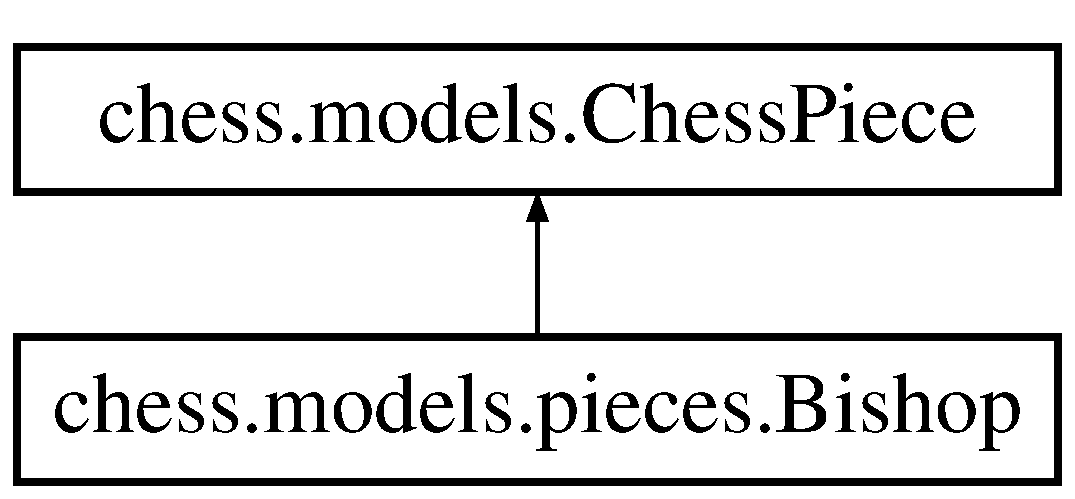
\includegraphics[height=2.000000cm]{classchess_1_1models_1_1pieces_1_1_bishop}
\end{center}
\end{figure}
\subsection*{Public Member Functions}
\begin{DoxyCompactItemize}
\item 
\mbox{\hyperlink{classchess_1_1models_1_1pieces_1_1_bishop_a9abc7cf53fde3e6ec5f8af6fbc7b005d}{Bishop}} (\mbox{\hyperlink{enumchess_1_1models_1_1enums_1_1_player}{Player}} \mbox{\hyperlink{classchess_1_1models_1_1_chess_piece_a3bcc8a24667318b5aab8c146adcc3eb7}{player}}, \mbox{\hyperlink{classchess_1_1models_1_1_position}{Position}} \mbox{\hyperlink{classchess_1_1models_1_1_chess_piece_a0e4f8616b75e548f269d3971846396f3}{position}})
\item 
\mbox{\hyperlink{enumchess_1_1models_1_1enums_1_1_move_result}{Move\+Result}} \mbox{\hyperlink{classchess_1_1models_1_1pieces_1_1_bishop_ae5a545cda22d44b4c4cbfeebab5c0853}{is\+Legal\+Move}} (\mbox{\hyperlink{classchess_1_1models_1_1_position}{Position}} pos)
\item 
String \mbox{\hyperlink{classchess_1_1models_1_1pieces_1_1_bishop_abbdf19ca47acb189eeaa49931eb2f30c}{to\+String}} ()
\end{DoxyCompactItemize}


\subsection{Detailed Description}
\mbox{\hyperlink{classchess_1_1models_1_1_chess_piece}{Chess\+Piece}} piece\+: \mbox{\hyperlink{classchess_1_1models_1_1pieces_1_1_bishop}{Bishop}} 

\subsection{Constructor \& Destructor Documentation}
\mbox{\Hypertarget{classchess_1_1models_1_1pieces_1_1_bishop_a9abc7cf53fde3e6ec5f8af6fbc7b005d}\label{classchess_1_1models_1_1pieces_1_1_bishop_a9abc7cf53fde3e6ec5f8af6fbc7b005d}} 
\index{chess\+::models\+::pieces\+::\+Bishop@{chess\+::models\+::pieces\+::\+Bishop}!Bishop@{Bishop}}
\index{Bishop@{Bishop}!chess\+::models\+::pieces\+::\+Bishop@{chess\+::models\+::pieces\+::\+Bishop}}
\subsubsection{\texorpdfstring{Bishop()}{Bishop()}}
{\footnotesize\ttfamily chess.\+models.\+pieces.\+Bishop.\+Bishop (\begin{DoxyParamCaption}\item[{\mbox{\hyperlink{enumchess_1_1models_1_1enums_1_1_player}{Player}}}]{player,  }\item[{\mbox{\hyperlink{classchess_1_1models_1_1_position}{Position}}}]{position }\end{DoxyParamCaption})}

Constructor of \mbox{\hyperlink{classchess_1_1models_1_1pieces_1_1_bishop}{Bishop}}


\begin{DoxyParams}{Parameters}
{\em player} & Belongs to which player \\
\hline
{\em position} & Initial position \\
\hline
\end{DoxyParams}


\subsection{Member Function Documentation}
\mbox{\Hypertarget{classchess_1_1models_1_1pieces_1_1_bishop_ae5a545cda22d44b4c4cbfeebab5c0853}\label{classchess_1_1models_1_1pieces_1_1_bishop_ae5a545cda22d44b4c4cbfeebab5c0853}} 
\index{chess\+::models\+::pieces\+::\+Bishop@{chess\+::models\+::pieces\+::\+Bishop}!is\+Legal\+Move@{is\+Legal\+Move}}
\index{is\+Legal\+Move@{is\+Legal\+Move}!chess\+::models\+::pieces\+::\+Bishop@{chess\+::models\+::pieces\+::\+Bishop}}
\subsubsection{\texorpdfstring{is\+Legal\+Move()}{isLegalMove()}}
{\footnotesize\ttfamily \mbox{\hyperlink{enumchess_1_1models_1_1enums_1_1_move_result}{Move\+Result}} chess.\+models.\+pieces.\+Bishop.\+is\+Legal\+Move (\begin{DoxyParamCaption}\item[{\mbox{\hyperlink{classchess_1_1models_1_1_position}{Position}}}]{pos }\end{DoxyParamCaption})}

Check if the movement is legal


\begin{DoxyParams}{Parameters}
{\em pos} & Destination position \\
\hline
\end{DoxyParams}
\begin{DoxyReturn}{Returns}
Move\+Result 
\end{DoxyReturn}
\mbox{\Hypertarget{classchess_1_1models_1_1pieces_1_1_bishop_abbdf19ca47acb189eeaa49931eb2f30c}\label{classchess_1_1models_1_1pieces_1_1_bishop_abbdf19ca47acb189eeaa49931eb2f30c}} 
\index{chess\+::models\+::pieces\+::\+Bishop@{chess\+::models\+::pieces\+::\+Bishop}!to\+String@{to\+String}}
\index{to\+String@{to\+String}!chess\+::models\+::pieces\+::\+Bishop@{chess\+::models\+::pieces\+::\+Bishop}}
\subsubsection{\texorpdfstring{to\+String()}{toString()}}
{\footnotesize\ttfamily String chess.\+models.\+pieces.\+Bishop.\+to\+String (\begin{DoxyParamCaption}{ }\end{DoxyParamCaption})}



The documentation for this class was generated from the following file\+:\begin{DoxyCompactItemize}
\item 
G\+:/\+Chess/src/main/java/chess/models/pieces/\mbox{\hyperlink{_bishop_8java}{Bishop.\+java}}\end{DoxyCompactItemize}

\hypertarget{classchess_1_1models_1_1pieces_1_1_bishop_test}{}\section{chess.\+models.\+pieces.\+Bishop\+Test Class Reference}
\label{classchess_1_1models_1_1pieces_1_1_bishop_test}\index{chess.\+models.\+pieces.\+Bishop\+Test@{chess.\+models.\+pieces.\+Bishop\+Test}}
\subsection*{Public Member Functions}
\begin{DoxyCompactItemize}
\item 
void \mbox{\hyperlink{classchess_1_1models_1_1pieces_1_1_bishop_test_a8da72169eb2ccd336e5a7a1535c246ac}{is\+Legal\+Move}} ()
\end{DoxyCompactItemize}


\subsection{Member Function Documentation}
\mbox{\Hypertarget{classchess_1_1models_1_1pieces_1_1_bishop_test_a8da72169eb2ccd336e5a7a1535c246ac}\label{classchess_1_1models_1_1pieces_1_1_bishop_test_a8da72169eb2ccd336e5a7a1535c246ac}} 
\index{chess\+::models\+::pieces\+::\+Bishop\+Test@{chess\+::models\+::pieces\+::\+Bishop\+Test}!is\+Legal\+Move@{is\+Legal\+Move}}
\index{is\+Legal\+Move@{is\+Legal\+Move}!chess\+::models\+::pieces\+::\+Bishop\+Test@{chess\+::models\+::pieces\+::\+Bishop\+Test}}
\subsubsection{\texorpdfstring{is\+Legal\+Move()}{isLegalMove()}}
{\footnotesize\ttfamily void chess.\+models.\+pieces.\+Bishop\+Test.\+is\+Legal\+Move (\begin{DoxyParamCaption}{ }\end{DoxyParamCaption})}



The documentation for this class was generated from the following file\+:\begin{DoxyCompactItemize}
\item 
src/test/java/chess/models/pieces/\mbox{\hyperlink{_bishop_test_8java}{Bishop\+Test.\+java}}\end{DoxyCompactItemize}

\hypertarget{classchess_1_1models_1_1_board}{}\section{chess.\+models.\+Board Class Reference}
\label{classchess_1_1models_1_1_board}\index{chess.\+models.\+Board@{chess.\+models.\+Board}}
\subsection*{Public Member Functions}
\begin{DoxyCompactItemize}
\item 
\mbox{\hyperlink{classchess_1_1models_1_1_board_a742cb1aaa3ec12625098a4ddf24fee19}{Board}} ()
\item 
\mbox{\hyperlink{enumchess_1_1models_1_1enums_1_1_move_result}{Move\+Result}} \mbox{\hyperlink{classchess_1_1models_1_1_board_a2514b6b830efc0aeeb2ba6f64aa033e2}{is\+Legal\+Move}} (\mbox{\hyperlink{classchess_1_1models_1_1_chess_piece}{Chess\+Piece}} chess\+Piece, \mbox{\hyperlink{classchess_1_1models_1_1_position}{Position}} pos)
\item 
boolean \mbox{\hyperlink{classchess_1_1models_1_1_board_a8ffee6403d98b5e5e68c0a2b73440100}{is\+Over\+Piece}} (\mbox{\hyperlink{classchess_1_1models_1_1_chess_piece}{Chess\+Piece}} chess\+Piece, \mbox{\hyperlink{classchess_1_1models_1_1_position}{Position}} pos)
\item 
\mbox{\hyperlink{enumchess_1_1models_1_1enums_1_1_move_result}{Move\+Result}} \mbox{\hyperlink{classchess_1_1models_1_1_board_a013a001cb8edfdd61272275d210609fd}{chess\+Move}} (\mbox{\hyperlink{classchess_1_1models_1_1_chess_piece}{Chess\+Piece}} chess\+Piece, \mbox{\hyperlink{classchess_1_1models_1_1_position}{Position}} pos)
\item 
\mbox{\hyperlink{enumchess_1_1models_1_1enums_1_1_game_result}{Game\+Result}} \mbox{\hyperlink{classchess_1_1models_1_1_board_a7e3f69e82d8337f3cf6109913e5335d3}{judge}} ()
\item 
boolean \mbox{\hyperlink{classchess_1_1models_1_1_board_a7268e3609f458bc8acd92b43727ca63d}{checkmate}} (\mbox{\hyperlink{classchess_1_1models_1_1_chess_piece}{Chess\+Piece}} king)
\item 
boolean \mbox{\hyperlink{classchess_1_1models_1_1_board_a235a8cac7cd2b48fb81165fbedb386e8}{if\+Checkmate\+Piece\+Can\+Be\+Captured}} (\mbox{\hyperlink{classchess_1_1models_1_1_chess_piece}{Chess\+Piece}} checkmate\+Piece, Set$<$ \mbox{\hyperlink{classchess_1_1models_1_1_chess_piece}{Chess\+Piece}} $>$ captured\+Piece\+Set)
\item 
boolean \mbox{\hyperlink{classchess_1_1models_1_1_board_a59a36d62ed2b4ef22b14fda1c10968d8}{if\+Checkmate\+Piece\+Can\+Be\+Blocked}} (\mbox{\hyperlink{classchess_1_1models_1_1_chess_piece}{Chess\+Piece}} checkmate\+Piece, \mbox{\hyperlink{classchess_1_1models_1_1_chess_piece}{Chess\+Piece}} king, Set$<$ \mbox{\hyperlink{classchess_1_1models_1_1_chess_piece}{Chess\+Piece}} $>$ captured\+Piece\+Set)
\item 
boolean \mbox{\hyperlink{classchess_1_1models_1_1_board_aca772c3b56248d6e3fbf97d00a9abaf9}{stalemate}} ()
\item 
\mbox{\hyperlink{classchess_1_1models_1_1_chess_piece}{Chess\+Piece}} \mbox{\hyperlink{classchess_1_1models_1_1_board_a3e21ecd167f3c80dfd260e9acde208c6}{get\+Specific\+Position\+Chess}} (\mbox{\hyperlink{classchess_1_1models_1_1_position}{Position}} position)
\item 
Set$<$ \mbox{\hyperlink{classchess_1_1models_1_1_chess_piece}{Chess\+Piece}} $>$ \mbox{\hyperlink{classchess_1_1models_1_1_board_a4dcc35426fd6ebe9725b2edaa4752310}{get\+Black\+Chess\+Set}} ()
\item 
Set$<$ \mbox{\hyperlink{classchess_1_1models_1_1_chess_piece}{Chess\+Piece}} $>$ \mbox{\hyperlink{classchess_1_1models_1_1_board_a0fab147b0205caf586306a03e758e7bb}{get\+White\+Chess\+Set}} ()
\item 
void \mbox{\hyperlink{classchess_1_1models_1_1_board_af22da20d051a6cc31c6730e5dc80d81e}{print}} ()
\item 
int \mbox{\hyperlink{classchess_1_1models_1_1_board_aeab935c6befad60e51084a78458ebf39}{get\+W\+I\+D\+TH}} ()
\item 
int \mbox{\hyperlink{classchess_1_1models_1_1_board_a28a3d4b9d0738a26666b7c97394242a9}{get\+H\+E\+I\+G\+HT}} ()
\end{DoxyCompactItemize}
\subsection*{Private Member Functions}
\begin{DoxyCompactItemize}
\item 
void \mbox{\hyperlink{classchess_1_1models_1_1_board_a63ff29b16684420475c594d5dc11f24a}{init}} ()
\item 
boolean \mbox{\hyperlink{classchess_1_1models_1_1_board_ade8f6def7998bb1bd22923e09a8a8c8b}{over\+Pieces\+Diagonal\+Checker}} (\mbox{\hyperlink{classchess_1_1models_1_1_position}{Position}} pos, \mbox{\hyperlink{classchess_1_1models_1_1_position}{Position}} chess\+Pos)
\item 
boolean \mbox{\hyperlink{classchess_1_1models_1_1_board_adde204ed1d3ce6bd7841972c322dac9a}{if\+King\+Can\+Not\+Move}} (\mbox{\hyperlink{classchess_1_1models_1_1_chess_piece}{Chess\+Piece}} king)
\end{DoxyCompactItemize}
\subsection*{Private Attributes}
\begin{DoxyCompactItemize}
\item 
int \mbox{\hyperlink{classchess_1_1models_1_1_board_a4abda6f2d6518bacfbfed46214ad9507}{H\+E\+I\+G\+HT}} = 8
\item 
int \mbox{\hyperlink{classchess_1_1models_1_1_board_a87cf88fb8e9e53ae787791cbd114cb33}{W\+I\+D\+TH}} = 8
\item 
\mbox{\hyperlink{classchess_1_1models_1_1_chess_piece}{Chess\+Piece}} \mbox{[}$\,$\mbox{]}\mbox{[}$\,$\mbox{]} \mbox{\hyperlink{classchess_1_1models_1_1_board_a3437f7249afab8766357c12a2da2dbab}{board}} = new \mbox{\hyperlink{classchess_1_1models_1_1_chess_piece}{Chess\+Piece}}\mbox{[}\mbox{\hyperlink{classchess_1_1models_1_1_board_a87cf88fb8e9e53ae787791cbd114cb33}{W\+I\+D\+TH}}\mbox{]}\mbox{[}\mbox{\hyperlink{classchess_1_1models_1_1_board_a4abda6f2d6518bacfbfed46214ad9507}{H\+E\+I\+G\+HT}}\mbox{]}
\item 
\mbox{\hyperlink{classchess_1_1models_1_1_position}{Position}} \mbox{\hyperlink{classchess_1_1models_1_1_board_a052908fb3da796dbd328159704d96be7}{black\+King\+Pos}} = new \mbox{\hyperlink{classchess_1_1models_1_1_position}{Position}}(\char`\"{}E1\char`\"{})
\item 
\mbox{\hyperlink{classchess_1_1models_1_1_position}{Position}} \mbox{\hyperlink{classchess_1_1models_1_1_board_a75fc76cc043240759072dc301833a37a}{white\+King\+Pos}} = new \mbox{\hyperlink{classchess_1_1models_1_1_position}{Position}}(\char`\"{}E8\char`\"{})
\item 
\mbox{\hyperlink{enumchess_1_1models_1_1enums_1_1_player}{Player}} \mbox{\hyperlink{classchess_1_1models_1_1_board_ac1b409757f5ecc1de2e00b6b92ca6605}{cur\+Player}} = \mbox{\hyperlink{enumchess_1_1models_1_1enums_1_1_player_a60ced79fc80ec46a6a2a6f031b27b08e}{Player.\+White}}
\item 
Set$<$ \mbox{\hyperlink{classchess_1_1models_1_1_chess_piece}{Chess\+Piece}} $>$ \mbox{\hyperlink{classchess_1_1models_1_1_board_ac9ce24be7c95629a0fce07798e2de02e}{black\+Chess\+Set}} = new Hash\+Set$<$$>$()
\item 
Set$<$ \mbox{\hyperlink{classchess_1_1models_1_1_chess_piece}{Chess\+Piece}} $>$ \mbox{\hyperlink{classchess_1_1models_1_1_board_a994179278987ea6ec0978ed1ea257145}{white\+Chess\+Set}} = new Hash\+Set$<$$>$()
\end{DoxyCompactItemize}


\subsection{Detailed Description}
\mbox{\hyperlink{classchess_1_1models_1_1_board}{Board}}, contains the shape and size of chess board, all chess pieces and the judgement of game ending 

\subsection{Constructor \& Destructor Documentation}
\mbox{\Hypertarget{classchess_1_1models_1_1_board_a742cb1aaa3ec12625098a4ddf24fee19}\label{classchess_1_1models_1_1_board_a742cb1aaa3ec12625098a4ddf24fee19}} 
\index{chess\+::models\+::\+Board@{chess\+::models\+::\+Board}!Board@{Board}}
\index{Board@{Board}!chess\+::models\+::\+Board@{chess\+::models\+::\+Board}}
\subsubsection{\texorpdfstring{Board()}{Board()}}
{\footnotesize\ttfamily chess.\+models.\+Board.\+Board (\begin{DoxyParamCaption}{ }\end{DoxyParamCaption})}

Constructor of \mbox{\hyperlink{classchess_1_1models_1_1_board}{Board}} 

\subsection{Member Function Documentation}
\mbox{\Hypertarget{classchess_1_1models_1_1_board_a7268e3609f458bc8acd92b43727ca63d}\label{classchess_1_1models_1_1_board_a7268e3609f458bc8acd92b43727ca63d}} 
\index{chess\+::models\+::\+Board@{chess\+::models\+::\+Board}!checkmate@{checkmate}}
\index{checkmate@{checkmate}!chess\+::models\+::\+Board@{chess\+::models\+::\+Board}}
\subsubsection{\texorpdfstring{checkmate()}{checkmate()}}
{\footnotesize\ttfamily boolean chess.\+models.\+Board.\+checkmate (\begin{DoxyParamCaption}\item[{\mbox{\hyperlink{classchess_1_1models_1_1_chess_piece}{Chess\+Piece}}}]{king }\end{DoxyParamCaption})}

Check if the king is in checkmate


\begin{DoxyParams}{Parameters}
{\em king} & Selected king \\
\hline
\end{DoxyParams}
\begin{DoxyReturn}{Returns}
true is that the king is in checkmate 
\end{DoxyReturn}
\mbox{\Hypertarget{classchess_1_1models_1_1_board_a013a001cb8edfdd61272275d210609fd}\label{classchess_1_1models_1_1_board_a013a001cb8edfdd61272275d210609fd}} 
\index{chess\+::models\+::\+Board@{chess\+::models\+::\+Board}!chess\+Move@{chess\+Move}}
\index{chess\+Move@{chess\+Move}!chess\+::models\+::\+Board@{chess\+::models\+::\+Board}}
\subsubsection{\texorpdfstring{chess\+Move()}{chessMove()}}
{\footnotesize\ttfamily \mbox{\hyperlink{enumchess_1_1models_1_1enums_1_1_move_result}{Move\+Result}} chess.\+models.\+Board.\+chess\+Move (\begin{DoxyParamCaption}\item[{\mbox{\hyperlink{classchess_1_1models_1_1_chess_piece}{Chess\+Piece}}}]{chess\+Piece,  }\item[{\mbox{\hyperlink{classchess_1_1models_1_1_position}{Position}}}]{pos }\end{DoxyParamCaption})}

Move a piece to specific position


\begin{DoxyParams}{Parameters}
{\em chess\+Piece} & Piece that needs to move \\
\hline
{\em pos} & Destination position \\
\hline
\end{DoxyParams}
\begin{DoxyReturn}{Returns}
Move\+Result 
\end{DoxyReturn}
\mbox{\Hypertarget{classchess_1_1models_1_1_board_a4dcc35426fd6ebe9725b2edaa4752310}\label{classchess_1_1models_1_1_board_a4dcc35426fd6ebe9725b2edaa4752310}} 
\index{chess\+::models\+::\+Board@{chess\+::models\+::\+Board}!get\+Black\+Chess\+Set@{get\+Black\+Chess\+Set}}
\index{get\+Black\+Chess\+Set@{get\+Black\+Chess\+Set}!chess\+::models\+::\+Board@{chess\+::models\+::\+Board}}
\subsubsection{\texorpdfstring{get\+Black\+Chess\+Set()}{getBlackChessSet()}}
{\footnotesize\ttfamily Set$<$\mbox{\hyperlink{classchess_1_1models_1_1_chess_piece}{Chess\+Piece}}$>$ chess.\+models.\+Board.\+get\+Black\+Chess\+Set (\begin{DoxyParamCaption}{ }\end{DoxyParamCaption})}

Get the set of black chess

\begin{DoxyReturn}{Returns}
The set of black chess 
\end{DoxyReturn}
\mbox{\Hypertarget{classchess_1_1models_1_1_board_a28a3d4b9d0738a26666b7c97394242a9}\label{classchess_1_1models_1_1_board_a28a3d4b9d0738a26666b7c97394242a9}} 
\index{chess\+::models\+::\+Board@{chess\+::models\+::\+Board}!get\+H\+E\+I\+G\+HT@{get\+H\+E\+I\+G\+HT}}
\index{get\+H\+E\+I\+G\+HT@{get\+H\+E\+I\+G\+HT}!chess\+::models\+::\+Board@{chess\+::models\+::\+Board}}
\subsubsection{\texorpdfstring{get\+H\+E\+I\+G\+H\+T()}{getHEIGHT()}}
{\footnotesize\ttfamily int chess.\+models.\+Board.\+get\+H\+E\+I\+G\+HT (\begin{DoxyParamCaption}{ }\end{DoxyParamCaption})}

Get the board\textquotesingle{}s height

\begin{DoxyReturn}{Returns}
the board\textquotesingle{}s height 
\end{DoxyReturn}
\mbox{\Hypertarget{classchess_1_1models_1_1_board_a3e21ecd167f3c80dfd260e9acde208c6}\label{classchess_1_1models_1_1_board_a3e21ecd167f3c80dfd260e9acde208c6}} 
\index{chess\+::models\+::\+Board@{chess\+::models\+::\+Board}!get\+Specific\+Position\+Chess@{get\+Specific\+Position\+Chess}}
\index{get\+Specific\+Position\+Chess@{get\+Specific\+Position\+Chess}!chess\+::models\+::\+Board@{chess\+::models\+::\+Board}}
\subsubsection{\texorpdfstring{get\+Specific\+Position\+Chess()}{getSpecificPositionChess()}}
{\footnotesize\ttfamily \mbox{\hyperlink{classchess_1_1models_1_1_chess_piece}{Chess\+Piece}} chess.\+models.\+Board.\+get\+Specific\+Position\+Chess (\begin{DoxyParamCaption}\item[{\mbox{\hyperlink{classchess_1_1models_1_1_position}{Position}}}]{position }\end{DoxyParamCaption})}

Get the chess piece in specific position


\begin{DoxyParams}{Parameters}
{\em position} & Specific position \\
\hline
\end{DoxyParams}
\begin{DoxyReturn}{Returns}
The chess piece in specific position 
\end{DoxyReturn}
\mbox{\Hypertarget{classchess_1_1models_1_1_board_a0fab147b0205caf586306a03e758e7bb}\label{classchess_1_1models_1_1_board_a0fab147b0205caf586306a03e758e7bb}} 
\index{chess\+::models\+::\+Board@{chess\+::models\+::\+Board}!get\+White\+Chess\+Set@{get\+White\+Chess\+Set}}
\index{get\+White\+Chess\+Set@{get\+White\+Chess\+Set}!chess\+::models\+::\+Board@{chess\+::models\+::\+Board}}
\subsubsection{\texorpdfstring{get\+White\+Chess\+Set()}{getWhiteChessSet()}}
{\footnotesize\ttfamily Set$<$\mbox{\hyperlink{classchess_1_1models_1_1_chess_piece}{Chess\+Piece}}$>$ chess.\+models.\+Board.\+get\+White\+Chess\+Set (\begin{DoxyParamCaption}{ }\end{DoxyParamCaption})}

Get the set of white chess

\begin{DoxyReturn}{Returns}
The set of white chess 
\end{DoxyReturn}
\mbox{\Hypertarget{classchess_1_1models_1_1_board_aeab935c6befad60e51084a78458ebf39}\label{classchess_1_1models_1_1_board_aeab935c6befad60e51084a78458ebf39}} 
\index{chess\+::models\+::\+Board@{chess\+::models\+::\+Board}!get\+W\+I\+D\+TH@{get\+W\+I\+D\+TH}}
\index{get\+W\+I\+D\+TH@{get\+W\+I\+D\+TH}!chess\+::models\+::\+Board@{chess\+::models\+::\+Board}}
\subsubsection{\texorpdfstring{get\+W\+I\+D\+T\+H()}{getWIDTH()}}
{\footnotesize\ttfamily int chess.\+models.\+Board.\+get\+W\+I\+D\+TH (\begin{DoxyParamCaption}{ }\end{DoxyParamCaption})}

Get the board\textquotesingle{}s width

\begin{DoxyReturn}{Returns}
the board\textquotesingle{}s width 
\end{DoxyReturn}
\mbox{\Hypertarget{classchess_1_1models_1_1_board_a59a36d62ed2b4ef22b14fda1c10968d8}\label{classchess_1_1models_1_1_board_a59a36d62ed2b4ef22b14fda1c10968d8}} 
\index{chess\+::models\+::\+Board@{chess\+::models\+::\+Board}!if\+Checkmate\+Piece\+Can\+Be\+Blocked@{if\+Checkmate\+Piece\+Can\+Be\+Blocked}}
\index{if\+Checkmate\+Piece\+Can\+Be\+Blocked@{if\+Checkmate\+Piece\+Can\+Be\+Blocked}!chess\+::models\+::\+Board@{chess\+::models\+::\+Board}}
\subsubsection{\texorpdfstring{if\+Checkmate\+Piece\+Can\+Be\+Blocked()}{ifCheckmatePieceCanBeBlocked()}}
{\footnotesize\ttfamily boolean chess.\+models.\+Board.\+if\+Checkmate\+Piece\+Can\+Be\+Blocked (\begin{DoxyParamCaption}\item[{\mbox{\hyperlink{classchess_1_1models_1_1_chess_piece}{Chess\+Piece}}}]{checkmate\+Piece,  }\item[{\mbox{\hyperlink{classchess_1_1models_1_1_chess_piece}{Chess\+Piece}}}]{king,  }\item[{Set$<$ \mbox{\hyperlink{classchess_1_1models_1_1_chess_piece}{Chess\+Piece}} $>$}]{captured\+Piece\+Set }\end{DoxyParamCaption})}

Check if the checking piece can be blocked


\begin{DoxyParams}{Parameters}
{\em checkmate\+Piece} & the checking piece \\
\hline
{\em king} & the king that is in check \\
\hline
{\em captured\+Piece\+Set} & the checked side;s chess pirces set \\
\hline
\end{DoxyParams}
\begin{DoxyReturn}{Returns}
if the checking piece can be blocked 
\end{DoxyReturn}
\mbox{\Hypertarget{classchess_1_1models_1_1_board_a235a8cac7cd2b48fb81165fbedb386e8}\label{classchess_1_1models_1_1_board_a235a8cac7cd2b48fb81165fbedb386e8}} 
\index{chess\+::models\+::\+Board@{chess\+::models\+::\+Board}!if\+Checkmate\+Piece\+Can\+Be\+Captured@{if\+Checkmate\+Piece\+Can\+Be\+Captured}}
\index{if\+Checkmate\+Piece\+Can\+Be\+Captured@{if\+Checkmate\+Piece\+Can\+Be\+Captured}!chess\+::models\+::\+Board@{chess\+::models\+::\+Board}}
\subsubsection{\texorpdfstring{if\+Checkmate\+Piece\+Can\+Be\+Captured()}{ifCheckmatePieceCanBeCaptured()}}
{\footnotesize\ttfamily boolean chess.\+models.\+Board.\+if\+Checkmate\+Piece\+Can\+Be\+Captured (\begin{DoxyParamCaption}\item[{\mbox{\hyperlink{classchess_1_1models_1_1_chess_piece}{Chess\+Piece}}}]{checkmate\+Piece,  }\item[{Set$<$ \mbox{\hyperlink{classchess_1_1models_1_1_chess_piece}{Chess\+Piece}} $>$}]{captured\+Piece\+Set }\end{DoxyParamCaption})}

Check if the checking piece can be captured


\begin{DoxyParams}{Parameters}
{\em checkmate\+Piece} & the checking piece \\
\hline
{\em captured\+Piece\+Set} & the checked side\textquotesingle{}s chess pieces set \\
\hline
\end{DoxyParams}
\begin{DoxyReturn}{Returns}
if the checking piece can be captured 
\end{DoxyReturn}
\mbox{\Hypertarget{classchess_1_1models_1_1_board_adde204ed1d3ce6bd7841972c322dac9a}\label{classchess_1_1models_1_1_board_adde204ed1d3ce6bd7841972c322dac9a}} 
\index{chess\+::models\+::\+Board@{chess\+::models\+::\+Board}!if\+King\+Can\+Not\+Move@{if\+King\+Can\+Not\+Move}}
\index{if\+King\+Can\+Not\+Move@{if\+King\+Can\+Not\+Move}!chess\+::models\+::\+Board@{chess\+::models\+::\+Board}}
\subsubsection{\texorpdfstring{if\+King\+Can\+Not\+Move()}{ifKingCanNotMove()}}
{\footnotesize\ttfamily boolean chess.\+models.\+Board.\+if\+King\+Can\+Not\+Move (\begin{DoxyParamCaption}\item[{\mbox{\hyperlink{classchess_1_1models_1_1_chess_piece}{Chess\+Piece}}}]{king }\end{DoxyParamCaption})\hspace{0.3cm}{\ttfamily [private]}}

Check if the king can move to other position(i.\+e. escape under check).


\begin{DoxyParams}{Parameters}
{\em king} & selected King \\
\hline
\end{DoxyParams}
\begin{DoxyReturn}{Returns}
true is that the king can move to other position 
\end{DoxyReturn}
\mbox{\Hypertarget{classchess_1_1models_1_1_board_a63ff29b16684420475c594d5dc11f24a}\label{classchess_1_1models_1_1_board_a63ff29b16684420475c594d5dc11f24a}} 
\index{chess\+::models\+::\+Board@{chess\+::models\+::\+Board}!init@{init}}
\index{init@{init}!chess\+::models\+::\+Board@{chess\+::models\+::\+Board}}
\subsubsection{\texorpdfstring{init()}{init()}}
{\footnotesize\ttfamily void chess.\+models.\+Board.\+init (\begin{DoxyParamCaption}{ }\end{DoxyParamCaption})\hspace{0.3cm}{\ttfamily [private]}}

Create Initial state of chess board \mbox{\Hypertarget{classchess_1_1models_1_1_board_a2514b6b830efc0aeeb2ba6f64aa033e2}\label{classchess_1_1models_1_1_board_a2514b6b830efc0aeeb2ba6f64aa033e2}} 
\index{chess\+::models\+::\+Board@{chess\+::models\+::\+Board}!is\+Legal\+Move@{is\+Legal\+Move}}
\index{is\+Legal\+Move@{is\+Legal\+Move}!chess\+::models\+::\+Board@{chess\+::models\+::\+Board}}
\subsubsection{\texorpdfstring{is\+Legal\+Move()}{isLegalMove()}}
{\footnotesize\ttfamily \mbox{\hyperlink{enumchess_1_1models_1_1enums_1_1_move_result}{Move\+Result}} chess.\+models.\+Board.\+is\+Legal\+Move (\begin{DoxyParamCaption}\item[{\mbox{\hyperlink{classchess_1_1models_1_1_chess_piece}{Chess\+Piece}}}]{chess\+Piece,  }\item[{\mbox{\hyperlink{classchess_1_1models_1_1_position}{Position}}}]{pos }\end{DoxyParamCaption})}

Check if the movement is legal


\begin{DoxyParams}{Parameters}
{\em chess\+Piece} & Piece that needs to move \\
\hline
{\em pos} & Destination position \\
\hline
\end{DoxyParams}
\begin{DoxyReturn}{Returns}
Move\+Result 
\end{DoxyReturn}
\mbox{\Hypertarget{classchess_1_1models_1_1_board_a8ffee6403d98b5e5e68c0a2b73440100}\label{classchess_1_1models_1_1_board_a8ffee6403d98b5e5e68c0a2b73440100}} 
\index{chess\+::models\+::\+Board@{chess\+::models\+::\+Board}!is\+Over\+Piece@{is\+Over\+Piece}}
\index{is\+Over\+Piece@{is\+Over\+Piece}!chess\+::models\+::\+Board@{chess\+::models\+::\+Board}}
\subsubsection{\texorpdfstring{is\+Over\+Piece()}{isOverPiece()}}
{\footnotesize\ttfamily boolean chess.\+models.\+Board.\+is\+Over\+Piece (\begin{DoxyParamCaption}\item[{\mbox{\hyperlink{classchess_1_1models_1_1_chess_piece}{Chess\+Piece}}}]{chess\+Piece,  }\item[{\mbox{\hyperlink{classchess_1_1models_1_1_position}{Position}}}]{pos }\end{DoxyParamCaption})}

Check if the piece leaps over other pieces


\begin{DoxyParams}{Parameters}
{\em chess\+Piece} & Piece that needs to move \\
\hline
{\em pos} & Destination position \\
\hline
\end{DoxyParams}
\begin{DoxyReturn}{Returns}
true is that the piece leaps over other pieces 
\end{DoxyReturn}
\mbox{\Hypertarget{classchess_1_1models_1_1_board_a7e3f69e82d8337f3cf6109913e5335d3}\label{classchess_1_1models_1_1_board_a7e3f69e82d8337f3cf6109913e5335d3}} 
\index{chess\+::models\+::\+Board@{chess\+::models\+::\+Board}!judge@{judge}}
\index{judge@{judge}!chess\+::models\+::\+Board@{chess\+::models\+::\+Board}}
\subsubsection{\texorpdfstring{judge()}{judge()}}
{\footnotesize\ttfamily \mbox{\hyperlink{enumchess_1_1models_1_1enums_1_1_game_result}{Game\+Result}} chess.\+models.\+Board.\+judge (\begin{DoxyParamCaption}{ }\end{DoxyParamCaption})}

Judge if the game is ended

\begin{DoxyReturn}{Returns}
Game\+Result 
\end{DoxyReturn}
\mbox{\Hypertarget{classchess_1_1models_1_1_board_ade8f6def7998bb1bd22923e09a8a8c8b}\label{classchess_1_1models_1_1_board_ade8f6def7998bb1bd22923e09a8a8c8b}} 
\index{chess\+::models\+::\+Board@{chess\+::models\+::\+Board}!over\+Pieces\+Diagonal\+Checker@{over\+Pieces\+Diagonal\+Checker}}
\index{over\+Pieces\+Diagonal\+Checker@{over\+Pieces\+Diagonal\+Checker}!chess\+::models\+::\+Board@{chess\+::models\+::\+Board}}
\subsubsection{\texorpdfstring{over\+Pieces\+Diagonal\+Checker()}{overPiecesDiagonalChecker()}}
{\footnotesize\ttfamily boolean chess.\+models.\+Board.\+over\+Pieces\+Diagonal\+Checker (\begin{DoxyParamCaption}\item[{\mbox{\hyperlink{classchess_1_1models_1_1_position}{Position}}}]{pos,  }\item[{\mbox{\hyperlink{classchess_1_1models_1_1_position}{Position}}}]{chess\+Pos }\end{DoxyParamCaption})\hspace{0.3cm}{\ttfamily [private]}}

helper function to check if the diagonal move is\+Over\+Pieces. 
\begin{DoxyParams}{Parameters}
{\em pos} & The position with greater x-\/value compared to chess\+Pos. \\
\hline
{\em chess\+Pos} & The position with smaller x-\/value compared to chess\+Pos. \\
\hline
\end{DoxyParams}
\begin{DoxyReturn}{Returns}
true if the disgonal move is over other pieces, false otherwise. 
\end{DoxyReturn}
\mbox{\Hypertarget{classchess_1_1models_1_1_board_af22da20d051a6cc31c6730e5dc80d81e}\label{classchess_1_1models_1_1_board_af22da20d051a6cc31c6730e5dc80d81e}} 
\index{chess\+::models\+::\+Board@{chess\+::models\+::\+Board}!print@{print}}
\index{print@{print}!chess\+::models\+::\+Board@{chess\+::models\+::\+Board}}
\subsubsection{\texorpdfstring{print()}{print()}}
{\footnotesize\ttfamily void chess.\+models.\+Board.\+print (\begin{DoxyParamCaption}{ }\end{DoxyParamCaption})}

Print the board to console for testing \mbox{\Hypertarget{classchess_1_1models_1_1_board_aca772c3b56248d6e3fbf97d00a9abaf9}\label{classchess_1_1models_1_1_board_aca772c3b56248d6e3fbf97d00a9abaf9}} 
\index{chess\+::models\+::\+Board@{chess\+::models\+::\+Board}!stalemate@{stalemate}}
\index{stalemate@{stalemate}!chess\+::models\+::\+Board@{chess\+::models\+::\+Board}}
\subsubsection{\texorpdfstring{stalemate()}{stalemate()}}
{\footnotesize\ttfamily boolean chess.\+models.\+Board.\+stalemate (\begin{DoxyParamCaption}{ }\end{DoxyParamCaption})}

Check if it is stalemate

\begin{DoxyReturn}{Returns}
if it is stalemate 
\end{DoxyReturn}


\subsection{Member Data Documentation}
\mbox{\Hypertarget{classchess_1_1models_1_1_board_ac9ce24be7c95629a0fce07798e2de02e}\label{classchess_1_1models_1_1_board_ac9ce24be7c95629a0fce07798e2de02e}} 
\index{chess\+::models\+::\+Board@{chess\+::models\+::\+Board}!black\+Chess\+Set@{black\+Chess\+Set}}
\index{black\+Chess\+Set@{black\+Chess\+Set}!chess\+::models\+::\+Board@{chess\+::models\+::\+Board}}
\subsubsection{\texorpdfstring{black\+Chess\+Set}{blackChessSet}}
{\footnotesize\ttfamily Set$<$\mbox{\hyperlink{classchess_1_1models_1_1_chess_piece}{Chess\+Piece}}$>$ chess.\+models.\+Board.\+black\+Chess\+Set = new Hash\+Set$<$$>$()\hspace{0.3cm}{\ttfamily [private]}}

\mbox{\Hypertarget{classchess_1_1models_1_1_board_a052908fb3da796dbd328159704d96be7}\label{classchess_1_1models_1_1_board_a052908fb3da796dbd328159704d96be7}} 
\index{chess\+::models\+::\+Board@{chess\+::models\+::\+Board}!black\+King\+Pos@{black\+King\+Pos}}
\index{black\+King\+Pos@{black\+King\+Pos}!chess\+::models\+::\+Board@{chess\+::models\+::\+Board}}
\subsubsection{\texorpdfstring{black\+King\+Pos}{blackKingPos}}
{\footnotesize\ttfamily \mbox{\hyperlink{classchess_1_1models_1_1_position}{Position}} chess.\+models.\+Board.\+black\+King\+Pos = new \mbox{\hyperlink{classchess_1_1models_1_1_position}{Position}}(\char`\"{}E1\char`\"{})\hspace{0.3cm}{\ttfamily [private]}}

\mbox{\Hypertarget{classchess_1_1models_1_1_board_a3437f7249afab8766357c12a2da2dbab}\label{classchess_1_1models_1_1_board_a3437f7249afab8766357c12a2da2dbab}} 
\index{chess\+::models\+::\+Board@{chess\+::models\+::\+Board}!board@{board}}
\index{board@{board}!chess\+::models\+::\+Board@{chess\+::models\+::\+Board}}
\subsubsection{\texorpdfstring{board}{board}}
{\footnotesize\ttfamily \mbox{\hyperlink{classchess_1_1models_1_1_chess_piece}{Chess\+Piece}} \mbox{[}$\,$\mbox{]}\mbox{[}$\,$\mbox{]} chess.\+models.\+Board.\+board = new \mbox{\hyperlink{classchess_1_1models_1_1_chess_piece}{Chess\+Piece}}\mbox{[}\mbox{\hyperlink{classchess_1_1models_1_1_board_a87cf88fb8e9e53ae787791cbd114cb33}{W\+I\+D\+TH}}\mbox{]}\mbox{[}\mbox{\hyperlink{classchess_1_1models_1_1_board_a4abda6f2d6518bacfbfed46214ad9507}{H\+E\+I\+G\+HT}}\mbox{]}\hspace{0.3cm}{\ttfamily [private]}}

\mbox{\Hypertarget{classchess_1_1models_1_1_board_ac1b409757f5ecc1de2e00b6b92ca6605}\label{classchess_1_1models_1_1_board_ac1b409757f5ecc1de2e00b6b92ca6605}} 
\index{chess\+::models\+::\+Board@{chess\+::models\+::\+Board}!cur\+Player@{cur\+Player}}
\index{cur\+Player@{cur\+Player}!chess\+::models\+::\+Board@{chess\+::models\+::\+Board}}
\subsubsection{\texorpdfstring{cur\+Player}{curPlayer}}
{\footnotesize\ttfamily \mbox{\hyperlink{enumchess_1_1models_1_1enums_1_1_player}{Player}} chess.\+models.\+Board.\+cur\+Player = \mbox{\hyperlink{enumchess_1_1models_1_1enums_1_1_player_a60ced79fc80ec46a6a2a6f031b27b08e}{Player.\+White}}\hspace{0.3cm}{\ttfamily [private]}}

\mbox{\Hypertarget{classchess_1_1models_1_1_board_a4abda6f2d6518bacfbfed46214ad9507}\label{classchess_1_1models_1_1_board_a4abda6f2d6518bacfbfed46214ad9507}} 
\index{chess\+::models\+::\+Board@{chess\+::models\+::\+Board}!H\+E\+I\+G\+HT@{H\+E\+I\+G\+HT}}
\index{H\+E\+I\+G\+HT@{H\+E\+I\+G\+HT}!chess\+::models\+::\+Board@{chess\+::models\+::\+Board}}
\subsubsection{\texorpdfstring{H\+E\+I\+G\+HT}{HEIGHT}}
{\footnotesize\ttfamily int chess.\+models.\+Board.\+H\+E\+I\+G\+HT = 8\hspace{0.3cm}{\ttfamily [private]}}

\mbox{\Hypertarget{classchess_1_1models_1_1_board_a994179278987ea6ec0978ed1ea257145}\label{classchess_1_1models_1_1_board_a994179278987ea6ec0978ed1ea257145}} 
\index{chess\+::models\+::\+Board@{chess\+::models\+::\+Board}!white\+Chess\+Set@{white\+Chess\+Set}}
\index{white\+Chess\+Set@{white\+Chess\+Set}!chess\+::models\+::\+Board@{chess\+::models\+::\+Board}}
\subsubsection{\texorpdfstring{white\+Chess\+Set}{whiteChessSet}}
{\footnotesize\ttfamily Set$<$\mbox{\hyperlink{classchess_1_1models_1_1_chess_piece}{Chess\+Piece}}$>$ chess.\+models.\+Board.\+white\+Chess\+Set = new Hash\+Set$<$$>$()\hspace{0.3cm}{\ttfamily [private]}}

\mbox{\Hypertarget{classchess_1_1models_1_1_board_a75fc76cc043240759072dc301833a37a}\label{classchess_1_1models_1_1_board_a75fc76cc043240759072dc301833a37a}} 
\index{chess\+::models\+::\+Board@{chess\+::models\+::\+Board}!white\+King\+Pos@{white\+King\+Pos}}
\index{white\+King\+Pos@{white\+King\+Pos}!chess\+::models\+::\+Board@{chess\+::models\+::\+Board}}
\subsubsection{\texorpdfstring{white\+King\+Pos}{whiteKingPos}}
{\footnotesize\ttfamily \mbox{\hyperlink{classchess_1_1models_1_1_position}{Position}} chess.\+models.\+Board.\+white\+King\+Pos = new \mbox{\hyperlink{classchess_1_1models_1_1_position}{Position}}(\char`\"{}E8\char`\"{})\hspace{0.3cm}{\ttfamily [private]}}

\mbox{\Hypertarget{classchess_1_1models_1_1_board_a87cf88fb8e9e53ae787791cbd114cb33}\label{classchess_1_1models_1_1_board_a87cf88fb8e9e53ae787791cbd114cb33}} 
\index{chess\+::models\+::\+Board@{chess\+::models\+::\+Board}!W\+I\+D\+TH@{W\+I\+D\+TH}}
\index{W\+I\+D\+TH@{W\+I\+D\+TH}!chess\+::models\+::\+Board@{chess\+::models\+::\+Board}}
\subsubsection{\texorpdfstring{W\+I\+D\+TH}{WIDTH}}
{\footnotesize\ttfamily int chess.\+models.\+Board.\+W\+I\+D\+TH = 8\hspace{0.3cm}{\ttfamily [private]}}



The documentation for this class was generated from the following file\+:\begin{DoxyCompactItemize}
\item 
G\+:/\+Chess/src/main/java/chess/models/\mbox{\hyperlink{_board_8java}{Board.\+java}}\end{DoxyCompactItemize}

\hypertarget{classchess_1_1controllers_1_1_board_controller}{}\section{chess.\+controllers.\+Board\+Controller Class Reference}
\label{classchess_1_1controllers_1_1_board_controller}\index{chess.\+controllers.\+Board\+Controller@{chess.\+controllers.\+Board\+Controller}}
Inheritance diagram for chess.\+controllers.\+Board\+Controller\+:\begin{figure}[H]
\begin{center}
\leavevmode
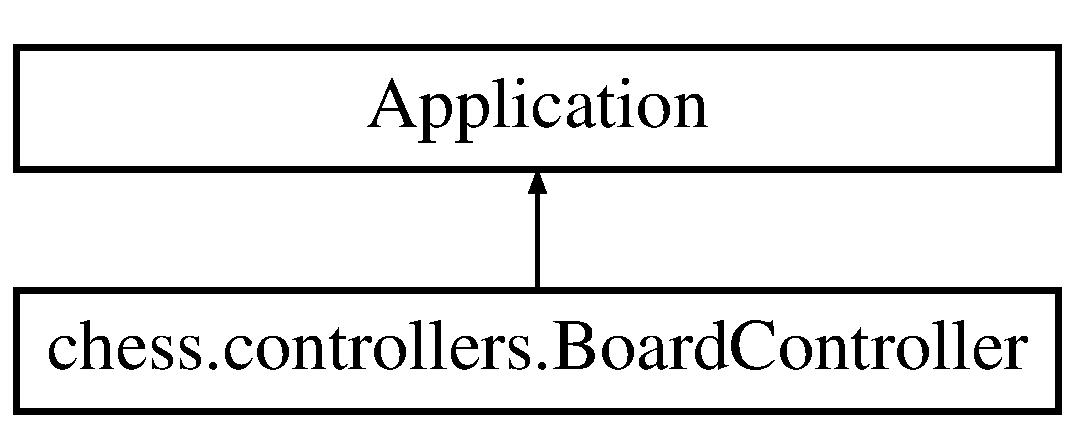
\includegraphics[height=2.000000cm]{classchess_1_1controllers_1_1_board_controller}
\end{center}
\end{figure}
\subsection*{Public Member Functions}
\begin{DoxyCompactItemize}
\item 
void \mbox{\hyperlink{classchess_1_1controllers_1_1_board_controller_abd589cb5a8d0808c83932ffba970c747}{start}} (Stage primary\+Stage)  throws Exception 
\end{DoxyCompactItemize}
\subsection*{Static Public Member Functions}
\begin{DoxyCompactItemize}
\item 
static void \mbox{\hyperlink{classchess_1_1controllers_1_1_board_controller_a0a3fb5fc97d4e1536bd0111b96f835a6}{main}} (String\mbox{[}$\,$\mbox{]} args)
\end{DoxyCompactItemize}


\subsection{Member Function Documentation}
\mbox{\Hypertarget{classchess_1_1controllers_1_1_board_controller_a0a3fb5fc97d4e1536bd0111b96f835a6}\label{classchess_1_1controllers_1_1_board_controller_a0a3fb5fc97d4e1536bd0111b96f835a6}} 
\index{chess\+::controllers\+::\+Board\+Controller@{chess\+::controllers\+::\+Board\+Controller}!main@{main}}
\index{main@{main}!chess\+::controllers\+::\+Board\+Controller@{chess\+::controllers\+::\+Board\+Controller}}
\subsubsection{\texorpdfstring{main()}{main()}}
{\footnotesize\ttfamily static void chess.\+controllers.\+Board\+Controller.\+main (\begin{DoxyParamCaption}\item[{String \mbox{[}$\,$\mbox{]}}]{args }\end{DoxyParamCaption})\hspace{0.3cm}{\ttfamily [static]}}

\mbox{\Hypertarget{classchess_1_1controllers_1_1_board_controller_abd589cb5a8d0808c83932ffba970c747}\label{classchess_1_1controllers_1_1_board_controller_abd589cb5a8d0808c83932ffba970c747}} 
\index{chess\+::controllers\+::\+Board\+Controller@{chess\+::controllers\+::\+Board\+Controller}!start@{start}}
\index{start@{start}!chess\+::controllers\+::\+Board\+Controller@{chess\+::controllers\+::\+Board\+Controller}}
\subsubsection{\texorpdfstring{start()}{start()}}
{\footnotesize\ttfamily void chess.\+controllers.\+Board\+Controller.\+start (\begin{DoxyParamCaption}\item[{Stage}]{primary\+Stage }\end{DoxyParamCaption}) throws Exception}



The documentation for this class was generated from the following file\+:\begin{DoxyCompactItemize}
\item 
G\+:/\+Chess/src/main/java/chess/controllers/\mbox{\hyperlink{_board_controller_8java}{Board\+Controller.\+java}}\end{DoxyCompactItemize}

\hypertarget{classchess_1_1_board_test}{}\section{chess.\+Board\+Test Class Reference}
\label{classchess_1_1_board_test}\index{chess.\+Board\+Test@{chess.\+Board\+Test}}
\subsection*{Public Member Functions}
\begin{DoxyCompactItemize}
\item 
void \mbox{\hyperlink{classchess_1_1_board_test_acd0ea30fd3e9742c6b71a5ee60b65707}{set\+Up}} ()
\item 
void \mbox{\hyperlink{classchess_1_1_board_test_a74abc15f67e30a9464758c1bf5dccbff}{init}} ()
\item 
void \mbox{\hyperlink{classchess_1_1_board_test_abd189ec57b7236f5482df6d2121898e6}{is\+Legal\+Move}} ()
\item 
void \mbox{\hyperlink{classchess_1_1_board_test_a844fc9d2b643df169a9b74a1983ce9ba}{is\+Over\+Piece}} ()
\item 
void \mbox{\hyperlink{classchess_1_1_board_test_ad2614964ffa53b71ba2cccc28e103132}{chess\+Move}} ()
\item 
void \mbox{\hyperlink{classchess_1_1_board_test_a61544e4031a24421423696beafba0022}{judge1}} ()
\item 
void \mbox{\hyperlink{classchess_1_1_board_test_a121d3fd4216f8b9cc947dff29a6f8dc9}{judge2}} ()
\item 
void \mbox{\hyperlink{classchess_1_1_board_test_a34e4acc21cdd11b3030d00a6d183c210}{judge3}} ()
\item 
void \mbox{\hyperlink{classchess_1_1_board_test_ac6238a4f2c53d80beb75fd43eb0aa754}{judge4}} ()
\end{DoxyCompactItemize}
\subsection*{Private Attributes}
\begin{DoxyCompactItemize}
\item 
\mbox{\hyperlink{classchess_1_1models_1_1_board}{Board}} \mbox{\hyperlink{classchess_1_1_board_test_a678a57765fd143e9c65eb0c6f741221c}{board}}
\end{DoxyCompactItemize}


\subsection{Member Function Documentation}
\mbox{\Hypertarget{classchess_1_1_board_test_ad2614964ffa53b71ba2cccc28e103132}\label{classchess_1_1_board_test_ad2614964ffa53b71ba2cccc28e103132}} 
\index{chess\+::\+Board\+Test@{chess\+::\+Board\+Test}!chess\+Move@{chess\+Move}}
\index{chess\+Move@{chess\+Move}!chess\+::\+Board\+Test@{chess\+::\+Board\+Test}}
\subsubsection{\texorpdfstring{chess\+Move()}{chessMove()}}
{\footnotesize\ttfamily void chess.\+Board\+Test.\+chess\+Move (\begin{DoxyParamCaption}{ }\end{DoxyParamCaption})}

\mbox{\Hypertarget{classchess_1_1_board_test_a74abc15f67e30a9464758c1bf5dccbff}\label{classchess_1_1_board_test_a74abc15f67e30a9464758c1bf5dccbff}} 
\index{chess\+::\+Board\+Test@{chess\+::\+Board\+Test}!init@{init}}
\index{init@{init}!chess\+::\+Board\+Test@{chess\+::\+Board\+Test}}
\subsubsection{\texorpdfstring{init()}{init()}}
{\footnotesize\ttfamily void chess.\+Board\+Test.\+init (\begin{DoxyParamCaption}{ }\end{DoxyParamCaption})}

\mbox{\Hypertarget{classchess_1_1_board_test_abd189ec57b7236f5482df6d2121898e6}\label{classchess_1_1_board_test_abd189ec57b7236f5482df6d2121898e6}} 
\index{chess\+::\+Board\+Test@{chess\+::\+Board\+Test}!is\+Legal\+Move@{is\+Legal\+Move}}
\index{is\+Legal\+Move@{is\+Legal\+Move}!chess\+::\+Board\+Test@{chess\+::\+Board\+Test}}
\subsubsection{\texorpdfstring{is\+Legal\+Move()}{isLegalMove()}}
{\footnotesize\ttfamily void chess.\+Board\+Test.\+is\+Legal\+Move (\begin{DoxyParamCaption}{ }\end{DoxyParamCaption})}

\mbox{\Hypertarget{classchess_1_1_board_test_a844fc9d2b643df169a9b74a1983ce9ba}\label{classchess_1_1_board_test_a844fc9d2b643df169a9b74a1983ce9ba}} 
\index{chess\+::\+Board\+Test@{chess\+::\+Board\+Test}!is\+Over\+Piece@{is\+Over\+Piece}}
\index{is\+Over\+Piece@{is\+Over\+Piece}!chess\+::\+Board\+Test@{chess\+::\+Board\+Test}}
\subsubsection{\texorpdfstring{is\+Over\+Piece()}{isOverPiece()}}
{\footnotesize\ttfamily void chess.\+Board\+Test.\+is\+Over\+Piece (\begin{DoxyParamCaption}{ }\end{DoxyParamCaption})}

\mbox{\Hypertarget{classchess_1_1_board_test_a61544e4031a24421423696beafba0022}\label{classchess_1_1_board_test_a61544e4031a24421423696beafba0022}} 
\index{chess\+::\+Board\+Test@{chess\+::\+Board\+Test}!judge1@{judge1}}
\index{judge1@{judge1}!chess\+::\+Board\+Test@{chess\+::\+Board\+Test}}
\subsubsection{\texorpdfstring{judge1()}{judge1()}}
{\footnotesize\ttfamily void chess.\+Board\+Test.\+judge1 (\begin{DoxyParamCaption}{ }\end{DoxyParamCaption})}

\mbox{\Hypertarget{classchess_1_1_board_test_a121d3fd4216f8b9cc947dff29a6f8dc9}\label{classchess_1_1_board_test_a121d3fd4216f8b9cc947dff29a6f8dc9}} 
\index{chess\+::\+Board\+Test@{chess\+::\+Board\+Test}!judge2@{judge2}}
\index{judge2@{judge2}!chess\+::\+Board\+Test@{chess\+::\+Board\+Test}}
\subsubsection{\texorpdfstring{judge2()}{judge2()}}
{\footnotesize\ttfamily void chess.\+Board\+Test.\+judge2 (\begin{DoxyParamCaption}{ }\end{DoxyParamCaption})}

\mbox{\Hypertarget{classchess_1_1_board_test_a34e4acc21cdd11b3030d00a6d183c210}\label{classchess_1_1_board_test_a34e4acc21cdd11b3030d00a6d183c210}} 
\index{chess\+::\+Board\+Test@{chess\+::\+Board\+Test}!judge3@{judge3}}
\index{judge3@{judge3}!chess\+::\+Board\+Test@{chess\+::\+Board\+Test}}
\subsubsection{\texorpdfstring{judge3()}{judge3()}}
{\footnotesize\ttfamily void chess.\+Board\+Test.\+judge3 (\begin{DoxyParamCaption}{ }\end{DoxyParamCaption})}

\mbox{\Hypertarget{classchess_1_1_board_test_ac6238a4f2c53d80beb75fd43eb0aa754}\label{classchess_1_1_board_test_ac6238a4f2c53d80beb75fd43eb0aa754}} 
\index{chess\+::\+Board\+Test@{chess\+::\+Board\+Test}!judge4@{judge4}}
\index{judge4@{judge4}!chess\+::\+Board\+Test@{chess\+::\+Board\+Test}}
\subsubsection{\texorpdfstring{judge4()}{judge4()}}
{\footnotesize\ttfamily void chess.\+Board\+Test.\+judge4 (\begin{DoxyParamCaption}{ }\end{DoxyParamCaption})}

\mbox{\Hypertarget{classchess_1_1_board_test_acd0ea30fd3e9742c6b71a5ee60b65707}\label{classchess_1_1_board_test_acd0ea30fd3e9742c6b71a5ee60b65707}} 
\index{chess\+::\+Board\+Test@{chess\+::\+Board\+Test}!set\+Up@{set\+Up}}
\index{set\+Up@{set\+Up}!chess\+::\+Board\+Test@{chess\+::\+Board\+Test}}
\subsubsection{\texorpdfstring{set\+Up()}{setUp()}}
{\footnotesize\ttfamily void chess.\+Board\+Test.\+set\+Up (\begin{DoxyParamCaption}{ }\end{DoxyParamCaption})}



\subsection{Member Data Documentation}
\mbox{\Hypertarget{classchess_1_1_board_test_a678a57765fd143e9c65eb0c6f741221c}\label{classchess_1_1_board_test_a678a57765fd143e9c65eb0c6f741221c}} 
\index{chess\+::\+Board\+Test@{chess\+::\+Board\+Test}!board@{board}}
\index{board@{board}!chess\+::\+Board\+Test@{chess\+::\+Board\+Test}}
\subsubsection{\texorpdfstring{board}{board}}
{\footnotesize\ttfamily \mbox{\hyperlink{classchess_1_1models_1_1_board}{Board}} chess.\+Board\+Test.\+board\hspace{0.3cm}{\ttfamily [private]}}



The documentation for this class was generated from the following file\+:\begin{DoxyCompactItemize}
\item 
G\+:/\+Chess/src/test/java/chess/\mbox{\hyperlink{_board_test_8java}{Board\+Test.\+java}}\end{DoxyCompactItemize}

\hypertarget{classchess_1_1command_1_1_chess_move}{}\section{chess.\+command.\+Chess\+Move Class Reference}
\label{classchess_1_1command_1_1_chess_move}\index{chess.\+command.\+Chess\+Move@{chess.\+command.\+Chess\+Move}}
\subsection*{Public Member Functions}
\begin{DoxyCompactItemize}
\item 
\mbox{\hyperlink{enumchess_1_1models_1_1enums_1_1_move_result}{Move\+Result}} \mbox{\hyperlink{classchess_1_1command_1_1_chess_move_a9d123dab6ec00e09fd72790dae809197}{move}} (\mbox{\hyperlink{classchess_1_1models_1_1_board}{Board}} board, \mbox{\hyperlink{classchess_1_1models_1_1_chess_piece}{Chess\+Piece}} chess, \mbox{\hyperlink{classchess_1_1models_1_1_position}{Position}} destination)
\end{DoxyCompactItemize}


\subsection{Detailed Description}
Receiver of the \mbox{\hyperlink{interfacechess_1_1command_1_1_command}{Command}} Pattern 

\subsection{Member Function Documentation}
\mbox{\Hypertarget{classchess_1_1command_1_1_chess_move_a9d123dab6ec00e09fd72790dae809197}\label{classchess_1_1command_1_1_chess_move_a9d123dab6ec00e09fd72790dae809197}} 
\index{chess\+::command\+::\+Chess\+Move@{chess\+::command\+::\+Chess\+Move}!move@{move}}
\index{move@{move}!chess\+::command\+::\+Chess\+Move@{chess\+::command\+::\+Chess\+Move}}
\subsubsection{\texorpdfstring{move()}{move()}}
{\footnotesize\ttfamily \mbox{\hyperlink{enumchess_1_1models_1_1enums_1_1_move_result}{Move\+Result}} chess.\+command.\+Chess\+Move.\+move (\begin{DoxyParamCaption}\item[{\mbox{\hyperlink{classchess_1_1models_1_1_board}{Board}}}]{board,  }\item[{\mbox{\hyperlink{classchess_1_1models_1_1_chess_piece}{Chess\+Piece}}}]{chess,  }\item[{\mbox{\hyperlink{classchess_1_1models_1_1_position}{Position}}}]{destination }\end{DoxyParamCaption})}

Move a piece to specific position on the board


\begin{DoxyParams}{Parameters}
{\em board} & Chess board \\
\hline
{\em chess} & Piece that needs to move \\
\hline
{\em destination} & Destination position \\
\hline
\end{DoxyParams}


The documentation for this class was generated from the following file\+:\begin{DoxyCompactItemize}
\item 
src/main/java/chess/command/\mbox{\hyperlink{_chess_move_8java}{Chess\+Move.\+java}}\end{DoxyCompactItemize}

\hypertarget{classchess_1_1command_1_1_chess_move_command}{}\section{chess.\+command.\+Chess\+Move\+Command Class Reference}
\label{classchess_1_1command_1_1_chess_move_command}\index{chess.\+command.\+Chess\+Move\+Command@{chess.\+command.\+Chess\+Move\+Command}}
Inheritance diagram for chess.\+command.\+Chess\+Move\+Command\+:\begin{figure}[H]
\begin{center}
\leavevmode
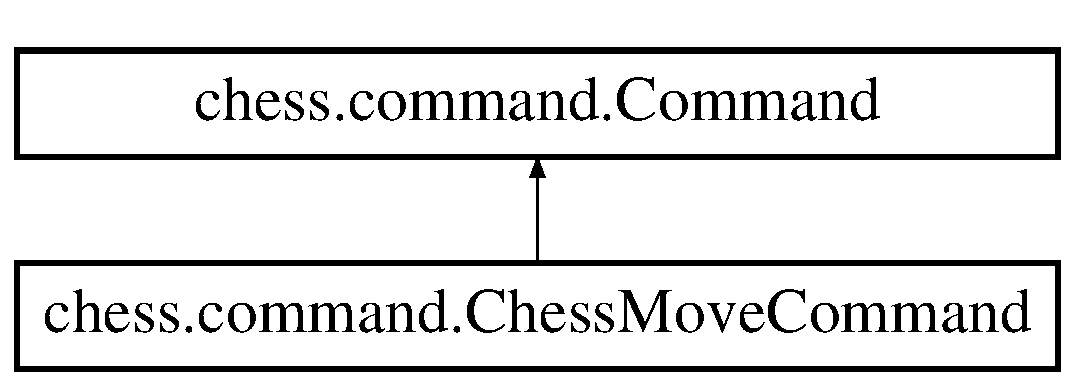
\includegraphics[height=2.000000cm]{classchess_1_1command_1_1_chess_move_command}
\end{center}
\end{figure}
\subsection*{Public Member Functions}
\begin{DoxyCompactItemize}
\item 
\mbox{\hyperlink{classchess_1_1command_1_1_chess_move_command_a015eb289219c05fd0ee4009d939b25bc}{Chess\+Move\+Command}} (\mbox{\hyperlink{classchess_1_1command_1_1_chess_move}{Chess\+Move}} chess\+Move)
\item 
\mbox{\hyperlink{enumchess_1_1models_1_1enums_1_1_move_result}{Move\+Result}} \mbox{\hyperlink{classchess_1_1command_1_1_chess_move_command_a7a74fa700b53038f06de08a11699d37e}{execute}} (\mbox{\hyperlink{classchess_1_1models_1_1_board}{Board}} board, \mbox{\hyperlink{classchess_1_1models_1_1_chess_piece}{Chess\+Piece}} chess, \mbox{\hyperlink{classchess_1_1models_1_1_position}{Position}} destination)
\item 
List$<$ \mbox{\hyperlink{classchess_1_1models_1_1_position}{Position}} $>$ \mbox{\hyperlink{classchess_1_1command_1_1_chess_move_command_a31a0cc0d4b19d5441f9420e0d4c1a795}{undo}} (\mbox{\hyperlink{classchess_1_1models_1_1_board}{Board}} board)
\end{DoxyCompactItemize}


\subsection{Detailed Description}
Implement of the command interface 

\subsection{Constructor \& Destructor Documentation}
\mbox{\Hypertarget{classchess_1_1command_1_1_chess_move_command_a015eb289219c05fd0ee4009d939b25bc}\label{classchess_1_1command_1_1_chess_move_command_a015eb289219c05fd0ee4009d939b25bc}} 
\index{chess\+::command\+::\+Chess\+Move\+Command@{chess\+::command\+::\+Chess\+Move\+Command}!Chess\+Move\+Command@{Chess\+Move\+Command}}
\index{Chess\+Move\+Command@{Chess\+Move\+Command}!chess\+::command\+::\+Chess\+Move\+Command@{chess\+::command\+::\+Chess\+Move\+Command}}
\subsubsection{\texorpdfstring{Chess\+Move\+Command()}{ChessMoveCommand()}}
{\footnotesize\ttfamily chess.\+command.\+Chess\+Move\+Command.\+Chess\+Move\+Command (\begin{DoxyParamCaption}\item[{\mbox{\hyperlink{classchess_1_1command_1_1_chess_move}{Chess\+Move}}}]{chess\+Move }\end{DoxyParamCaption})}

Contructor of \mbox{\hyperlink{classchess_1_1command_1_1_chess_move_command}{Chess\+Move\+Command}}


\begin{DoxyParams}{Parameters}
{\em chess\+Move} & Receiver of the \mbox{\hyperlink{interfacechess_1_1command_1_1_command}{Command}} Pattern \\
\hline
\end{DoxyParams}


\subsection{Member Function Documentation}
\mbox{\Hypertarget{classchess_1_1command_1_1_chess_move_command_a7a74fa700b53038f06de08a11699d37e}\label{classchess_1_1command_1_1_chess_move_command_a7a74fa700b53038f06de08a11699d37e}} 
\index{chess\+::command\+::\+Chess\+Move\+Command@{chess\+::command\+::\+Chess\+Move\+Command}!execute@{execute}}
\index{execute@{execute}!chess\+::command\+::\+Chess\+Move\+Command@{chess\+::command\+::\+Chess\+Move\+Command}}
\subsubsection{\texorpdfstring{execute()}{execute()}}
{\footnotesize\ttfamily \mbox{\hyperlink{enumchess_1_1models_1_1enums_1_1_move_result}{Move\+Result}} chess.\+command.\+Chess\+Move\+Command.\+execute (\begin{DoxyParamCaption}\item[{\mbox{\hyperlink{classchess_1_1models_1_1_board}{Board}}}]{board,  }\item[{\mbox{\hyperlink{classchess_1_1models_1_1_chess_piece}{Chess\+Piece}}}]{chess,  }\item[{\mbox{\hyperlink{classchess_1_1models_1_1_position}{Position}}}]{destination }\end{DoxyParamCaption})}

Execute command


\begin{DoxyParams}{Parameters}
{\em board} & Chess board \\
\hline
{\em chess} & Piece that needs to move \\
\hline
{\em destination} & Destination position \\
\hline
\end{DoxyParams}


Implements \mbox{\hyperlink{interfacechess_1_1command_1_1_command_a93071fc9ddc45d04e7c8e42cc78b5d6c}{chess.\+command.\+Command}}.

\mbox{\Hypertarget{classchess_1_1command_1_1_chess_move_command_a31a0cc0d4b19d5441f9420e0d4c1a795}\label{classchess_1_1command_1_1_chess_move_command_a31a0cc0d4b19d5441f9420e0d4c1a795}} 
\index{chess\+::command\+::\+Chess\+Move\+Command@{chess\+::command\+::\+Chess\+Move\+Command}!undo@{undo}}
\index{undo@{undo}!chess\+::command\+::\+Chess\+Move\+Command@{chess\+::command\+::\+Chess\+Move\+Command}}
\subsubsection{\texorpdfstring{undo()}{undo()}}
{\footnotesize\ttfamily List$<$\mbox{\hyperlink{classchess_1_1models_1_1_position}{Position}}$>$ chess.\+command.\+Chess\+Move\+Command.\+undo (\begin{DoxyParamCaption}\item[{\mbox{\hyperlink{classchess_1_1models_1_1_board}{Board}}}]{board }\end{DoxyParamCaption})}

Undo command


\begin{DoxyParams}{Parameters}
{\em board} & Chess board \\
\hline
\end{DoxyParams}
\begin{DoxyReturn}{Returns}
The chess\textquotesingle{}s positions before undo and after undo 
\end{DoxyReturn}


Implements \mbox{\hyperlink{interfacechess_1_1command_1_1_command_a7e407e4a40124384e8262aa573fbeaac}{chess.\+command.\+Command}}.



The documentation for this class was generated from the following file\+:\begin{DoxyCompactItemize}
\item 
src/main/java/chess/command/\mbox{\hyperlink{_chess_move_command_8java}{Chess\+Move\+Command.\+java}}\end{DoxyCompactItemize}

\hypertarget{classchess_1_1models_1_1_chess_piece}{}\section{chess.\+models.\+Chess\+Piece Class Reference}
\label{classchess_1_1models_1_1_chess_piece}\index{chess.\+models.\+Chess\+Piece@{chess.\+models.\+Chess\+Piece}}
Inheritance diagram for chess.\+models.\+Chess\+Piece\+:\begin{figure}[H]
\begin{center}
\leavevmode
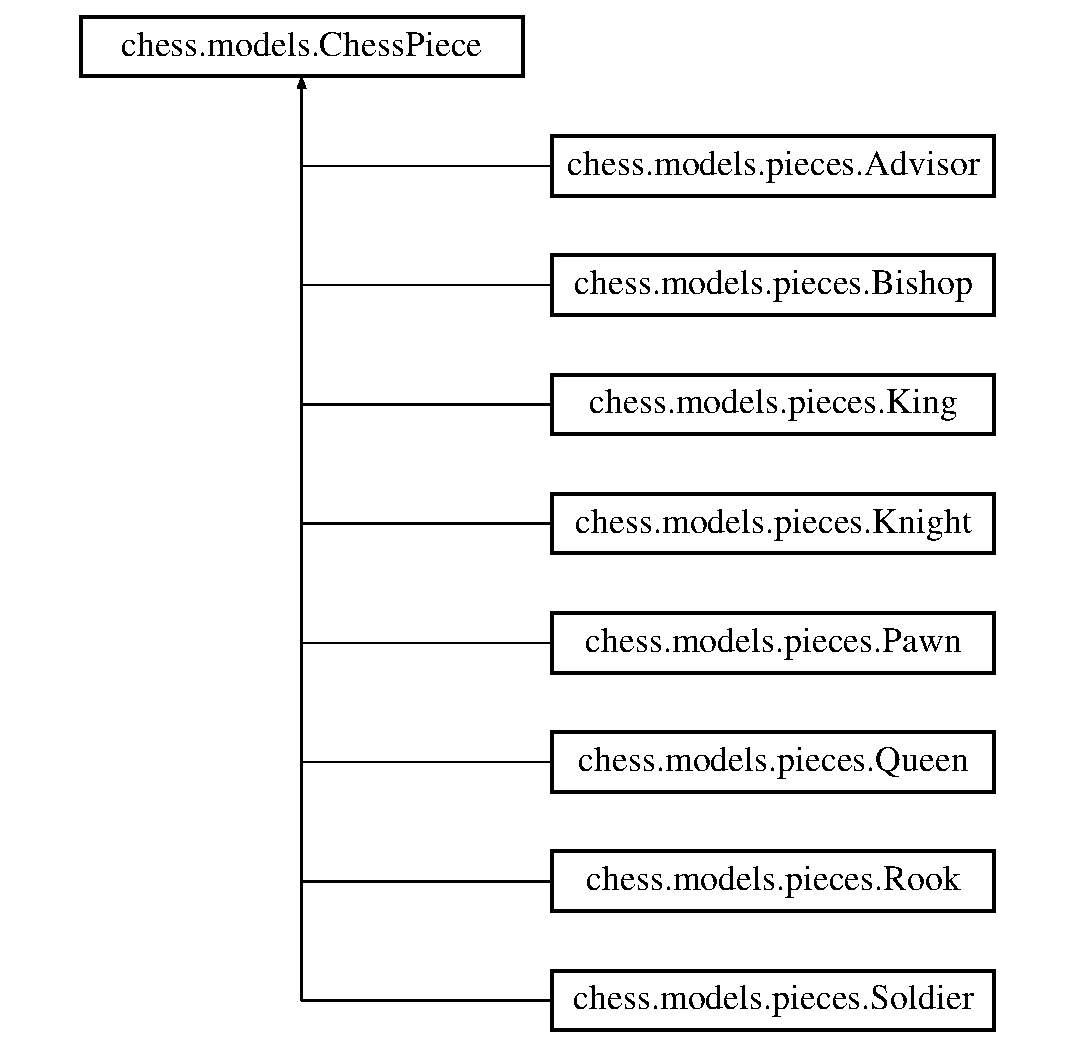
\includegraphics[height=9.000000cm]{classchess_1_1models_1_1_chess_piece}
\end{center}
\end{figure}
\subsection*{Public Member Functions}
\begin{DoxyCompactItemize}
\item 
\mbox{\hyperlink{classchess_1_1models_1_1_chess_piece_a59beae5e1f384747a201a4c417ca0afb}{Chess\+Piece}} (\mbox{\hyperlink{enumchess_1_1models_1_1enums_1_1_player}{Player}} player, \mbox{\hyperlink{classchess_1_1models_1_1_position}{Position}} position)
\item 
\mbox{\hyperlink{classchess_1_1models_1_1_chess_piece_aeea9d0c376842325301238b95cabe85c}{Chess\+Piece}} (\mbox{\hyperlink{enumchess_1_1models_1_1enums_1_1_player}{Player}} player, \mbox{\hyperlink{classchess_1_1models_1_1_position}{Position}} position, int id)
\item 
\mbox{\hyperlink{classchess_1_1models_1_1_position}{Position}} \mbox{\hyperlink{classchess_1_1models_1_1_chess_piece_a4ce783eeb2ec6d5cd83af05c11fe8cdb}{get\+Position}} ()
\item 
void \mbox{\hyperlink{classchess_1_1models_1_1_chess_piece_a2e3c62bde5041ca0aa53e0476cc8b600}{set\+Position}} (\mbox{\hyperlink{classchess_1_1models_1_1_position}{Position}} position)
\item 
\mbox{\hyperlink{enumchess_1_1models_1_1enums_1_1_player}{Player}} \mbox{\hyperlink{classchess_1_1models_1_1_chess_piece_aaa3cef5d52e4a228dc01f91133a6c437}{get\+Player}} ()
\item 
int \mbox{\hyperlink{classchess_1_1models_1_1_chess_piece_aaa0ccd6a8327325fa05f7654669516ae}{get\+Id}} ()
\item 
void \mbox{\hyperlink{classchess_1_1models_1_1_chess_piece_a77865fbd52257338c4e376af525155c7}{move}} (\mbox{\hyperlink{classchess_1_1models_1_1_position}{Position}} position)
\item 
abstract \mbox{\hyperlink{enumchess_1_1models_1_1enums_1_1_move_result}{Move\+Result}} \mbox{\hyperlink{classchess_1_1models_1_1_chess_piece_a60088166dd440bf51de4514c3e57841e}{is\+Legal\+Move}} (\mbox{\hyperlink{classchess_1_1models_1_1_position}{Position}} pos)
\item 
Set$<$ \mbox{\hyperlink{classchess_1_1models_1_1_position}{Position}} $>$ \mbox{\hyperlink{classchess_1_1models_1_1_chess_piece_afd359313e83bdef860f9f8236435522f}{gen\+Next\+Step}} (\mbox{\hyperlink{classchess_1_1models_1_1_board}{Board}} board)
\end{DoxyCompactItemize}


\subsection{Detailed Description}
All kinds of chess pieces 

\subsection{Constructor \& Destructor Documentation}
\mbox{\Hypertarget{classchess_1_1models_1_1_chess_piece_a59beae5e1f384747a201a4c417ca0afb}\label{classchess_1_1models_1_1_chess_piece_a59beae5e1f384747a201a4c417ca0afb}} 
\index{chess\+::models\+::\+Chess\+Piece@{chess\+::models\+::\+Chess\+Piece}!Chess\+Piece@{Chess\+Piece}}
\index{Chess\+Piece@{Chess\+Piece}!chess\+::models\+::\+Chess\+Piece@{chess\+::models\+::\+Chess\+Piece}}
\subsubsection{\texorpdfstring{Chess\+Piece()}{ChessPiece()}\hspace{0.1cm}{\footnotesize\ttfamily [1/2]}}
{\footnotesize\ttfamily chess.\+models.\+Chess\+Piece.\+Chess\+Piece (\begin{DoxyParamCaption}\item[{\mbox{\hyperlink{enumchess_1_1models_1_1enums_1_1_player}{Player}}}]{player,  }\item[{\mbox{\hyperlink{classchess_1_1models_1_1_position}{Position}}}]{position }\end{DoxyParamCaption})}

Constructor of \mbox{\hyperlink{classchess_1_1models_1_1_chess_piece}{Chess\+Piece}}


\begin{DoxyParams}{Parameters}
{\em player} & Belongs to which player \\
\hline
{\em position} & Initial position \\
\hline
\end{DoxyParams}
\mbox{\Hypertarget{classchess_1_1models_1_1_chess_piece_aeea9d0c376842325301238b95cabe85c}\label{classchess_1_1models_1_1_chess_piece_aeea9d0c376842325301238b95cabe85c}} 
\index{chess\+::models\+::\+Chess\+Piece@{chess\+::models\+::\+Chess\+Piece}!Chess\+Piece@{Chess\+Piece}}
\index{Chess\+Piece@{Chess\+Piece}!chess\+::models\+::\+Chess\+Piece@{chess\+::models\+::\+Chess\+Piece}}
\subsubsection{\texorpdfstring{Chess\+Piece()}{ChessPiece()}\hspace{0.1cm}{\footnotesize\ttfamily [2/2]}}
{\footnotesize\ttfamily chess.\+models.\+Chess\+Piece.\+Chess\+Piece (\begin{DoxyParamCaption}\item[{\mbox{\hyperlink{enumchess_1_1models_1_1enums_1_1_player}{Player}}}]{player,  }\item[{\mbox{\hyperlink{classchess_1_1models_1_1_position}{Position}}}]{position,  }\item[{int}]{id }\end{DoxyParamCaption})}



\subsection{Member Function Documentation}
\mbox{\Hypertarget{classchess_1_1models_1_1_chess_piece_afd359313e83bdef860f9f8236435522f}\label{classchess_1_1models_1_1_chess_piece_afd359313e83bdef860f9f8236435522f}} 
\index{chess\+::models\+::\+Chess\+Piece@{chess\+::models\+::\+Chess\+Piece}!gen\+Next\+Step@{gen\+Next\+Step}}
\index{gen\+Next\+Step@{gen\+Next\+Step}!chess\+::models\+::\+Chess\+Piece@{chess\+::models\+::\+Chess\+Piece}}
\subsubsection{\texorpdfstring{gen\+Next\+Step()}{genNextStep()}}
{\footnotesize\ttfamily Set$<$\mbox{\hyperlink{classchess_1_1models_1_1_position}{Position}}$>$ chess.\+models.\+Chess\+Piece.\+gen\+Next\+Step (\begin{DoxyParamCaption}\item[{\mbox{\hyperlink{classchess_1_1models_1_1_board}{Board}}}]{board }\end{DoxyParamCaption})}

Generate all possible next steps of the chess


\begin{DoxyParams}{Parameters}
{\em board} & the chess board \\
\hline
\end{DoxyParams}
\begin{DoxyReturn}{Returns}
all possible next steps of the chess 
\end{DoxyReturn}
\mbox{\Hypertarget{classchess_1_1models_1_1_chess_piece_aaa0ccd6a8327325fa05f7654669516ae}\label{classchess_1_1models_1_1_chess_piece_aaa0ccd6a8327325fa05f7654669516ae}} 
\index{chess\+::models\+::\+Chess\+Piece@{chess\+::models\+::\+Chess\+Piece}!get\+Id@{get\+Id}}
\index{get\+Id@{get\+Id}!chess\+::models\+::\+Chess\+Piece@{chess\+::models\+::\+Chess\+Piece}}
\subsubsection{\texorpdfstring{get\+Id()}{getId()}}
{\footnotesize\ttfamily int chess.\+models.\+Chess\+Piece.\+get\+Id (\begin{DoxyParamCaption}{ }\end{DoxyParamCaption})}

Get the piece\textquotesingle{}s id

\begin{DoxyReturn}{Returns}
the piece\textquotesingle{}s id 
\end{DoxyReturn}
\mbox{\Hypertarget{classchess_1_1models_1_1_chess_piece_aaa3cef5d52e4a228dc01f91133a6c437}\label{classchess_1_1models_1_1_chess_piece_aaa3cef5d52e4a228dc01f91133a6c437}} 
\index{chess\+::models\+::\+Chess\+Piece@{chess\+::models\+::\+Chess\+Piece}!get\+Player@{get\+Player}}
\index{get\+Player@{get\+Player}!chess\+::models\+::\+Chess\+Piece@{chess\+::models\+::\+Chess\+Piece}}
\subsubsection{\texorpdfstring{get\+Player()}{getPlayer()}}
{\footnotesize\ttfamily \mbox{\hyperlink{enumchess_1_1models_1_1enums_1_1_player}{Player}} chess.\+models.\+Chess\+Piece.\+get\+Player (\begin{DoxyParamCaption}{ }\end{DoxyParamCaption})}

Get player this piece belongs to

\begin{DoxyReturn}{Returns}
player this piece belongs to 
\end{DoxyReturn}
\mbox{\Hypertarget{classchess_1_1models_1_1_chess_piece_a4ce783eeb2ec6d5cd83af05c11fe8cdb}\label{classchess_1_1models_1_1_chess_piece_a4ce783eeb2ec6d5cd83af05c11fe8cdb}} 
\index{chess\+::models\+::\+Chess\+Piece@{chess\+::models\+::\+Chess\+Piece}!get\+Position@{get\+Position}}
\index{get\+Position@{get\+Position}!chess\+::models\+::\+Chess\+Piece@{chess\+::models\+::\+Chess\+Piece}}
\subsubsection{\texorpdfstring{get\+Position()}{getPosition()}}
{\footnotesize\ttfamily \mbox{\hyperlink{classchess_1_1models_1_1_position}{Position}} chess.\+models.\+Chess\+Piece.\+get\+Position (\begin{DoxyParamCaption}{ }\end{DoxyParamCaption})}

Get current position

\begin{DoxyReturn}{Returns}
current position 
\end{DoxyReturn}
\mbox{\Hypertarget{classchess_1_1models_1_1_chess_piece_a60088166dd440bf51de4514c3e57841e}\label{classchess_1_1models_1_1_chess_piece_a60088166dd440bf51de4514c3e57841e}} 
\index{chess\+::models\+::\+Chess\+Piece@{chess\+::models\+::\+Chess\+Piece}!is\+Legal\+Move@{is\+Legal\+Move}}
\index{is\+Legal\+Move@{is\+Legal\+Move}!chess\+::models\+::\+Chess\+Piece@{chess\+::models\+::\+Chess\+Piece}}
\subsubsection{\texorpdfstring{is\+Legal\+Move()}{isLegalMove()}}
{\footnotesize\ttfamily abstract \mbox{\hyperlink{enumchess_1_1models_1_1enums_1_1_move_result}{Move\+Result}} chess.\+models.\+Chess\+Piece.\+is\+Legal\+Move (\begin{DoxyParamCaption}\item[{\mbox{\hyperlink{classchess_1_1models_1_1_position}{Position}}}]{pos }\end{DoxyParamCaption})\hspace{0.3cm}{\ttfamily [abstract]}}

Check if the movement is legal


\begin{DoxyParams}{Parameters}
{\em pos} & destination position \\
\hline
\end{DoxyParams}
\begin{DoxyReturn}{Returns}
Move\+Result 
\end{DoxyReturn}
\mbox{\Hypertarget{classchess_1_1models_1_1_chess_piece_a77865fbd52257338c4e376af525155c7}\label{classchess_1_1models_1_1_chess_piece_a77865fbd52257338c4e376af525155c7}} 
\index{chess\+::models\+::\+Chess\+Piece@{chess\+::models\+::\+Chess\+Piece}!move@{move}}
\index{move@{move}!chess\+::models\+::\+Chess\+Piece@{chess\+::models\+::\+Chess\+Piece}}
\subsubsection{\texorpdfstring{move()}{move()}}
{\footnotesize\ttfamily void chess.\+models.\+Chess\+Piece.\+move (\begin{DoxyParamCaption}\item[{\mbox{\hyperlink{classchess_1_1models_1_1_position}{Position}}}]{position }\end{DoxyParamCaption})}

Move to specific position


\begin{DoxyParams}{Parameters}
{\em position} & specific position \\
\hline
\end{DoxyParams}
\mbox{\Hypertarget{classchess_1_1models_1_1_chess_piece_a2e3c62bde5041ca0aa53e0476cc8b600}\label{classchess_1_1models_1_1_chess_piece_a2e3c62bde5041ca0aa53e0476cc8b600}} 
\index{chess\+::models\+::\+Chess\+Piece@{chess\+::models\+::\+Chess\+Piece}!set\+Position@{set\+Position}}
\index{set\+Position@{set\+Position}!chess\+::models\+::\+Chess\+Piece@{chess\+::models\+::\+Chess\+Piece}}
\subsubsection{\texorpdfstring{set\+Position()}{setPosition()}}
{\footnotesize\ttfamily void chess.\+models.\+Chess\+Piece.\+set\+Position (\begin{DoxyParamCaption}\item[{\mbox{\hyperlink{classchess_1_1models_1_1_position}{Position}}}]{position }\end{DoxyParamCaption})}

Set chess piece position


\begin{DoxyParams}{Parameters}
{\em position} & specific position \\
\hline
\end{DoxyParams}


The documentation for this class was generated from the following file\+:\begin{DoxyCompactItemize}
\item 
src/main/java/chess/models/\mbox{\hyperlink{_chess_piece_8java}{Chess\+Piece.\+java}}\end{DoxyCompactItemize}

\hypertarget{interfacechess_1_1command_1_1_command}{}\section{chess.\+command.\+Command Interface Reference}
\label{interfacechess_1_1command_1_1_command}\index{chess.\+command.\+Command@{chess.\+command.\+Command}}
Inheritance diagram for chess.\+command.\+Command\+:\begin{figure}[H]
\begin{center}
\leavevmode
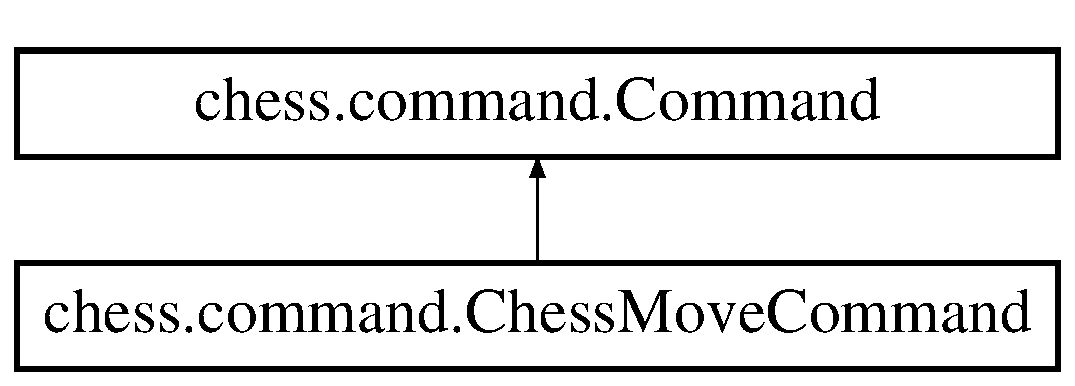
\includegraphics[height=2.000000cm]{interfacechess_1_1command_1_1_command}
\end{center}
\end{figure}
\subsection*{Public Member Functions}
\begin{DoxyCompactItemize}
\item 
\mbox{\hyperlink{enumchess_1_1models_1_1enums_1_1_move_result}{Move\+Result}} \mbox{\hyperlink{interfacechess_1_1command_1_1_command_a93071fc9ddc45d04e7c8e42cc78b5d6c}{execute}} (\mbox{\hyperlink{classchess_1_1models_1_1_board}{Board}} board, \mbox{\hyperlink{classchess_1_1models_1_1_chess_piece}{Chess\+Piece}} chess, \mbox{\hyperlink{classchess_1_1models_1_1_position}{Position}} destination)
\item 
List$<$ \mbox{\hyperlink{classchess_1_1models_1_1_position}{Position}} $>$ \mbox{\hyperlink{interfacechess_1_1command_1_1_command_a7e407e4a40124384e8262aa573fbeaac}{undo}} (\mbox{\hyperlink{classchess_1_1models_1_1_board}{Board}} board)
\end{DoxyCompactItemize}


\subsection{Detailed Description}
The command interface of the \mbox{\hyperlink{interfacechess_1_1command_1_1_command}{Command}} Pattern 

\subsection{Member Function Documentation}
\mbox{\Hypertarget{interfacechess_1_1command_1_1_command_a93071fc9ddc45d04e7c8e42cc78b5d6c}\label{interfacechess_1_1command_1_1_command_a93071fc9ddc45d04e7c8e42cc78b5d6c}} 
\index{chess\+::command\+::\+Command@{chess\+::command\+::\+Command}!execute@{execute}}
\index{execute@{execute}!chess\+::command\+::\+Command@{chess\+::command\+::\+Command}}
\subsubsection{\texorpdfstring{execute()}{execute()}}
{\footnotesize\ttfamily \mbox{\hyperlink{enumchess_1_1models_1_1enums_1_1_move_result}{Move\+Result}} chess.\+command.\+Command.\+execute (\begin{DoxyParamCaption}\item[{\mbox{\hyperlink{classchess_1_1models_1_1_board}{Board}}}]{board,  }\item[{\mbox{\hyperlink{classchess_1_1models_1_1_chess_piece}{Chess\+Piece}}}]{chess,  }\item[{\mbox{\hyperlink{classchess_1_1models_1_1_position}{Position}}}]{destination }\end{DoxyParamCaption})}



Implemented in \mbox{\hyperlink{classchess_1_1command_1_1_chess_move_command_a7a74fa700b53038f06de08a11699d37e}{chess.\+command.\+Chess\+Move\+Command}}.

\mbox{\Hypertarget{interfacechess_1_1command_1_1_command_a7e407e4a40124384e8262aa573fbeaac}\label{interfacechess_1_1command_1_1_command_a7e407e4a40124384e8262aa573fbeaac}} 
\index{chess\+::command\+::\+Command@{chess\+::command\+::\+Command}!undo@{undo}}
\index{undo@{undo}!chess\+::command\+::\+Command@{chess\+::command\+::\+Command}}
\subsubsection{\texorpdfstring{undo()}{undo()}}
{\footnotesize\ttfamily List$<$\mbox{\hyperlink{classchess_1_1models_1_1_position}{Position}}$>$ chess.\+command.\+Command.\+undo (\begin{DoxyParamCaption}\item[{\mbox{\hyperlink{classchess_1_1models_1_1_board}{Board}}}]{board }\end{DoxyParamCaption})}



Implemented in \mbox{\hyperlink{classchess_1_1command_1_1_chess_move_command_a31a0cc0d4b19d5441f9420e0d4c1a795}{chess.\+command.\+Chess\+Move\+Command}}.



The documentation for this interface was generated from the following file\+:\begin{DoxyCompactItemize}
\item 
src/main/java/chess/command/\mbox{\hyperlink{_command_8java}{Command.\+java}}\end{DoxyCompactItemize}

\hypertarget{enumchess_1_1models_1_1enums_1_1_game_mode}{}\section{chess.\+models.\+enums.\+Game\+Mode Enum Reference}
\label{enumchess_1_1models_1_1enums_1_1_game_mode}\index{chess.\+models.\+enums.\+Game\+Mode@{chess.\+models.\+enums.\+Game\+Mode}}
\subsection*{Public Attributes}
\begin{DoxyCompactItemize}
\item 
\mbox{\hyperlink{enumchess_1_1models_1_1enums_1_1_game_mode_ac77c07197becd077c3c5bb8906f60b1e}{Classic}}
\item 
\mbox{\hyperlink{enumchess_1_1models_1_1enums_1_1_game_mode_a4f5517a647fcb4190a521a8b5d7cf0b0}{New}}
\end{DoxyCompactItemize}


\subsection{Member Data Documentation}
\mbox{\Hypertarget{enumchess_1_1models_1_1enums_1_1_game_mode_ac77c07197becd077c3c5bb8906f60b1e}\label{enumchess_1_1models_1_1enums_1_1_game_mode_ac77c07197becd077c3c5bb8906f60b1e}} 
\index{chess\+::models\+::enums\+::\+Game\+Mode@{chess\+::models\+::enums\+::\+Game\+Mode}!Classic@{Classic}}
\index{Classic@{Classic}!chess\+::models\+::enums\+::\+Game\+Mode@{chess\+::models\+::enums\+::\+Game\+Mode}}
\subsubsection{\texorpdfstring{Classic}{Classic}}
{\footnotesize\ttfamily chess.\+models.\+enums.\+Game\+Mode.\+Classic}

\mbox{\Hypertarget{enumchess_1_1models_1_1enums_1_1_game_mode_a4f5517a647fcb4190a521a8b5d7cf0b0}\label{enumchess_1_1models_1_1enums_1_1_game_mode_a4f5517a647fcb4190a521a8b5d7cf0b0}} 
\index{chess\+::models\+::enums\+::\+Game\+Mode@{chess\+::models\+::enums\+::\+Game\+Mode}!New@{New}}
\index{New@{New}!chess\+::models\+::enums\+::\+Game\+Mode@{chess\+::models\+::enums\+::\+Game\+Mode}}
\subsubsection{\texorpdfstring{New}{New}}
{\footnotesize\ttfamily chess.\+models.\+enums.\+Game\+Mode.\+New}



The documentation for this enum was generated from the following file\+:\begin{DoxyCompactItemize}
\item 
src/main/java/chess/models/enums/\mbox{\hyperlink{_game_mode_8java}{Game\+Mode.\+java}}\end{DoxyCompactItemize}

\hypertarget{enumchess_1_1models_1_1enums_1_1_game_result}{}\section{chess.\+models.\+enums.\+Game\+Result Enum Reference}
\label{enumchess_1_1models_1_1enums_1_1_game_result}\index{chess.\+models.\+enums.\+Game\+Result@{chess.\+models.\+enums.\+Game\+Result}}
\subsection*{Public Attributes}
\begin{DoxyCompactItemize}
\item 
\mbox{\hyperlink{enumchess_1_1models_1_1enums_1_1_game_result_ac45a99e6bed59ba2fa6b229383229195}{Black\+Win}}
\item 
\mbox{\hyperlink{enumchess_1_1models_1_1enums_1_1_game_result_ab484738f8e1b5994fb669ee8d6d02158}{White\+Win}}
\item 
\mbox{\hyperlink{enumchess_1_1models_1_1enums_1_1_game_result_affcb10bb1b037bc3b20972e49b91a7f0}{Draw}}
\item 
\mbox{\hyperlink{enumchess_1_1models_1_1enums_1_1_game_result_a934fd181ee21601ba0e5fb875edd150b}{Gaming}}
\end{DoxyCompactItemize}


\subsection{Member Data Documentation}
\mbox{\Hypertarget{enumchess_1_1models_1_1enums_1_1_game_result_ac45a99e6bed59ba2fa6b229383229195}\label{enumchess_1_1models_1_1enums_1_1_game_result_ac45a99e6bed59ba2fa6b229383229195}} 
\index{chess\+::models\+::enums\+::\+Game\+Result@{chess\+::models\+::enums\+::\+Game\+Result}!Black\+Win@{Black\+Win}}
\index{Black\+Win@{Black\+Win}!chess\+::models\+::enums\+::\+Game\+Result@{chess\+::models\+::enums\+::\+Game\+Result}}
\subsubsection{\texorpdfstring{Black\+Win}{BlackWin}}
{\footnotesize\ttfamily chess.\+models.\+enums.\+Game\+Result.\+Black\+Win}

\mbox{\Hypertarget{enumchess_1_1models_1_1enums_1_1_game_result_affcb10bb1b037bc3b20972e49b91a7f0}\label{enumchess_1_1models_1_1enums_1_1_game_result_affcb10bb1b037bc3b20972e49b91a7f0}} 
\index{chess\+::models\+::enums\+::\+Game\+Result@{chess\+::models\+::enums\+::\+Game\+Result}!Draw@{Draw}}
\index{Draw@{Draw}!chess\+::models\+::enums\+::\+Game\+Result@{chess\+::models\+::enums\+::\+Game\+Result}}
\subsubsection{\texorpdfstring{Draw}{Draw}}
{\footnotesize\ttfamily chess.\+models.\+enums.\+Game\+Result.\+Draw}

\mbox{\Hypertarget{enumchess_1_1models_1_1enums_1_1_game_result_a934fd181ee21601ba0e5fb875edd150b}\label{enumchess_1_1models_1_1enums_1_1_game_result_a934fd181ee21601ba0e5fb875edd150b}} 
\index{chess\+::models\+::enums\+::\+Game\+Result@{chess\+::models\+::enums\+::\+Game\+Result}!Gaming@{Gaming}}
\index{Gaming@{Gaming}!chess\+::models\+::enums\+::\+Game\+Result@{chess\+::models\+::enums\+::\+Game\+Result}}
\subsubsection{\texorpdfstring{Gaming}{Gaming}}
{\footnotesize\ttfamily chess.\+models.\+enums.\+Game\+Result.\+Gaming}

\mbox{\Hypertarget{enumchess_1_1models_1_1enums_1_1_game_result_ab484738f8e1b5994fb669ee8d6d02158}\label{enumchess_1_1models_1_1enums_1_1_game_result_ab484738f8e1b5994fb669ee8d6d02158}} 
\index{chess\+::models\+::enums\+::\+Game\+Result@{chess\+::models\+::enums\+::\+Game\+Result}!White\+Win@{White\+Win}}
\index{White\+Win@{White\+Win}!chess\+::models\+::enums\+::\+Game\+Result@{chess\+::models\+::enums\+::\+Game\+Result}}
\subsubsection{\texorpdfstring{White\+Win}{WhiteWin}}
{\footnotesize\ttfamily chess.\+models.\+enums.\+Game\+Result.\+White\+Win}



The documentation for this enum was generated from the following file\+:\begin{DoxyCompactItemize}
\item 
G\+:/\+Chess/src/main/java/chess/models/enums/\mbox{\hyperlink{_game_result_8java}{Game\+Result.\+java}}\end{DoxyCompactItemize}

\hypertarget{classchess_1_1models_1_1pieces_1_1_king}{}\section{chess.\+models.\+pieces.\+King Class Reference}
\label{classchess_1_1models_1_1pieces_1_1_king}\index{chess.\+models.\+pieces.\+King@{chess.\+models.\+pieces.\+King}}
Inheritance diagram for chess.\+models.\+pieces.\+King\+:\begin{figure}[H]
\begin{center}
\leavevmode
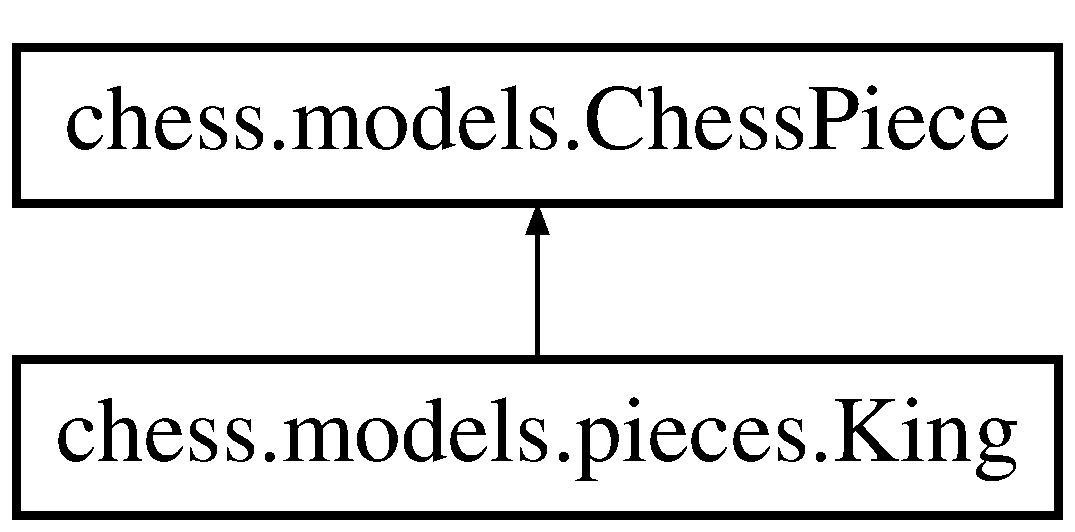
\includegraphics[height=2.000000cm]{classchess_1_1models_1_1pieces_1_1_king}
\end{center}
\end{figure}
\subsection*{Public Member Functions}
\begin{DoxyCompactItemize}
\item 
\mbox{\hyperlink{classchess_1_1models_1_1pieces_1_1_king_abc06c6362a34a9f7289c374c50d3b728}{King}} (\mbox{\hyperlink{enumchess_1_1models_1_1enums_1_1_player}{Player}} \mbox{\hyperlink{classchess_1_1models_1_1_chess_piece_a3bcc8a24667318b5aab8c146adcc3eb7}{player}}, \mbox{\hyperlink{classchess_1_1models_1_1_position}{Position}} \mbox{\hyperlink{classchess_1_1models_1_1_chess_piece_a0e4f8616b75e548f269d3971846396f3}{position}})
\item 
\mbox{\hyperlink{enumchess_1_1models_1_1enums_1_1_move_result}{Move\+Result}} \mbox{\hyperlink{classchess_1_1models_1_1pieces_1_1_king_ad72471e97d1e053467189babdc18c231}{is\+Legal\+Move}} (\mbox{\hyperlink{classchess_1_1models_1_1_position}{Position}} pos)
\item 
String \mbox{\hyperlink{classchess_1_1models_1_1pieces_1_1_king_ae287258d6c093ce7d7c3196f7dde6d99}{to\+String}} ()
\end{DoxyCompactItemize}


\subsection{Detailed Description}
\mbox{\hyperlink{classchess_1_1models_1_1_chess_piece}{Chess\+Piece}} piece\+: \mbox{\hyperlink{classchess_1_1models_1_1pieces_1_1_king}{King}} 

\subsection{Constructor \& Destructor Documentation}
\mbox{\Hypertarget{classchess_1_1models_1_1pieces_1_1_king_abc06c6362a34a9f7289c374c50d3b728}\label{classchess_1_1models_1_1pieces_1_1_king_abc06c6362a34a9f7289c374c50d3b728}} 
\index{chess\+::models\+::pieces\+::\+King@{chess\+::models\+::pieces\+::\+King}!King@{King}}
\index{King@{King}!chess\+::models\+::pieces\+::\+King@{chess\+::models\+::pieces\+::\+King}}
\subsubsection{\texorpdfstring{King()}{King()}}
{\footnotesize\ttfamily chess.\+models.\+pieces.\+King.\+King (\begin{DoxyParamCaption}\item[{\mbox{\hyperlink{enumchess_1_1models_1_1enums_1_1_player}{Player}}}]{player,  }\item[{\mbox{\hyperlink{classchess_1_1models_1_1_position}{Position}}}]{position }\end{DoxyParamCaption})}

Constructor of \mbox{\hyperlink{classchess_1_1models_1_1pieces_1_1_king}{King}}


\begin{DoxyParams}{Parameters}
{\em player} & Belongs to which player \\
\hline
{\em position} & Initial position \\
\hline
\end{DoxyParams}


\subsection{Member Function Documentation}
\mbox{\Hypertarget{classchess_1_1models_1_1pieces_1_1_king_ad72471e97d1e053467189babdc18c231}\label{classchess_1_1models_1_1pieces_1_1_king_ad72471e97d1e053467189babdc18c231}} 
\index{chess\+::models\+::pieces\+::\+King@{chess\+::models\+::pieces\+::\+King}!is\+Legal\+Move@{is\+Legal\+Move}}
\index{is\+Legal\+Move@{is\+Legal\+Move}!chess\+::models\+::pieces\+::\+King@{chess\+::models\+::pieces\+::\+King}}
\subsubsection{\texorpdfstring{is\+Legal\+Move()}{isLegalMove()}}
{\footnotesize\ttfamily \mbox{\hyperlink{enumchess_1_1models_1_1enums_1_1_move_result}{Move\+Result}} chess.\+models.\+pieces.\+King.\+is\+Legal\+Move (\begin{DoxyParamCaption}\item[{\mbox{\hyperlink{classchess_1_1models_1_1_position}{Position}}}]{pos }\end{DoxyParamCaption})}

Check if the movement is legal 
\begin{DoxyParams}{Parameters}
{\em pos} & Destination position \\
\hline
\end{DoxyParams}
\begin{DoxyReturn}{Returns}
Move\+Result 
\end{DoxyReturn}
\mbox{\Hypertarget{classchess_1_1models_1_1pieces_1_1_king_ae287258d6c093ce7d7c3196f7dde6d99}\label{classchess_1_1models_1_1pieces_1_1_king_ae287258d6c093ce7d7c3196f7dde6d99}} 
\index{chess\+::models\+::pieces\+::\+King@{chess\+::models\+::pieces\+::\+King}!to\+String@{to\+String}}
\index{to\+String@{to\+String}!chess\+::models\+::pieces\+::\+King@{chess\+::models\+::pieces\+::\+King}}
\subsubsection{\texorpdfstring{to\+String()}{toString()}}
{\footnotesize\ttfamily String chess.\+models.\+pieces.\+King.\+to\+String (\begin{DoxyParamCaption}{ }\end{DoxyParamCaption})}



The documentation for this class was generated from the following file\+:\begin{DoxyCompactItemize}
\item 
G\+:/\+Chess/src/main/java/chess/models/pieces/\mbox{\hyperlink{_king_8java}{King.\+java}}\end{DoxyCompactItemize}

\hypertarget{classchess_1_1models_1_1pieces_1_1_king_test}{}\section{chess.\+models.\+pieces.\+King\+Test Class Reference}
\label{classchess_1_1models_1_1pieces_1_1_king_test}\index{chess.\+models.\+pieces.\+King\+Test@{chess.\+models.\+pieces.\+King\+Test}}
\subsection*{Public Member Functions}
\begin{DoxyCompactItemize}
\item 
void \mbox{\hyperlink{classchess_1_1models_1_1pieces_1_1_king_test_afbd1263f341c3f9420e09a7d5b08bc69}{is\+Legal\+Move}} ()
\end{DoxyCompactItemize}


\subsection{Member Function Documentation}
\mbox{\Hypertarget{classchess_1_1models_1_1pieces_1_1_king_test_afbd1263f341c3f9420e09a7d5b08bc69}\label{classchess_1_1models_1_1pieces_1_1_king_test_afbd1263f341c3f9420e09a7d5b08bc69}} 
\index{chess\+::models\+::pieces\+::\+King\+Test@{chess\+::models\+::pieces\+::\+King\+Test}!is\+Legal\+Move@{is\+Legal\+Move}}
\index{is\+Legal\+Move@{is\+Legal\+Move}!chess\+::models\+::pieces\+::\+King\+Test@{chess\+::models\+::pieces\+::\+King\+Test}}
\subsubsection{\texorpdfstring{is\+Legal\+Move()}{isLegalMove()}}
{\footnotesize\ttfamily void chess.\+models.\+pieces.\+King\+Test.\+is\+Legal\+Move (\begin{DoxyParamCaption}{ }\end{DoxyParamCaption})}



The documentation for this class was generated from the following file\+:\begin{DoxyCompactItemize}
\item 
src/test/java/chess/models/pieces/\mbox{\hyperlink{_king_test_8java}{King\+Test.\+java}}\end{DoxyCompactItemize}

\hypertarget{classchess_1_1models_1_1pieces_1_1_knight}{}\section{chess.\+models.\+pieces.\+Knight Class Reference}
\label{classchess_1_1models_1_1pieces_1_1_knight}\index{chess.\+models.\+pieces.\+Knight@{chess.\+models.\+pieces.\+Knight}}
Inheritance diagram for chess.\+models.\+pieces.\+Knight\+:\begin{figure}[H]
\begin{center}
\leavevmode
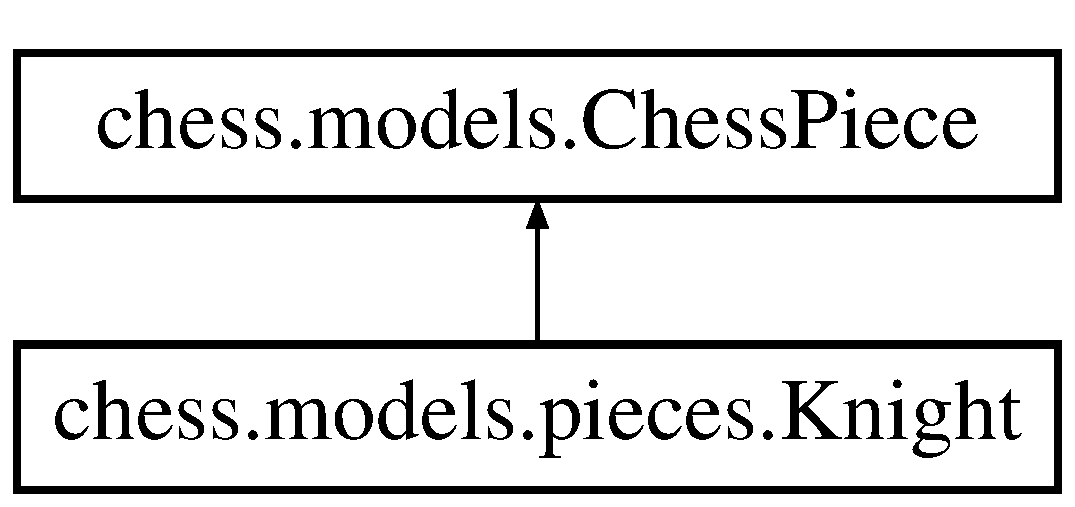
\includegraphics[height=2.000000cm]{classchess_1_1models_1_1pieces_1_1_knight}
\end{center}
\end{figure}
\subsection*{Public Member Functions}
\begin{DoxyCompactItemize}
\item 
\mbox{\hyperlink{classchess_1_1models_1_1pieces_1_1_knight_aa435be794e37d426954f2853a4aac26a}{Knight}} (\mbox{\hyperlink{enumchess_1_1models_1_1enums_1_1_player}{Player}} \mbox{\hyperlink{classchess_1_1models_1_1_chess_piece_a3bcc8a24667318b5aab8c146adcc3eb7}{player}}, \mbox{\hyperlink{classchess_1_1models_1_1_position}{Position}} \mbox{\hyperlink{classchess_1_1models_1_1_chess_piece_a0e4f8616b75e548f269d3971846396f3}{position}})
\item 
\mbox{\hyperlink{enumchess_1_1models_1_1enums_1_1_move_result}{Move\+Result}} \mbox{\hyperlink{classchess_1_1models_1_1pieces_1_1_knight_af1018a686f81f9627d2851c919280448}{is\+Legal\+Move}} (\mbox{\hyperlink{classchess_1_1models_1_1_position}{Position}} pos)
\item 
String \mbox{\hyperlink{classchess_1_1models_1_1pieces_1_1_knight_a18c83fa9040a0035d86c3354f3ada4ea}{to\+String}} ()
\end{DoxyCompactItemize}


\subsection{Detailed Description}
\mbox{\hyperlink{classchess_1_1models_1_1_chess_piece}{Chess\+Piece}} piece\+: \mbox{\hyperlink{classchess_1_1models_1_1pieces_1_1_knight}{Knight}} 

\subsection{Constructor \& Destructor Documentation}
\mbox{\Hypertarget{classchess_1_1models_1_1pieces_1_1_knight_aa435be794e37d426954f2853a4aac26a}\label{classchess_1_1models_1_1pieces_1_1_knight_aa435be794e37d426954f2853a4aac26a}} 
\index{chess\+::models\+::pieces\+::\+Knight@{chess\+::models\+::pieces\+::\+Knight}!Knight@{Knight}}
\index{Knight@{Knight}!chess\+::models\+::pieces\+::\+Knight@{chess\+::models\+::pieces\+::\+Knight}}
\subsubsection{\texorpdfstring{Knight()}{Knight()}}
{\footnotesize\ttfamily chess.\+models.\+pieces.\+Knight.\+Knight (\begin{DoxyParamCaption}\item[{\mbox{\hyperlink{enumchess_1_1models_1_1enums_1_1_player}{Player}}}]{player,  }\item[{\mbox{\hyperlink{classchess_1_1models_1_1_position}{Position}}}]{position }\end{DoxyParamCaption})}

Constructor of \mbox{\hyperlink{classchess_1_1models_1_1pieces_1_1_knight}{Knight}}


\begin{DoxyParams}{Parameters}
{\em player} & Belongs to which player \\
\hline
{\em position} & Initial position \\
\hline
\end{DoxyParams}


\subsection{Member Function Documentation}
\mbox{\Hypertarget{classchess_1_1models_1_1pieces_1_1_knight_af1018a686f81f9627d2851c919280448}\label{classchess_1_1models_1_1pieces_1_1_knight_af1018a686f81f9627d2851c919280448}} 
\index{chess\+::models\+::pieces\+::\+Knight@{chess\+::models\+::pieces\+::\+Knight}!is\+Legal\+Move@{is\+Legal\+Move}}
\index{is\+Legal\+Move@{is\+Legal\+Move}!chess\+::models\+::pieces\+::\+Knight@{chess\+::models\+::pieces\+::\+Knight}}
\subsubsection{\texorpdfstring{is\+Legal\+Move()}{isLegalMove()}}
{\footnotesize\ttfamily \mbox{\hyperlink{enumchess_1_1models_1_1enums_1_1_move_result}{Move\+Result}} chess.\+models.\+pieces.\+Knight.\+is\+Legal\+Move (\begin{DoxyParamCaption}\item[{\mbox{\hyperlink{classchess_1_1models_1_1_position}{Position}}}]{pos }\end{DoxyParamCaption})}

Check if the movement is legal


\begin{DoxyParams}{Parameters}
{\em pos} & Destination position \\
\hline
\end{DoxyParams}
\begin{DoxyReturn}{Returns}
Move\+Result 
\end{DoxyReturn}
\mbox{\Hypertarget{classchess_1_1models_1_1pieces_1_1_knight_a18c83fa9040a0035d86c3354f3ada4ea}\label{classchess_1_1models_1_1pieces_1_1_knight_a18c83fa9040a0035d86c3354f3ada4ea}} 
\index{chess\+::models\+::pieces\+::\+Knight@{chess\+::models\+::pieces\+::\+Knight}!to\+String@{to\+String}}
\index{to\+String@{to\+String}!chess\+::models\+::pieces\+::\+Knight@{chess\+::models\+::pieces\+::\+Knight}}
\subsubsection{\texorpdfstring{to\+String()}{toString()}}
{\footnotesize\ttfamily String chess.\+models.\+pieces.\+Knight.\+to\+String (\begin{DoxyParamCaption}{ }\end{DoxyParamCaption})}



The documentation for this class was generated from the following file\+:\begin{DoxyCompactItemize}
\item 
G\+:/\+Chess/src/main/java/chess/models/pieces/\mbox{\hyperlink{_knight_8java}{Knight.\+java}}\end{DoxyCompactItemize}

\hypertarget{classchess_1_1models_1_1pieces_1_1_knight_test}{}\section{chess.\+models.\+pieces.\+Knight\+Test Class Reference}
\label{classchess_1_1models_1_1pieces_1_1_knight_test}\index{chess.\+models.\+pieces.\+Knight\+Test@{chess.\+models.\+pieces.\+Knight\+Test}}
\subsection*{Public Member Functions}
\begin{DoxyCompactItemize}
\item 
void \mbox{\hyperlink{classchess_1_1models_1_1pieces_1_1_knight_test_a9d4b9c5b54db6a2cb8e161ac8bcf35eb}{is\+Legal\+Move}} ()
\end{DoxyCompactItemize}


\subsection{Member Function Documentation}
\mbox{\Hypertarget{classchess_1_1models_1_1pieces_1_1_knight_test_a9d4b9c5b54db6a2cb8e161ac8bcf35eb}\label{classchess_1_1models_1_1pieces_1_1_knight_test_a9d4b9c5b54db6a2cb8e161ac8bcf35eb}} 
\index{chess\+::models\+::pieces\+::\+Knight\+Test@{chess\+::models\+::pieces\+::\+Knight\+Test}!is\+Legal\+Move@{is\+Legal\+Move}}
\index{is\+Legal\+Move@{is\+Legal\+Move}!chess\+::models\+::pieces\+::\+Knight\+Test@{chess\+::models\+::pieces\+::\+Knight\+Test}}
\subsubsection{\texorpdfstring{is\+Legal\+Move()}{isLegalMove()}}
{\footnotesize\ttfamily void chess.\+models.\+pieces.\+Knight\+Test.\+is\+Legal\+Move (\begin{DoxyParamCaption}{ }\end{DoxyParamCaption})}



The documentation for this class was generated from the following file\+:\begin{DoxyCompactItemize}
\item 
src/test/java/chess/models/pieces/\mbox{\hyperlink{_knight_test_8java}{Knight\+Test.\+java}}\end{DoxyCompactItemize}

\hypertarget{classchess_1_1main_1_1_main}{}\section{chess.\+main.\+Main Class Reference}
\label{classchess_1_1main_1_1_main}\index{chess.\+main.\+Main@{chess.\+main.\+Main}}
Inheritance diagram for chess.\+main.\+Main\+:\begin{figure}[H]
\begin{center}
\leavevmode
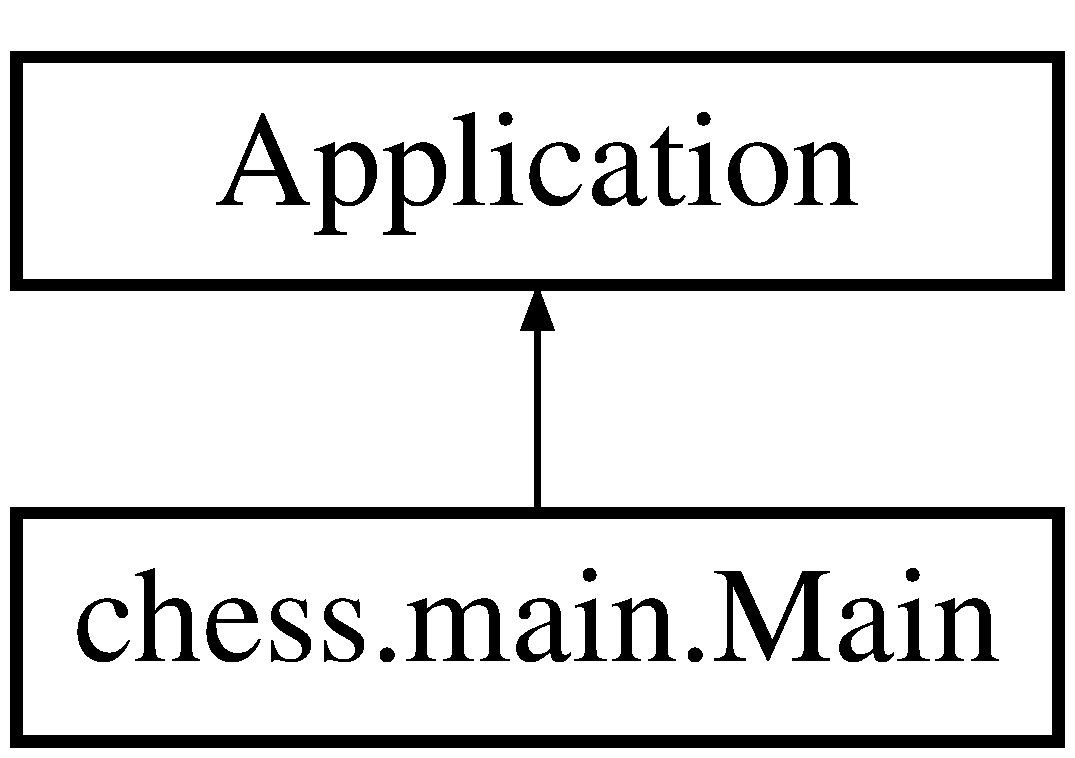
\includegraphics[height=2.000000cm]{classchess_1_1main_1_1_main}
\end{center}
\end{figure}
\subsection*{Public Member Functions}
\begin{DoxyCompactItemize}
\item 
void \mbox{\hyperlink{classchess_1_1main_1_1_main_a673791d4659f12729827e8b279ac83f4}{start}} (Stage primary\+Stage)  throws Exception 
\end{DoxyCompactItemize}
\subsection*{Static Public Member Functions}
\begin{DoxyCompactItemize}
\item 
static void \mbox{\hyperlink{classchess_1_1main_1_1_main_abbdba23121a3431ae17f7df3ee577d10}{main}} (String\mbox{[}$\,$\mbox{]} args)
\end{DoxyCompactItemize}


\subsection{Detailed Description}
\mbox{\hyperlink{classchess_1_1main_1_1_main}{Main}} entrance of the program 

\subsection{Member Function Documentation}
\mbox{\Hypertarget{classchess_1_1main_1_1_main_abbdba23121a3431ae17f7df3ee577d10}\label{classchess_1_1main_1_1_main_abbdba23121a3431ae17f7df3ee577d10}} 
\index{chess\+::main\+::\+Main@{chess\+::main\+::\+Main}!main@{main}}
\index{main@{main}!chess\+::main\+::\+Main@{chess\+::main\+::\+Main}}
\subsubsection{\texorpdfstring{main()}{main()}}
{\footnotesize\ttfamily static void chess.\+main.\+Main.\+main (\begin{DoxyParamCaption}\item[{String \mbox{[}$\,$\mbox{]}}]{args }\end{DoxyParamCaption})\hspace{0.3cm}{\ttfamily [static]}}

\mbox{\Hypertarget{classchess_1_1main_1_1_main_a673791d4659f12729827e8b279ac83f4}\label{classchess_1_1main_1_1_main_a673791d4659f12729827e8b279ac83f4}} 
\index{chess\+::main\+::\+Main@{chess\+::main\+::\+Main}!start@{start}}
\index{start@{start}!chess\+::main\+::\+Main@{chess\+::main\+::\+Main}}
\subsubsection{\texorpdfstring{start()}{start()}}
{\footnotesize\ttfamily void chess.\+main.\+Main.\+start (\begin{DoxyParamCaption}\item[{Stage}]{primary\+Stage }\end{DoxyParamCaption}) throws Exception}



The documentation for this class was generated from the following file\+:\begin{DoxyCompactItemize}
\item 
src/main/java/chess/main/\mbox{\hyperlink{_main_8java}{Main.\+java}}\end{DoxyCompactItemize}

\hypertarget{enumchess_1_1models_1_1enums_1_1_move_result}{}\section{chess.\+models.\+enums.\+Move\+Result Enum Reference}
\label{enumchess_1_1models_1_1enums_1_1_move_result}\index{chess.\+models.\+enums.\+Move\+Result@{chess.\+models.\+enums.\+Move\+Result}}
\subsection*{Public Attributes}
\begin{DoxyCompactItemize}
\item 
\mbox{\hyperlink{enumchess_1_1models_1_1enums_1_1_move_result_aeddb30a26d5d3b05cd22b29ec58b2f2a}{Legal\+Move}}
\item 
\mbox{\hyperlink{enumchess_1_1models_1_1enums_1_1_move_result_ae2f055341a4c6c1c1f3af4437bd0f2d2}{Same\+Position}}
\item 
\mbox{\hyperlink{enumchess_1_1models_1_1enums_1_1_move_result_a683e7b2ca9cb704751385cac155a0cae}{Off\+The\+Board}}
\item 
\mbox{\hyperlink{enumchess_1_1models_1_1enums_1_1_move_result_a4af26e0458f35e2a9c82aa2c27ca134f}{Illegal\+Move}}
\item 
\mbox{\hyperlink{enumchess_1_1models_1_1enums_1_1_move_result_a2717354dfa6f1002293272f66555edcc}{Over\+Other\+Pieces}}
\item 
\mbox{\hyperlink{enumchess_1_1models_1_1enums_1_1_move_result_af4f997ded0a66f0482e263ce6870eba2}{Pawn\+Diagonally}}
\item 
\mbox{\hyperlink{enumchess_1_1models_1_1enums_1_1_move_result_a4f2ef96f4dc4898048a590c502850a54}{Pawn\+Forward}}
\item 
\mbox{\hyperlink{enumchess_1_1models_1_1enums_1_1_move_result_ae617756d07a37d5282a3f680a2dfca3d}{Capture}}
\end{DoxyCompactItemize}


\subsection{Member Data Documentation}
\mbox{\Hypertarget{enumchess_1_1models_1_1enums_1_1_move_result_ae617756d07a37d5282a3f680a2dfca3d}\label{enumchess_1_1models_1_1enums_1_1_move_result_ae617756d07a37d5282a3f680a2dfca3d}} 
\index{chess\+::models\+::enums\+::\+Move\+Result@{chess\+::models\+::enums\+::\+Move\+Result}!Capture@{Capture}}
\index{Capture@{Capture}!chess\+::models\+::enums\+::\+Move\+Result@{chess\+::models\+::enums\+::\+Move\+Result}}
\subsubsection{\texorpdfstring{Capture}{Capture}}
{\footnotesize\ttfamily chess.\+models.\+enums.\+Move\+Result.\+Capture}

\mbox{\Hypertarget{enumchess_1_1models_1_1enums_1_1_move_result_a4af26e0458f35e2a9c82aa2c27ca134f}\label{enumchess_1_1models_1_1enums_1_1_move_result_a4af26e0458f35e2a9c82aa2c27ca134f}} 
\index{chess\+::models\+::enums\+::\+Move\+Result@{chess\+::models\+::enums\+::\+Move\+Result}!Illegal\+Move@{Illegal\+Move}}
\index{Illegal\+Move@{Illegal\+Move}!chess\+::models\+::enums\+::\+Move\+Result@{chess\+::models\+::enums\+::\+Move\+Result}}
\subsubsection{\texorpdfstring{Illegal\+Move}{IllegalMove}}
{\footnotesize\ttfamily chess.\+models.\+enums.\+Move\+Result.\+Illegal\+Move}

\mbox{\Hypertarget{enumchess_1_1models_1_1enums_1_1_move_result_aeddb30a26d5d3b05cd22b29ec58b2f2a}\label{enumchess_1_1models_1_1enums_1_1_move_result_aeddb30a26d5d3b05cd22b29ec58b2f2a}} 
\index{chess\+::models\+::enums\+::\+Move\+Result@{chess\+::models\+::enums\+::\+Move\+Result}!Legal\+Move@{Legal\+Move}}
\index{Legal\+Move@{Legal\+Move}!chess\+::models\+::enums\+::\+Move\+Result@{chess\+::models\+::enums\+::\+Move\+Result}}
\subsubsection{\texorpdfstring{Legal\+Move}{LegalMove}}
{\footnotesize\ttfamily chess.\+models.\+enums.\+Move\+Result.\+Legal\+Move}

\mbox{\Hypertarget{enumchess_1_1models_1_1enums_1_1_move_result_a683e7b2ca9cb704751385cac155a0cae}\label{enumchess_1_1models_1_1enums_1_1_move_result_a683e7b2ca9cb704751385cac155a0cae}} 
\index{chess\+::models\+::enums\+::\+Move\+Result@{chess\+::models\+::enums\+::\+Move\+Result}!Off\+The\+Board@{Off\+The\+Board}}
\index{Off\+The\+Board@{Off\+The\+Board}!chess\+::models\+::enums\+::\+Move\+Result@{chess\+::models\+::enums\+::\+Move\+Result}}
\subsubsection{\texorpdfstring{Off\+The\+Board}{OffTheBoard}}
{\footnotesize\ttfamily chess.\+models.\+enums.\+Move\+Result.\+Off\+The\+Board}

\mbox{\Hypertarget{enumchess_1_1models_1_1enums_1_1_move_result_a2717354dfa6f1002293272f66555edcc}\label{enumchess_1_1models_1_1enums_1_1_move_result_a2717354dfa6f1002293272f66555edcc}} 
\index{chess\+::models\+::enums\+::\+Move\+Result@{chess\+::models\+::enums\+::\+Move\+Result}!Over\+Other\+Pieces@{Over\+Other\+Pieces}}
\index{Over\+Other\+Pieces@{Over\+Other\+Pieces}!chess\+::models\+::enums\+::\+Move\+Result@{chess\+::models\+::enums\+::\+Move\+Result}}
\subsubsection{\texorpdfstring{Over\+Other\+Pieces}{OverOtherPieces}}
{\footnotesize\ttfamily chess.\+models.\+enums.\+Move\+Result.\+Over\+Other\+Pieces}

\mbox{\Hypertarget{enumchess_1_1models_1_1enums_1_1_move_result_af4f997ded0a66f0482e263ce6870eba2}\label{enumchess_1_1models_1_1enums_1_1_move_result_af4f997ded0a66f0482e263ce6870eba2}} 
\index{chess\+::models\+::enums\+::\+Move\+Result@{chess\+::models\+::enums\+::\+Move\+Result}!Pawn\+Diagonally@{Pawn\+Diagonally}}
\index{Pawn\+Diagonally@{Pawn\+Diagonally}!chess\+::models\+::enums\+::\+Move\+Result@{chess\+::models\+::enums\+::\+Move\+Result}}
\subsubsection{\texorpdfstring{Pawn\+Diagonally}{PawnDiagonally}}
{\footnotesize\ttfamily chess.\+models.\+enums.\+Move\+Result.\+Pawn\+Diagonally}

\mbox{\Hypertarget{enumchess_1_1models_1_1enums_1_1_move_result_a4f2ef96f4dc4898048a590c502850a54}\label{enumchess_1_1models_1_1enums_1_1_move_result_a4f2ef96f4dc4898048a590c502850a54}} 
\index{chess\+::models\+::enums\+::\+Move\+Result@{chess\+::models\+::enums\+::\+Move\+Result}!Pawn\+Forward@{Pawn\+Forward}}
\index{Pawn\+Forward@{Pawn\+Forward}!chess\+::models\+::enums\+::\+Move\+Result@{chess\+::models\+::enums\+::\+Move\+Result}}
\subsubsection{\texorpdfstring{Pawn\+Forward}{PawnForward}}
{\footnotesize\ttfamily chess.\+models.\+enums.\+Move\+Result.\+Pawn\+Forward}

\mbox{\Hypertarget{enumchess_1_1models_1_1enums_1_1_move_result_ae2f055341a4c6c1c1f3af4437bd0f2d2}\label{enumchess_1_1models_1_1enums_1_1_move_result_ae2f055341a4c6c1c1f3af4437bd0f2d2}} 
\index{chess\+::models\+::enums\+::\+Move\+Result@{chess\+::models\+::enums\+::\+Move\+Result}!Same\+Position@{Same\+Position}}
\index{Same\+Position@{Same\+Position}!chess\+::models\+::enums\+::\+Move\+Result@{chess\+::models\+::enums\+::\+Move\+Result}}
\subsubsection{\texorpdfstring{Same\+Position}{SamePosition}}
{\footnotesize\ttfamily chess.\+models.\+enums.\+Move\+Result.\+Same\+Position}



The documentation for this enum was generated from the following file\+:\begin{DoxyCompactItemize}
\item 
src/main/java/chess/models/enums/\mbox{\hyperlink{_move_result_8java}{Move\+Result.\+java}}\end{DoxyCompactItemize}

\hypertarget{classchess_1_1models_1_1_path}{}\section{chess.\+models.\+Path Class Reference}
\label{classchess_1_1models_1_1_path}\index{chess.\+models.\+Path@{chess.\+models.\+Path}}
\subsection*{Public Member Functions}
\begin{DoxyCompactItemize}
\item 
\mbox{\hyperlink{classchess_1_1models_1_1_path_a5ddc0a03cb1c2b1dd93f77dbecfcdc27}{Path}} (\mbox{\hyperlink{classchess_1_1models_1_1_position}{Position}} pos1, \mbox{\hyperlink{classchess_1_1models_1_1_position}{Position}} pos2)
\item 
Set$<$ \mbox{\hyperlink{classchess_1_1models_1_1_position}{Position}} $>$ \mbox{\hyperlink{classchess_1_1models_1_1_path_adce43d0b62fd3ba9d7ac261fcf4cf7b1}{get\+Positions}} ()
\end{DoxyCompactItemize}
\subsection*{Private Attributes}
\begin{DoxyCompactItemize}
\item 
Set$<$ \mbox{\hyperlink{classchess_1_1models_1_1_position}{Position}} $>$ \mbox{\hyperlink{classchess_1_1models_1_1_path_abfd1faa7caf599ad3d8a2a0fa03ee883}{positions}}
\end{DoxyCompactItemize}


\subsection{Detailed Description}
\mbox{\hyperlink{classchess_1_1models_1_1_path}{Path}} between two positions. 

\subsection{Constructor \& Destructor Documentation}
\mbox{\Hypertarget{classchess_1_1models_1_1_path_a5ddc0a03cb1c2b1dd93f77dbecfcdc27}\label{classchess_1_1models_1_1_path_a5ddc0a03cb1c2b1dd93f77dbecfcdc27}} 
\index{chess\+::models\+::\+Path@{chess\+::models\+::\+Path}!Path@{Path}}
\index{Path@{Path}!chess\+::models\+::\+Path@{chess\+::models\+::\+Path}}
\subsubsection{\texorpdfstring{Path()}{Path()}}
{\footnotesize\ttfamily chess.\+models.\+Path.\+Path (\begin{DoxyParamCaption}\item[{\mbox{\hyperlink{classchess_1_1models_1_1_position}{Position}}}]{pos1,  }\item[{\mbox{\hyperlink{classchess_1_1models_1_1_position}{Position}}}]{pos2 }\end{DoxyParamCaption})}

Constructor of \mbox{\hyperlink{classchess_1_1models_1_1_path}{Path}}


\begin{DoxyParams}{Parameters}
{\em pos1} & One of the end points of the path \\
\hline
{\em pos2} & the ohter end point of the path \\
\hline
\end{DoxyParams}


\subsection{Member Function Documentation}
\mbox{\Hypertarget{classchess_1_1models_1_1_path_adce43d0b62fd3ba9d7ac261fcf4cf7b1}\label{classchess_1_1models_1_1_path_adce43d0b62fd3ba9d7ac261fcf4cf7b1}} 
\index{chess\+::models\+::\+Path@{chess\+::models\+::\+Path}!get\+Positions@{get\+Positions}}
\index{get\+Positions@{get\+Positions}!chess\+::models\+::\+Path@{chess\+::models\+::\+Path}}
\subsubsection{\texorpdfstring{get\+Positions()}{getPositions()}}
{\footnotesize\ttfamily Set$<$\mbox{\hyperlink{classchess_1_1models_1_1_position}{Position}}$>$ chess.\+models.\+Path.\+get\+Positions (\begin{DoxyParamCaption}{ }\end{DoxyParamCaption})}

Get all positions on the path

\begin{DoxyReturn}{Returns}
all positions on the path 
\end{DoxyReturn}


\subsection{Member Data Documentation}
\mbox{\Hypertarget{classchess_1_1models_1_1_path_abfd1faa7caf599ad3d8a2a0fa03ee883}\label{classchess_1_1models_1_1_path_abfd1faa7caf599ad3d8a2a0fa03ee883}} 
\index{chess\+::models\+::\+Path@{chess\+::models\+::\+Path}!positions@{positions}}
\index{positions@{positions}!chess\+::models\+::\+Path@{chess\+::models\+::\+Path}}
\subsubsection{\texorpdfstring{positions}{positions}}
{\footnotesize\ttfamily Set$<$\mbox{\hyperlink{classchess_1_1models_1_1_position}{Position}}$>$ chess.\+models.\+Path.\+positions\hspace{0.3cm}{\ttfamily [private]}}



The documentation for this class was generated from the following file\+:\begin{DoxyCompactItemize}
\item 
G\+:/\+Chess/src/main/java/chess/models/\mbox{\hyperlink{_path_8java}{Path.\+java}}\end{DoxyCompactItemize}

\hypertarget{classchess_1_1models_1_1_path_test}{}\section{chess.\+models.\+Path\+Test Class Reference}
\label{classchess_1_1models_1_1_path_test}\index{chess.\+models.\+Path\+Test@{chess.\+models.\+Path\+Test}}
\subsection*{Public Member Functions}
\begin{DoxyCompactItemize}
\item 
void \mbox{\hyperlink{classchess_1_1models_1_1_path_test_af8658336e6ffed8c20de620ad12a37e3}{get\+Positions1}} ()
\item 
void \mbox{\hyperlink{classchess_1_1models_1_1_path_test_a572cc15adf7eb579533b04040f14fc41}{get\+Positions2}} ()
\item 
void \mbox{\hyperlink{classchess_1_1models_1_1_path_test_a42e6278bdbd086dbb1394c8bf873a0af}{get\+Positions3}} ()
\item 
boolean \mbox{\hyperlink{classchess_1_1models_1_1_path_test_a6c2cec1f3d389067e84ff5fe93a6b6a8}{is\+Set\+Equals}} (Set$<$ \mbox{\hyperlink{classchess_1_1models_1_1_position}{Position}} $>$ expected\+Pos\+Set, Set$<$ \mbox{\hyperlink{classchess_1_1models_1_1_position}{Position}} $>$ actual\+Pos\+Set)
\end{DoxyCompactItemize}


\subsection{Member Function Documentation}
\mbox{\Hypertarget{classchess_1_1models_1_1_path_test_af8658336e6ffed8c20de620ad12a37e3}\label{classchess_1_1models_1_1_path_test_af8658336e6ffed8c20de620ad12a37e3}} 
\index{chess\+::models\+::\+Path\+Test@{chess\+::models\+::\+Path\+Test}!get\+Positions1@{get\+Positions1}}
\index{get\+Positions1@{get\+Positions1}!chess\+::models\+::\+Path\+Test@{chess\+::models\+::\+Path\+Test}}
\subsubsection{\texorpdfstring{get\+Positions1()}{getPositions1()}}
{\footnotesize\ttfamily void chess.\+models.\+Path\+Test.\+get\+Positions1 (\begin{DoxyParamCaption}{ }\end{DoxyParamCaption})}

Method\+: get\+Positions() \mbox{\Hypertarget{classchess_1_1models_1_1_path_test_a572cc15adf7eb579533b04040f14fc41}\label{classchess_1_1models_1_1_path_test_a572cc15adf7eb579533b04040f14fc41}} 
\index{chess\+::models\+::\+Path\+Test@{chess\+::models\+::\+Path\+Test}!get\+Positions2@{get\+Positions2}}
\index{get\+Positions2@{get\+Positions2}!chess\+::models\+::\+Path\+Test@{chess\+::models\+::\+Path\+Test}}
\subsubsection{\texorpdfstring{get\+Positions2()}{getPositions2()}}
{\footnotesize\ttfamily void chess.\+models.\+Path\+Test.\+get\+Positions2 (\begin{DoxyParamCaption}{ }\end{DoxyParamCaption})}

\mbox{\Hypertarget{classchess_1_1models_1_1_path_test_a42e6278bdbd086dbb1394c8bf873a0af}\label{classchess_1_1models_1_1_path_test_a42e6278bdbd086dbb1394c8bf873a0af}} 
\index{chess\+::models\+::\+Path\+Test@{chess\+::models\+::\+Path\+Test}!get\+Positions3@{get\+Positions3}}
\index{get\+Positions3@{get\+Positions3}!chess\+::models\+::\+Path\+Test@{chess\+::models\+::\+Path\+Test}}
\subsubsection{\texorpdfstring{get\+Positions3()}{getPositions3()}}
{\footnotesize\ttfamily void chess.\+models.\+Path\+Test.\+get\+Positions3 (\begin{DoxyParamCaption}{ }\end{DoxyParamCaption})}

\mbox{\Hypertarget{classchess_1_1models_1_1_path_test_a6c2cec1f3d389067e84ff5fe93a6b6a8}\label{classchess_1_1models_1_1_path_test_a6c2cec1f3d389067e84ff5fe93a6b6a8}} 
\index{chess\+::models\+::\+Path\+Test@{chess\+::models\+::\+Path\+Test}!is\+Set\+Equals@{is\+Set\+Equals}}
\index{is\+Set\+Equals@{is\+Set\+Equals}!chess\+::models\+::\+Path\+Test@{chess\+::models\+::\+Path\+Test}}
\subsubsection{\texorpdfstring{is\+Set\+Equals()}{isSetEquals()}}
{\footnotesize\ttfamily boolean chess.\+models.\+Path\+Test.\+is\+Set\+Equals (\begin{DoxyParamCaption}\item[{Set$<$ \mbox{\hyperlink{classchess_1_1models_1_1_position}{Position}} $>$}]{expected\+Pos\+Set,  }\item[{Set$<$ \mbox{\hyperlink{classchess_1_1models_1_1_position}{Position}} $>$}]{actual\+Pos\+Set }\end{DoxyParamCaption})}



The documentation for this class was generated from the following file\+:\begin{DoxyCompactItemize}
\item 
G\+:/\+Chess/src/test/java/chess/models/\mbox{\hyperlink{_path_test_8java}{Path\+Test.\+java}}\end{DoxyCompactItemize}

\hypertarget{classchess_1_1models_1_1pieces_1_1_pawn}{}\section{chess.\+models.\+pieces.\+Pawn Class Reference}
\label{classchess_1_1models_1_1pieces_1_1_pawn}\index{chess.\+models.\+pieces.\+Pawn@{chess.\+models.\+pieces.\+Pawn}}
Inheritance diagram for chess.\+models.\+pieces.\+Pawn\+:\begin{figure}[H]
\begin{center}
\leavevmode
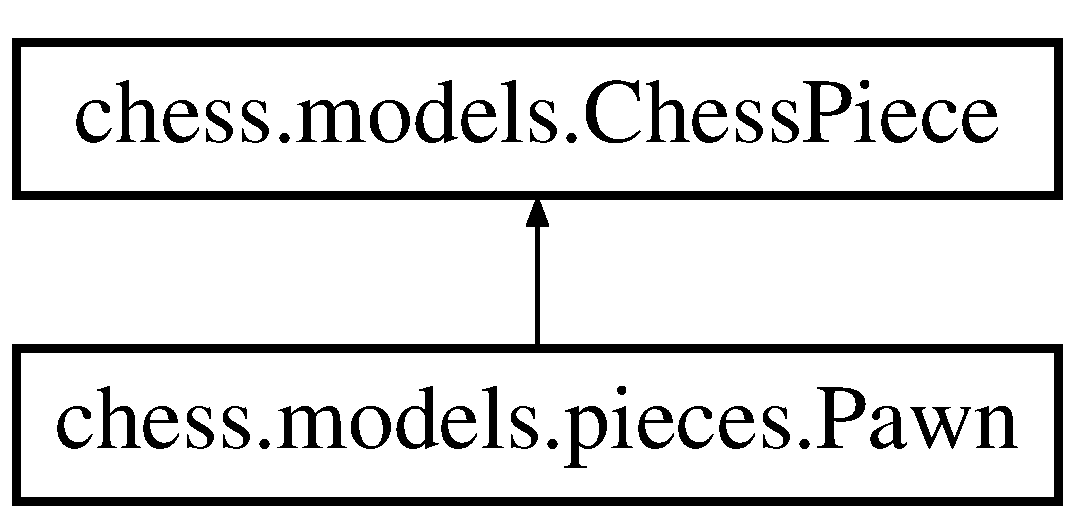
\includegraphics[height=2.000000cm]{classchess_1_1models_1_1pieces_1_1_pawn}
\end{center}
\end{figure}
\subsection*{Public Member Functions}
\begin{DoxyCompactItemize}
\item 
\mbox{\hyperlink{classchess_1_1models_1_1pieces_1_1_pawn_aa62632674360fd0518f583bf1477b8c1}{Pawn}} (\mbox{\hyperlink{enumchess_1_1models_1_1enums_1_1_player}{Player}} \mbox{\hyperlink{classchess_1_1models_1_1_chess_piece_a3bcc8a24667318b5aab8c146adcc3eb7}{player}}, \mbox{\hyperlink{classchess_1_1models_1_1_position}{Position}} \mbox{\hyperlink{classchess_1_1models_1_1_chess_piece_a0e4f8616b75e548f269d3971846396f3}{position}})
\item 
\mbox{\hyperlink{enumchess_1_1models_1_1enums_1_1_move_result}{Move\+Result}} \mbox{\hyperlink{classchess_1_1models_1_1pieces_1_1_pawn_ae293ed0d437de535ad14a543a1077871}{is\+Legal\+Move}} (\mbox{\hyperlink{classchess_1_1models_1_1_position}{Position}} pos)
\item 
boolean \mbox{\hyperlink{classchess_1_1models_1_1pieces_1_1_pawn_a80055e2b99a160f4de32644423460a6f}{is\+Forward}} (\mbox{\hyperlink{classchess_1_1models_1_1_position}{Position}} pos)
\item 
String \mbox{\hyperlink{classchess_1_1models_1_1pieces_1_1_pawn_a97538699aaa1cb69482ad9c218562450}{to\+String}} ()
\item 
void \mbox{\hyperlink{classchess_1_1models_1_1pieces_1_1_pawn_afb8291b2ab13822506cccad5dbe8fc91}{move}} (\mbox{\hyperlink{classchess_1_1models_1_1_position}{Position}} pos)
\end{DoxyCompactItemize}
\subsection*{Private Attributes}
\begin{DoxyCompactItemize}
\item 
boolean \mbox{\hyperlink{classchess_1_1models_1_1pieces_1_1_pawn_a450300d4ee1338fa478c717a345dd82c}{is\+First\+Step}}
\end{DoxyCompactItemize}


\subsection{Detailed Description}
\mbox{\hyperlink{classchess_1_1models_1_1_chess_piece}{Chess\+Piece}} piece\+: \mbox{\hyperlink{classchess_1_1models_1_1pieces_1_1_pawn}{Pawn}} 

\subsection{Constructor \& Destructor Documentation}
\mbox{\Hypertarget{classchess_1_1models_1_1pieces_1_1_pawn_aa62632674360fd0518f583bf1477b8c1}\label{classchess_1_1models_1_1pieces_1_1_pawn_aa62632674360fd0518f583bf1477b8c1}} 
\index{chess\+::models\+::pieces\+::\+Pawn@{chess\+::models\+::pieces\+::\+Pawn}!Pawn@{Pawn}}
\index{Pawn@{Pawn}!chess\+::models\+::pieces\+::\+Pawn@{chess\+::models\+::pieces\+::\+Pawn}}
\subsubsection{\texorpdfstring{Pawn()}{Pawn()}}
{\footnotesize\ttfamily chess.\+models.\+pieces.\+Pawn.\+Pawn (\begin{DoxyParamCaption}\item[{\mbox{\hyperlink{enumchess_1_1models_1_1enums_1_1_player}{Player}}}]{player,  }\item[{\mbox{\hyperlink{classchess_1_1models_1_1_position}{Position}}}]{position }\end{DoxyParamCaption})}

Constructor of \mbox{\hyperlink{classchess_1_1models_1_1pieces_1_1_pawn}{Pawn}}


\begin{DoxyParams}{Parameters}
{\em player} & Belongs to which player \\
\hline
{\em position} & Initial position \\
\hline
\end{DoxyParams}


\subsection{Member Function Documentation}
\mbox{\Hypertarget{classchess_1_1models_1_1pieces_1_1_pawn_a80055e2b99a160f4de32644423460a6f}\label{classchess_1_1models_1_1pieces_1_1_pawn_a80055e2b99a160f4de32644423460a6f}} 
\index{chess\+::models\+::pieces\+::\+Pawn@{chess\+::models\+::pieces\+::\+Pawn}!is\+Forward@{is\+Forward}}
\index{is\+Forward@{is\+Forward}!chess\+::models\+::pieces\+::\+Pawn@{chess\+::models\+::pieces\+::\+Pawn}}
\subsubsection{\texorpdfstring{is\+Forward()}{isForward()}}
{\footnotesize\ttfamily boolean chess.\+models.\+pieces.\+Pawn.\+is\+Forward (\begin{DoxyParamCaption}\item[{\mbox{\hyperlink{classchess_1_1models_1_1_position}{Position}}}]{pos }\end{DoxyParamCaption})}

Check if the pawn is moving forward


\begin{DoxyParams}{Parameters}
{\em pos} & Destination position \\
\hline
\end{DoxyParams}
\begin{DoxyReturn}{Returns}
true is that the pawn is moving forward 
\end{DoxyReturn}
\mbox{\Hypertarget{classchess_1_1models_1_1pieces_1_1_pawn_ae293ed0d437de535ad14a543a1077871}\label{classchess_1_1models_1_1pieces_1_1_pawn_ae293ed0d437de535ad14a543a1077871}} 
\index{chess\+::models\+::pieces\+::\+Pawn@{chess\+::models\+::pieces\+::\+Pawn}!is\+Legal\+Move@{is\+Legal\+Move}}
\index{is\+Legal\+Move@{is\+Legal\+Move}!chess\+::models\+::pieces\+::\+Pawn@{chess\+::models\+::pieces\+::\+Pawn}}
\subsubsection{\texorpdfstring{is\+Legal\+Move()}{isLegalMove()}}
{\footnotesize\ttfamily \mbox{\hyperlink{enumchess_1_1models_1_1enums_1_1_move_result}{Move\+Result}} chess.\+models.\+pieces.\+Pawn.\+is\+Legal\+Move (\begin{DoxyParamCaption}\item[{\mbox{\hyperlink{classchess_1_1models_1_1_position}{Position}}}]{pos }\end{DoxyParamCaption})}

Check if the movement is legal


\begin{DoxyParams}{Parameters}
{\em pos} & Destination position \\
\hline
\end{DoxyParams}
\begin{DoxyReturn}{Returns}
Move\+Result 
\end{DoxyReturn}
\mbox{\Hypertarget{classchess_1_1models_1_1pieces_1_1_pawn_afb8291b2ab13822506cccad5dbe8fc91}\label{classchess_1_1models_1_1pieces_1_1_pawn_afb8291b2ab13822506cccad5dbe8fc91}} 
\index{chess\+::models\+::pieces\+::\+Pawn@{chess\+::models\+::pieces\+::\+Pawn}!move@{move}}
\index{move@{move}!chess\+::models\+::pieces\+::\+Pawn@{chess\+::models\+::pieces\+::\+Pawn}}
\subsubsection{\texorpdfstring{move()}{move()}}
{\footnotesize\ttfamily void chess.\+models.\+pieces.\+Pawn.\+move (\begin{DoxyParamCaption}\item[{\mbox{\hyperlink{classchess_1_1models_1_1_position}{Position}}}]{pos }\end{DoxyParamCaption})}

\mbox{\Hypertarget{classchess_1_1models_1_1pieces_1_1_pawn_a97538699aaa1cb69482ad9c218562450}\label{classchess_1_1models_1_1pieces_1_1_pawn_a97538699aaa1cb69482ad9c218562450}} 
\index{chess\+::models\+::pieces\+::\+Pawn@{chess\+::models\+::pieces\+::\+Pawn}!to\+String@{to\+String}}
\index{to\+String@{to\+String}!chess\+::models\+::pieces\+::\+Pawn@{chess\+::models\+::pieces\+::\+Pawn}}
\subsubsection{\texorpdfstring{to\+String()}{toString()}}
{\footnotesize\ttfamily String chess.\+models.\+pieces.\+Pawn.\+to\+String (\begin{DoxyParamCaption}{ }\end{DoxyParamCaption})}



\subsection{Member Data Documentation}
\mbox{\Hypertarget{classchess_1_1models_1_1pieces_1_1_pawn_a450300d4ee1338fa478c717a345dd82c}\label{classchess_1_1models_1_1pieces_1_1_pawn_a450300d4ee1338fa478c717a345dd82c}} 
\index{chess\+::models\+::pieces\+::\+Pawn@{chess\+::models\+::pieces\+::\+Pawn}!is\+First\+Step@{is\+First\+Step}}
\index{is\+First\+Step@{is\+First\+Step}!chess\+::models\+::pieces\+::\+Pawn@{chess\+::models\+::pieces\+::\+Pawn}}
\subsubsection{\texorpdfstring{is\+First\+Step}{isFirstStep}}
{\footnotesize\ttfamily boolean chess.\+models.\+pieces.\+Pawn.\+is\+First\+Step\hspace{0.3cm}{\ttfamily [private]}}



The documentation for this class was generated from the following file\+:\begin{DoxyCompactItemize}
\item 
G\+:/\+Chess/src/main/java/chess/models/pieces/\mbox{\hyperlink{_pawn_8java}{Pawn.\+java}}\end{DoxyCompactItemize}

\hypertarget{classchess_1_1models_1_1pieces_1_1_pawn_test}{}\section{chess.\+models.\+pieces.\+Pawn\+Test Class Reference}
\label{classchess_1_1models_1_1pieces_1_1_pawn_test}\index{chess.\+models.\+pieces.\+Pawn\+Test@{chess.\+models.\+pieces.\+Pawn\+Test}}
\subsection*{Public Member Functions}
\begin{DoxyCompactItemize}
\item 
void \mbox{\hyperlink{classchess_1_1models_1_1pieces_1_1_pawn_test_afa43463ef4516891aa999190df961e1e}{is\+Forward}} ()
\item 
void \mbox{\hyperlink{classchess_1_1models_1_1pieces_1_1_pawn_test_a27e7deb43705ed5723795f0b9aa8ea9a}{is\+Legal\+Move}} ()
\end{DoxyCompactItemize}


\subsection{Member Function Documentation}
\mbox{\Hypertarget{classchess_1_1models_1_1pieces_1_1_pawn_test_afa43463ef4516891aa999190df961e1e}\label{classchess_1_1models_1_1pieces_1_1_pawn_test_afa43463ef4516891aa999190df961e1e}} 
\index{chess\+::models\+::pieces\+::\+Pawn\+Test@{chess\+::models\+::pieces\+::\+Pawn\+Test}!is\+Forward@{is\+Forward}}
\index{is\+Forward@{is\+Forward}!chess\+::models\+::pieces\+::\+Pawn\+Test@{chess\+::models\+::pieces\+::\+Pawn\+Test}}
\subsubsection{\texorpdfstring{is\+Forward()}{isForward()}}
{\footnotesize\ttfamily void chess.\+models.\+pieces.\+Pawn\+Test.\+is\+Forward (\begin{DoxyParamCaption}{ }\end{DoxyParamCaption})}

\mbox{\Hypertarget{classchess_1_1models_1_1pieces_1_1_pawn_test_a27e7deb43705ed5723795f0b9aa8ea9a}\label{classchess_1_1models_1_1pieces_1_1_pawn_test_a27e7deb43705ed5723795f0b9aa8ea9a}} 
\index{chess\+::models\+::pieces\+::\+Pawn\+Test@{chess\+::models\+::pieces\+::\+Pawn\+Test}!is\+Legal\+Move@{is\+Legal\+Move}}
\index{is\+Legal\+Move@{is\+Legal\+Move}!chess\+::models\+::pieces\+::\+Pawn\+Test@{chess\+::models\+::pieces\+::\+Pawn\+Test}}
\subsubsection{\texorpdfstring{is\+Legal\+Move()}{isLegalMove()}}
{\footnotesize\ttfamily void chess.\+models.\+pieces.\+Pawn\+Test.\+is\+Legal\+Move (\begin{DoxyParamCaption}{ }\end{DoxyParamCaption})}



The documentation for this class was generated from the following file\+:\begin{DoxyCompactItemize}
\item 
src/test/java/chess/models/pieces/\mbox{\hyperlink{_pawn_test_8java}{Pawn\+Test.\+java}}\end{DoxyCompactItemize}

\hypertarget{enumchess_1_1models_1_1enums_1_1_player}{}\section{chess.\+models.\+enums.\+Player Enum Reference}
\label{enumchess_1_1models_1_1enums_1_1_player}\index{chess.\+models.\+enums.\+Player@{chess.\+models.\+enums.\+Player}}
\subsection*{Public Attributes}
\begin{DoxyCompactItemize}
\item 
\mbox{\hyperlink{enumchess_1_1models_1_1enums_1_1_player_a37677111d3c5ecaf7109ebe257b7d756}{Black}}
\item 
\mbox{\hyperlink{enumchess_1_1models_1_1enums_1_1_player_a60ced79fc80ec46a6a2a6f031b27b08e}{White}}
\end{DoxyCompactItemize}


\subsection{Member Data Documentation}
\mbox{\Hypertarget{enumchess_1_1models_1_1enums_1_1_player_a37677111d3c5ecaf7109ebe257b7d756}\label{enumchess_1_1models_1_1enums_1_1_player_a37677111d3c5ecaf7109ebe257b7d756}} 
\index{chess\+::models\+::enums\+::\+Player@{chess\+::models\+::enums\+::\+Player}!Black@{Black}}
\index{Black@{Black}!chess\+::models\+::enums\+::\+Player@{chess\+::models\+::enums\+::\+Player}}
\subsubsection{\texorpdfstring{Black}{Black}}
{\footnotesize\ttfamily chess.\+models.\+enums.\+Player.\+Black}

\mbox{\Hypertarget{enumchess_1_1models_1_1enums_1_1_player_a60ced79fc80ec46a6a2a6f031b27b08e}\label{enumchess_1_1models_1_1enums_1_1_player_a60ced79fc80ec46a6a2a6f031b27b08e}} 
\index{chess\+::models\+::enums\+::\+Player@{chess\+::models\+::enums\+::\+Player}!White@{White}}
\index{White@{White}!chess\+::models\+::enums\+::\+Player@{chess\+::models\+::enums\+::\+Player}}
\subsubsection{\texorpdfstring{White}{White}}
{\footnotesize\ttfamily chess.\+models.\+enums.\+Player.\+White}



The documentation for this enum was generated from the following file\+:\begin{DoxyCompactItemize}
\item 
G\+:/\+Chess/src/main/java/chess/models/enums/\mbox{\hyperlink{_player_8java}{Player.\+java}}\end{DoxyCompactItemize}

\hypertarget{classchess_1_1models_1_1_position}{}\section{chess.\+models.\+Position Class Reference}
\label{classchess_1_1models_1_1_position}\index{chess.\+models.\+Position@{chess.\+models.\+Position}}
\subsection*{Public Member Functions}
\begin{DoxyCompactItemize}
\item 
\mbox{\hyperlink{classchess_1_1models_1_1_position_af2ca0e2b74a18503f08e8492a52501c1}{Position}} (String position)
\item 
\mbox{\hyperlink{classchess_1_1models_1_1_position_aa5e15407a249f22ba683d43083c3f16b}{Position}} (int x, int y)
\item 
int \mbox{\hyperlink{classchess_1_1models_1_1_position_a1de14ed4ac5e2376caf3ecbf4f415e38}{getX}} ()
\item 
int \mbox{\hyperlink{classchess_1_1models_1_1_position_aa4cdabf057a4a9fac849b04dc687a8ed}{getY}} ()
\item 
boolean \mbox{\hyperlink{classchess_1_1models_1_1_position_ab66e53b6cb98e557aa0fc811e7987486}{equals}} (\mbox{\hyperlink{classchess_1_1models_1_1_position}{Position}} pos)
\item 
int \mbox{\hyperlink{classchess_1_1models_1_1_position_ad2ac6e3457056ccba6f1ccf3603f2554}{distance}} (\mbox{\hyperlink{classchess_1_1models_1_1_position}{Position}} pos)
\item 
boolean \mbox{\hyperlink{classchess_1_1models_1_1_position_a5fdc417a5c9eed00af982d202b505767}{is\+Horizontal}} (\mbox{\hyperlink{classchess_1_1models_1_1_position}{Position}} pos)
\item 
boolean \mbox{\hyperlink{classchess_1_1models_1_1_position_a50da6933e82356a80b6f012251189d25}{is\+Vertical}} (\mbox{\hyperlink{classchess_1_1models_1_1_position}{Position}} pos)
\item 
boolean \mbox{\hyperlink{classchess_1_1models_1_1_position_a359f1be865e9ba19dc94116ce1fe8214}{is\+Diagonal}} (\mbox{\hyperlink{classchess_1_1models_1_1_position}{Position}} pos)
\item 
boolean \mbox{\hyperlink{classchess_1_1models_1_1_position_a7e79c1169c4333aa98d6445af82ea5e2}{is\+L\+Shape}} (\mbox{\hyperlink{classchess_1_1models_1_1_position}{Position}} pos)
\item 
List$<$ \mbox{\hyperlink{classchess_1_1models_1_1_position}{Position}} $>$ \mbox{\hyperlink{classchess_1_1models_1_1_position_a86f1df8c1f1a5303a0bb0386c5181eef}{around\+Pos}} ()
\end{DoxyCompactItemize}


\subsection{Detailed Description}
\mbox{\hyperlink{classchess_1_1models_1_1_position}{Position}} of chess pieces on the board 

\subsection{Constructor \& Destructor Documentation}
\mbox{\Hypertarget{classchess_1_1models_1_1_position_af2ca0e2b74a18503f08e8492a52501c1}\label{classchess_1_1models_1_1_position_af2ca0e2b74a18503f08e8492a52501c1}} 
\index{chess\+::models\+::\+Position@{chess\+::models\+::\+Position}!Position@{Position}}
\index{Position@{Position}!chess\+::models\+::\+Position@{chess\+::models\+::\+Position}}
\subsubsection{\texorpdfstring{Position()}{Position()}\hspace{0.1cm}{\footnotesize\ttfamily [1/2]}}
{\footnotesize\ttfamily chess.\+models.\+Position.\+Position (\begin{DoxyParamCaption}\item[{String}]{position }\end{DoxyParamCaption})}

Constructor of \mbox{\hyperlink{classchess_1_1models_1_1_position}{Position}}


\begin{DoxyParams}{Parameters}
{\em position} & \mbox{\hyperlink{classchess_1_1models_1_1_position}{Position}} in string format, such as \char`\"{}\+A4\char`\"{}, \char`\"{}\+E6\char`\"{} \\
\hline
\end{DoxyParams}
\mbox{\Hypertarget{classchess_1_1models_1_1_position_aa5e15407a249f22ba683d43083c3f16b}\label{classchess_1_1models_1_1_position_aa5e15407a249f22ba683d43083c3f16b}} 
\index{chess\+::models\+::\+Position@{chess\+::models\+::\+Position}!Position@{Position}}
\index{Position@{Position}!chess\+::models\+::\+Position@{chess\+::models\+::\+Position}}
\subsubsection{\texorpdfstring{Position()}{Position()}\hspace{0.1cm}{\footnotesize\ttfamily [2/2]}}
{\footnotesize\ttfamily chess.\+models.\+Position.\+Position (\begin{DoxyParamCaption}\item[{int}]{x,  }\item[{int}]{y }\end{DoxyParamCaption})}

Constructor of \mbox{\hyperlink{classchess_1_1models_1_1_position}{Position}}


\begin{DoxyParams}{Parameters}
{\em x} & Horizontal position \\
\hline
{\em y} & Vertical position \\
\hline
\end{DoxyParams}


\subsection{Member Function Documentation}
\mbox{\Hypertarget{classchess_1_1models_1_1_position_a86f1df8c1f1a5303a0bb0386c5181eef}\label{classchess_1_1models_1_1_position_a86f1df8c1f1a5303a0bb0386c5181eef}} 
\index{chess\+::models\+::\+Position@{chess\+::models\+::\+Position}!around\+Pos@{around\+Pos}}
\index{around\+Pos@{around\+Pos}!chess\+::models\+::\+Position@{chess\+::models\+::\+Position}}
\subsubsection{\texorpdfstring{around\+Pos()}{aroundPos()}}
{\footnotesize\ttfamily List$<$\mbox{\hyperlink{classchess_1_1models_1_1_position}{Position}}$>$ chess.\+models.\+Position.\+around\+Pos (\begin{DoxyParamCaption}{ }\end{DoxyParamCaption})}

Get around position of this position

\begin{DoxyReturn}{Returns}
Around position list 
\end{DoxyReturn}
\mbox{\Hypertarget{classchess_1_1models_1_1_position_ad2ac6e3457056ccba6f1ccf3603f2554}\label{classchess_1_1models_1_1_position_ad2ac6e3457056ccba6f1ccf3603f2554}} 
\index{chess\+::models\+::\+Position@{chess\+::models\+::\+Position}!distance@{distance}}
\index{distance@{distance}!chess\+::models\+::\+Position@{chess\+::models\+::\+Position}}
\subsubsection{\texorpdfstring{distance()}{distance()}}
{\footnotesize\ttfamily int chess.\+models.\+Position.\+distance (\begin{DoxyParamCaption}\item[{\mbox{\hyperlink{classchess_1_1models_1_1_position}{Position}}}]{pos }\end{DoxyParamCaption})}

Get the distance to the other position


\begin{DoxyParams}{Parameters}
{\em pos} & The other position \\
\hline
\end{DoxyParams}
\begin{DoxyReturn}{Returns}
distance in Integer Number 
\end{DoxyReturn}
\mbox{\Hypertarget{classchess_1_1models_1_1_position_ab66e53b6cb98e557aa0fc811e7987486}\label{classchess_1_1models_1_1_position_ab66e53b6cb98e557aa0fc811e7987486}} 
\index{chess\+::models\+::\+Position@{chess\+::models\+::\+Position}!equals@{equals}}
\index{equals@{equals}!chess\+::models\+::\+Position@{chess\+::models\+::\+Position}}
\subsubsection{\texorpdfstring{equals()}{equals()}}
{\footnotesize\ttfamily boolean chess.\+models.\+Position.\+equals (\begin{DoxyParamCaption}\item[{\mbox{\hyperlink{classchess_1_1models_1_1_position}{Position}}}]{pos }\end{DoxyParamCaption})}

Check two position is equal


\begin{DoxyParams}{Parameters}
{\em pos} & The other position \\
\hline
\end{DoxyParams}
\begin{DoxyReturn}{Returns}
true is that two position is equal 
\end{DoxyReturn}
\mbox{\Hypertarget{classchess_1_1models_1_1_position_a1de14ed4ac5e2376caf3ecbf4f415e38}\label{classchess_1_1models_1_1_position_a1de14ed4ac5e2376caf3ecbf4f415e38}} 
\index{chess\+::models\+::\+Position@{chess\+::models\+::\+Position}!getX@{getX}}
\index{getX@{getX}!chess\+::models\+::\+Position@{chess\+::models\+::\+Position}}
\subsubsection{\texorpdfstring{get\+X()}{getX()}}
{\footnotesize\ttfamily int chess.\+models.\+Position.\+getX (\begin{DoxyParamCaption}{ }\end{DoxyParamCaption})}

Get horizontal position

\begin{DoxyReturn}{Returns}
Horizontal position 
\end{DoxyReturn}
\mbox{\Hypertarget{classchess_1_1models_1_1_position_aa4cdabf057a4a9fac849b04dc687a8ed}\label{classchess_1_1models_1_1_position_aa4cdabf057a4a9fac849b04dc687a8ed}} 
\index{chess\+::models\+::\+Position@{chess\+::models\+::\+Position}!getY@{getY}}
\index{getY@{getY}!chess\+::models\+::\+Position@{chess\+::models\+::\+Position}}
\subsubsection{\texorpdfstring{get\+Y()}{getY()}}
{\footnotesize\ttfamily int chess.\+models.\+Position.\+getY (\begin{DoxyParamCaption}{ }\end{DoxyParamCaption})}

Get vertical position

\begin{DoxyReturn}{Returns}
Vertical position 
\end{DoxyReturn}
\mbox{\Hypertarget{classchess_1_1models_1_1_position_a359f1be865e9ba19dc94116ce1fe8214}\label{classchess_1_1models_1_1_position_a359f1be865e9ba19dc94116ce1fe8214}} 
\index{chess\+::models\+::\+Position@{chess\+::models\+::\+Position}!is\+Diagonal@{is\+Diagonal}}
\index{is\+Diagonal@{is\+Diagonal}!chess\+::models\+::\+Position@{chess\+::models\+::\+Position}}
\subsubsection{\texorpdfstring{is\+Diagonal()}{isDiagonal()}}
{\footnotesize\ttfamily boolean chess.\+models.\+Position.\+is\+Diagonal (\begin{DoxyParamCaption}\item[{\mbox{\hyperlink{classchess_1_1models_1_1_position}{Position}}}]{pos }\end{DoxyParamCaption})}

Check if two positions are diagonal


\begin{DoxyParams}{Parameters}
{\em pos} & the other position \\
\hline
\end{DoxyParams}
\begin{DoxyReturn}{Returns}
true is that two positions are diagonal 
\end{DoxyReturn}
\mbox{\Hypertarget{classchess_1_1models_1_1_position_a5fdc417a5c9eed00af982d202b505767}\label{classchess_1_1models_1_1_position_a5fdc417a5c9eed00af982d202b505767}} 
\index{chess\+::models\+::\+Position@{chess\+::models\+::\+Position}!is\+Horizontal@{is\+Horizontal}}
\index{is\+Horizontal@{is\+Horizontal}!chess\+::models\+::\+Position@{chess\+::models\+::\+Position}}
\subsubsection{\texorpdfstring{is\+Horizontal()}{isHorizontal()}}
{\footnotesize\ttfamily boolean chess.\+models.\+Position.\+is\+Horizontal (\begin{DoxyParamCaption}\item[{\mbox{\hyperlink{classchess_1_1models_1_1_position}{Position}}}]{pos }\end{DoxyParamCaption})}

Check if two positions are horizontal


\begin{DoxyParams}{Parameters}
{\em pos} & the other position \\
\hline
\end{DoxyParams}
\begin{DoxyReturn}{Returns}
true is that two positions are horizontal 
\end{DoxyReturn}
\mbox{\Hypertarget{classchess_1_1models_1_1_position_a7e79c1169c4333aa98d6445af82ea5e2}\label{classchess_1_1models_1_1_position_a7e79c1169c4333aa98d6445af82ea5e2}} 
\index{chess\+::models\+::\+Position@{chess\+::models\+::\+Position}!is\+L\+Shape@{is\+L\+Shape}}
\index{is\+L\+Shape@{is\+L\+Shape}!chess\+::models\+::\+Position@{chess\+::models\+::\+Position}}
\subsubsection{\texorpdfstring{is\+L\+Shape()}{isLShape()}}
{\footnotesize\ttfamily boolean chess.\+models.\+Position.\+is\+L\+Shape (\begin{DoxyParamCaption}\item[{\mbox{\hyperlink{classchess_1_1models_1_1_position}{Position}}}]{pos }\end{DoxyParamCaption})}

Check if two positions are L\+Shape


\begin{DoxyParams}{Parameters}
{\em pos} & the other position \\
\hline
\end{DoxyParams}
\begin{DoxyReturn}{Returns}
true is that two positions are L\+Shape 
\end{DoxyReturn}
\mbox{\Hypertarget{classchess_1_1models_1_1_position_a50da6933e82356a80b6f012251189d25}\label{classchess_1_1models_1_1_position_a50da6933e82356a80b6f012251189d25}} 
\index{chess\+::models\+::\+Position@{chess\+::models\+::\+Position}!is\+Vertical@{is\+Vertical}}
\index{is\+Vertical@{is\+Vertical}!chess\+::models\+::\+Position@{chess\+::models\+::\+Position}}
\subsubsection{\texorpdfstring{is\+Vertical()}{isVertical()}}
{\footnotesize\ttfamily boolean chess.\+models.\+Position.\+is\+Vertical (\begin{DoxyParamCaption}\item[{\mbox{\hyperlink{classchess_1_1models_1_1_position}{Position}}}]{pos }\end{DoxyParamCaption})}

Check if two positions are vertical


\begin{DoxyParams}{Parameters}
{\em pos} & the other position \\
\hline
\end{DoxyParams}
\begin{DoxyReturn}{Returns}
true is that two positions are vertical 
\end{DoxyReturn}


The documentation for this class was generated from the following file\+:\begin{DoxyCompactItemize}
\item 
src/main/java/chess/models/\mbox{\hyperlink{_position_8java}{Position.\+java}}\end{DoxyCompactItemize}

\hypertarget{classchess_1_1models_1_1_position_test}{}\section{chess.\+models.\+Position\+Test Class Reference}
\label{classchess_1_1models_1_1_position_test}\index{chess.\+models.\+Position\+Test@{chess.\+models.\+Position\+Test}}
\subsection*{Public Member Functions}
\begin{DoxyCompactItemize}
\item 
void \mbox{\hyperlink{classchess_1_1models_1_1_position_test_a2c87ca694ac5a063eb1759e5ee3d61a5}{distance}} ()
\item 
void \mbox{\hyperlink{classchess_1_1models_1_1_position_test_ace63643a56fd83257a1a8158008deca1}{is\+Horizontal}} ()
\item 
void \mbox{\hyperlink{classchess_1_1models_1_1_position_test_aabe6af99895ee105f02d28f723b28df4}{is\+Vertical}} ()
\item 
void \mbox{\hyperlink{classchess_1_1models_1_1_position_test_a482dcf5e4aaa0c0ee6a07b60beac9e78}{is\+Diagonal}} ()
\item 
void \mbox{\hyperlink{classchess_1_1models_1_1_position_test_a282101019a4c2533fb93d04d6e0b4a30}{is\+L\+Shape}} ()
\end{DoxyCompactItemize}


\subsection{Member Function Documentation}
\mbox{\Hypertarget{classchess_1_1models_1_1_position_test_a2c87ca694ac5a063eb1759e5ee3d61a5}\label{classchess_1_1models_1_1_position_test_a2c87ca694ac5a063eb1759e5ee3d61a5}} 
\index{chess\+::models\+::\+Position\+Test@{chess\+::models\+::\+Position\+Test}!distance@{distance}}
\index{distance@{distance}!chess\+::models\+::\+Position\+Test@{chess\+::models\+::\+Position\+Test}}
\subsubsection{\texorpdfstring{distance()}{distance()}}
{\footnotesize\ttfamily void chess.\+models.\+Position\+Test.\+distance (\begin{DoxyParamCaption}{ }\end{DoxyParamCaption})}

\mbox{\Hypertarget{classchess_1_1models_1_1_position_test_a482dcf5e4aaa0c0ee6a07b60beac9e78}\label{classchess_1_1models_1_1_position_test_a482dcf5e4aaa0c0ee6a07b60beac9e78}} 
\index{chess\+::models\+::\+Position\+Test@{chess\+::models\+::\+Position\+Test}!is\+Diagonal@{is\+Diagonal}}
\index{is\+Diagonal@{is\+Diagonal}!chess\+::models\+::\+Position\+Test@{chess\+::models\+::\+Position\+Test}}
\subsubsection{\texorpdfstring{is\+Diagonal()}{isDiagonal()}}
{\footnotesize\ttfamily void chess.\+models.\+Position\+Test.\+is\+Diagonal (\begin{DoxyParamCaption}{ }\end{DoxyParamCaption})}

\mbox{\Hypertarget{classchess_1_1models_1_1_position_test_ace63643a56fd83257a1a8158008deca1}\label{classchess_1_1models_1_1_position_test_ace63643a56fd83257a1a8158008deca1}} 
\index{chess\+::models\+::\+Position\+Test@{chess\+::models\+::\+Position\+Test}!is\+Horizontal@{is\+Horizontal}}
\index{is\+Horizontal@{is\+Horizontal}!chess\+::models\+::\+Position\+Test@{chess\+::models\+::\+Position\+Test}}
\subsubsection{\texorpdfstring{is\+Horizontal()}{isHorizontal()}}
{\footnotesize\ttfamily void chess.\+models.\+Position\+Test.\+is\+Horizontal (\begin{DoxyParamCaption}{ }\end{DoxyParamCaption})}

\mbox{\Hypertarget{classchess_1_1models_1_1_position_test_a282101019a4c2533fb93d04d6e0b4a30}\label{classchess_1_1models_1_1_position_test_a282101019a4c2533fb93d04d6e0b4a30}} 
\index{chess\+::models\+::\+Position\+Test@{chess\+::models\+::\+Position\+Test}!is\+L\+Shape@{is\+L\+Shape}}
\index{is\+L\+Shape@{is\+L\+Shape}!chess\+::models\+::\+Position\+Test@{chess\+::models\+::\+Position\+Test}}
\subsubsection{\texorpdfstring{is\+L\+Shape()}{isLShape()}}
{\footnotesize\ttfamily void chess.\+models.\+Position\+Test.\+is\+L\+Shape (\begin{DoxyParamCaption}{ }\end{DoxyParamCaption})}

\mbox{\Hypertarget{classchess_1_1models_1_1_position_test_aabe6af99895ee105f02d28f723b28df4}\label{classchess_1_1models_1_1_position_test_aabe6af99895ee105f02d28f723b28df4}} 
\index{chess\+::models\+::\+Position\+Test@{chess\+::models\+::\+Position\+Test}!is\+Vertical@{is\+Vertical}}
\index{is\+Vertical@{is\+Vertical}!chess\+::models\+::\+Position\+Test@{chess\+::models\+::\+Position\+Test}}
\subsubsection{\texorpdfstring{is\+Vertical()}{isVertical()}}
{\footnotesize\ttfamily void chess.\+models.\+Position\+Test.\+is\+Vertical (\begin{DoxyParamCaption}{ }\end{DoxyParamCaption})}



The documentation for this class was generated from the following file\+:\begin{DoxyCompactItemize}
\item 
G\+:/\+Chess/src/test/java/chess/models/\mbox{\hyperlink{_position_test_8java}{Position\+Test.\+java}}\end{DoxyCompactItemize}

\hypertarget{classchess_1_1models_1_1pieces_1_1_queen}{}\section{chess.\+models.\+pieces.\+Queen Class Reference}
\label{classchess_1_1models_1_1pieces_1_1_queen}\index{chess.\+models.\+pieces.\+Queen@{chess.\+models.\+pieces.\+Queen}}
Inheritance diagram for chess.\+models.\+pieces.\+Queen\+:\begin{figure}[H]
\begin{center}
\leavevmode
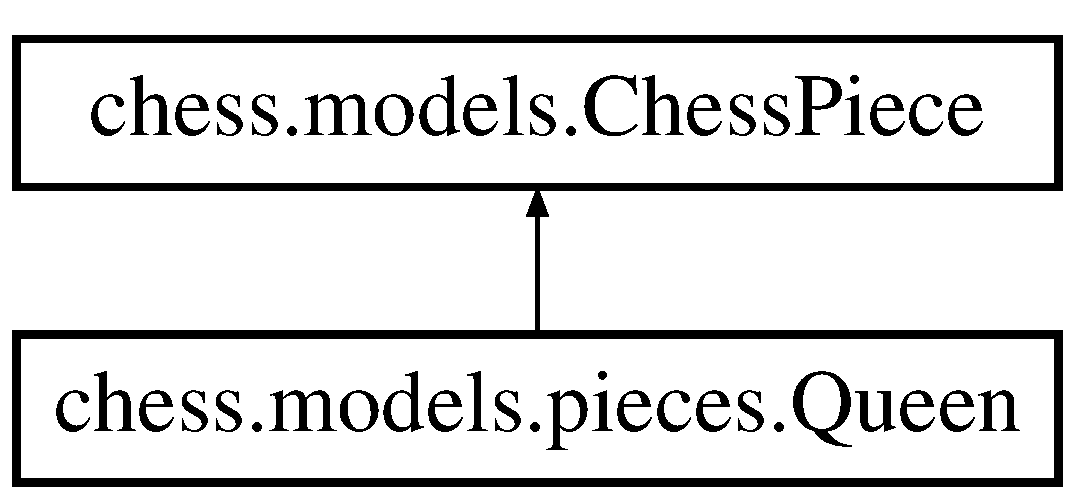
\includegraphics[height=2.000000cm]{classchess_1_1models_1_1pieces_1_1_queen}
\end{center}
\end{figure}
\subsection*{Public Member Functions}
\begin{DoxyCompactItemize}
\item 
\mbox{\hyperlink{classchess_1_1models_1_1pieces_1_1_queen_acc127213b82632b23448f334512b34b8}{Queen}} (\mbox{\hyperlink{enumchess_1_1models_1_1enums_1_1_player}{Player}} \mbox{\hyperlink{classchess_1_1models_1_1_chess_piece_a3bcc8a24667318b5aab8c146adcc3eb7}{player}}, \mbox{\hyperlink{classchess_1_1models_1_1_position}{Position}} \mbox{\hyperlink{classchess_1_1models_1_1_chess_piece_a0e4f8616b75e548f269d3971846396f3}{position}})
\item 
\mbox{\hyperlink{enumchess_1_1models_1_1enums_1_1_move_result}{Move\+Result}} \mbox{\hyperlink{classchess_1_1models_1_1pieces_1_1_queen_a99486b83609e973af4c09ddcf3582617}{is\+Legal\+Move}} (\mbox{\hyperlink{classchess_1_1models_1_1_position}{Position}} pos)
\item 
String \mbox{\hyperlink{classchess_1_1models_1_1pieces_1_1_queen_a723a09d8252bb14578d33c099242e37d}{to\+String}} ()
\end{DoxyCompactItemize}


\subsection{Detailed Description}
\mbox{\hyperlink{classchess_1_1models_1_1_chess_piece}{Chess\+Piece}} piece\+: \mbox{\hyperlink{classchess_1_1models_1_1pieces_1_1_queen}{Queen}} 

\subsection{Constructor \& Destructor Documentation}
\mbox{\Hypertarget{classchess_1_1models_1_1pieces_1_1_queen_acc127213b82632b23448f334512b34b8}\label{classchess_1_1models_1_1pieces_1_1_queen_acc127213b82632b23448f334512b34b8}} 
\index{chess\+::models\+::pieces\+::\+Queen@{chess\+::models\+::pieces\+::\+Queen}!Queen@{Queen}}
\index{Queen@{Queen}!chess\+::models\+::pieces\+::\+Queen@{chess\+::models\+::pieces\+::\+Queen}}
\subsubsection{\texorpdfstring{Queen()}{Queen()}}
{\footnotesize\ttfamily chess.\+models.\+pieces.\+Queen.\+Queen (\begin{DoxyParamCaption}\item[{\mbox{\hyperlink{enumchess_1_1models_1_1enums_1_1_player}{Player}}}]{player,  }\item[{\mbox{\hyperlink{classchess_1_1models_1_1_position}{Position}}}]{position }\end{DoxyParamCaption})}

Constructor of \mbox{\hyperlink{classchess_1_1models_1_1pieces_1_1_queen}{Queen}}


\begin{DoxyParams}{Parameters}
{\em player} & Belongs to which player \\
\hline
{\em position} & Initial position \\
\hline
\end{DoxyParams}


\subsection{Member Function Documentation}
\mbox{\Hypertarget{classchess_1_1models_1_1pieces_1_1_queen_a99486b83609e973af4c09ddcf3582617}\label{classchess_1_1models_1_1pieces_1_1_queen_a99486b83609e973af4c09ddcf3582617}} 
\index{chess\+::models\+::pieces\+::\+Queen@{chess\+::models\+::pieces\+::\+Queen}!is\+Legal\+Move@{is\+Legal\+Move}}
\index{is\+Legal\+Move@{is\+Legal\+Move}!chess\+::models\+::pieces\+::\+Queen@{chess\+::models\+::pieces\+::\+Queen}}
\subsubsection{\texorpdfstring{is\+Legal\+Move()}{isLegalMove()}}
{\footnotesize\ttfamily \mbox{\hyperlink{enumchess_1_1models_1_1enums_1_1_move_result}{Move\+Result}} chess.\+models.\+pieces.\+Queen.\+is\+Legal\+Move (\begin{DoxyParamCaption}\item[{\mbox{\hyperlink{classchess_1_1models_1_1_position}{Position}}}]{pos }\end{DoxyParamCaption})}

Check if the movement is legal


\begin{DoxyParams}{Parameters}
{\em pos} & Destination position \\
\hline
\end{DoxyParams}
\begin{DoxyReturn}{Returns}
Move\+Result 
\end{DoxyReturn}
\mbox{\Hypertarget{classchess_1_1models_1_1pieces_1_1_queen_a723a09d8252bb14578d33c099242e37d}\label{classchess_1_1models_1_1pieces_1_1_queen_a723a09d8252bb14578d33c099242e37d}} 
\index{chess\+::models\+::pieces\+::\+Queen@{chess\+::models\+::pieces\+::\+Queen}!to\+String@{to\+String}}
\index{to\+String@{to\+String}!chess\+::models\+::pieces\+::\+Queen@{chess\+::models\+::pieces\+::\+Queen}}
\subsubsection{\texorpdfstring{to\+String()}{toString()}}
{\footnotesize\ttfamily String chess.\+models.\+pieces.\+Queen.\+to\+String (\begin{DoxyParamCaption}{ }\end{DoxyParamCaption})}



The documentation for this class was generated from the following file\+:\begin{DoxyCompactItemize}
\item 
G\+:/\+Chess/src/main/java/chess/models/pieces/\mbox{\hyperlink{_queen_8java}{Queen.\+java}}\end{DoxyCompactItemize}

\hypertarget{classchess_1_1models_1_1pieces_1_1_queen_test}{}\section{chess.\+models.\+pieces.\+Queen\+Test Class Reference}
\label{classchess_1_1models_1_1pieces_1_1_queen_test}\index{chess.\+models.\+pieces.\+Queen\+Test@{chess.\+models.\+pieces.\+Queen\+Test}}
\subsection*{Public Member Functions}
\begin{DoxyCompactItemize}
\item 
void \mbox{\hyperlink{classchess_1_1models_1_1pieces_1_1_queen_test_a1881454d8fbe56b8c8f19895b048a81c}{is\+Legal\+Move}} ()
\end{DoxyCompactItemize}


\subsection{Member Function Documentation}
\mbox{\Hypertarget{classchess_1_1models_1_1pieces_1_1_queen_test_a1881454d8fbe56b8c8f19895b048a81c}\label{classchess_1_1models_1_1pieces_1_1_queen_test_a1881454d8fbe56b8c8f19895b048a81c}} 
\index{chess\+::models\+::pieces\+::\+Queen\+Test@{chess\+::models\+::pieces\+::\+Queen\+Test}!is\+Legal\+Move@{is\+Legal\+Move}}
\index{is\+Legal\+Move@{is\+Legal\+Move}!chess\+::models\+::pieces\+::\+Queen\+Test@{chess\+::models\+::pieces\+::\+Queen\+Test}}
\subsubsection{\texorpdfstring{is\+Legal\+Move()}{isLegalMove()}}
{\footnotesize\ttfamily void chess.\+models.\+pieces.\+Queen\+Test.\+is\+Legal\+Move (\begin{DoxyParamCaption}{ }\end{DoxyParamCaption})}



The documentation for this class was generated from the following file\+:\begin{DoxyCompactItemize}
\item 
G\+:/\+Chess/src/test/java/chess/models/pieces/\mbox{\hyperlink{_queen_test_8java}{Queen\+Test.\+java}}\end{DoxyCompactItemize}

\hypertarget{classchess_1_1command_1_1_request_chess_move}{}\section{chess.\+command.\+Request\+Chess\+Move Class Reference}
\label{classchess_1_1command_1_1_request_chess_move}\index{chess.\+command.\+Request\+Chess\+Move@{chess.\+command.\+Request\+Chess\+Move}}
\subsection*{Public Member Functions}
\begin{DoxyCompactItemize}
\item 
void \mbox{\hyperlink{classchess_1_1command_1_1_request_chess_move_a0c629dc3ed07c759b2345a713e836ad2}{set\+Move\+Command}} (\mbox{\hyperlink{interfacechess_1_1command_1_1_command}{Command}} command)
\item 
\mbox{\hyperlink{enumchess_1_1models_1_1enums_1_1_move_result}{Move\+Result}} \mbox{\hyperlink{classchess_1_1command_1_1_request_chess_move_ac8cda865cf4d3681717a37e0d74493a3}{execute\+Move\+Command}} (\mbox{\hyperlink{classchess_1_1models_1_1_board}{Board}} board, \mbox{\hyperlink{classchess_1_1models_1_1_chess_piece}{Chess\+Piece}} chess, \mbox{\hyperlink{classchess_1_1models_1_1_position}{Position}} destination)
\item 
List$<$ \mbox{\hyperlink{classchess_1_1models_1_1_position}{Position}} $>$ \mbox{\hyperlink{classchess_1_1command_1_1_request_chess_move_a24e98a1984e9e806b6e96c35ba11b40a}{undo\+Move\+Command}} (\mbox{\hyperlink{classchess_1_1models_1_1_board}{Board}} board)
\end{DoxyCompactItemize}


\subsection{Detailed Description}
Invoker of the \mbox{\hyperlink{interfacechess_1_1command_1_1_command}{Command}} Pattern 

\subsection{Member Function Documentation}
\mbox{\Hypertarget{classchess_1_1command_1_1_request_chess_move_ac8cda865cf4d3681717a37e0d74493a3}\label{classchess_1_1command_1_1_request_chess_move_ac8cda865cf4d3681717a37e0d74493a3}} 
\index{chess\+::command\+::\+Request\+Chess\+Move@{chess\+::command\+::\+Request\+Chess\+Move}!execute\+Move\+Command@{execute\+Move\+Command}}
\index{execute\+Move\+Command@{execute\+Move\+Command}!chess\+::command\+::\+Request\+Chess\+Move@{chess\+::command\+::\+Request\+Chess\+Move}}
\subsubsection{\texorpdfstring{execute\+Move\+Command()}{executeMoveCommand()}}
{\footnotesize\ttfamily \mbox{\hyperlink{enumchess_1_1models_1_1enums_1_1_move_result}{Move\+Result}} chess.\+command.\+Request\+Chess\+Move.\+execute\+Move\+Command (\begin{DoxyParamCaption}\item[{\mbox{\hyperlink{classchess_1_1models_1_1_board}{Board}}}]{board,  }\item[{\mbox{\hyperlink{classchess_1_1models_1_1_chess_piece}{Chess\+Piece}}}]{chess,  }\item[{\mbox{\hyperlink{classchess_1_1models_1_1_position}{Position}}}]{destination }\end{DoxyParamCaption})}

Execute command


\begin{DoxyParams}{Parameters}
{\em board} & Chess board \\
\hline
{\em chess} & Piece that needs to move \\
\hline
{\em destination} & Destination position \\
\hline
\end{DoxyParams}
\mbox{\Hypertarget{classchess_1_1command_1_1_request_chess_move_a0c629dc3ed07c759b2345a713e836ad2}\label{classchess_1_1command_1_1_request_chess_move_a0c629dc3ed07c759b2345a713e836ad2}} 
\index{chess\+::command\+::\+Request\+Chess\+Move@{chess\+::command\+::\+Request\+Chess\+Move}!set\+Move\+Command@{set\+Move\+Command}}
\index{set\+Move\+Command@{set\+Move\+Command}!chess\+::command\+::\+Request\+Chess\+Move@{chess\+::command\+::\+Request\+Chess\+Move}}
\subsubsection{\texorpdfstring{set\+Move\+Command()}{setMoveCommand()}}
{\footnotesize\ttfamily void chess.\+command.\+Request\+Chess\+Move.\+set\+Move\+Command (\begin{DoxyParamCaption}\item[{\mbox{\hyperlink{interfacechess_1_1command_1_1_command}{Command}}}]{command }\end{DoxyParamCaption})}

Set command


\begin{DoxyParams}{Parameters}
{\em command} & Chess move command \\
\hline
\end{DoxyParams}
\mbox{\Hypertarget{classchess_1_1command_1_1_request_chess_move_a24e98a1984e9e806b6e96c35ba11b40a}\label{classchess_1_1command_1_1_request_chess_move_a24e98a1984e9e806b6e96c35ba11b40a}} 
\index{chess\+::command\+::\+Request\+Chess\+Move@{chess\+::command\+::\+Request\+Chess\+Move}!undo\+Move\+Command@{undo\+Move\+Command}}
\index{undo\+Move\+Command@{undo\+Move\+Command}!chess\+::command\+::\+Request\+Chess\+Move@{chess\+::command\+::\+Request\+Chess\+Move}}
\subsubsection{\texorpdfstring{undo\+Move\+Command()}{undoMoveCommand()}}
{\footnotesize\ttfamily List$<$\mbox{\hyperlink{classchess_1_1models_1_1_position}{Position}}$>$ chess.\+command.\+Request\+Chess\+Move.\+undo\+Move\+Command (\begin{DoxyParamCaption}\item[{\mbox{\hyperlink{classchess_1_1models_1_1_board}{Board}}}]{board }\end{DoxyParamCaption})}

Undo command


\begin{DoxyParams}{Parameters}
{\em board} & Chess board \\
\hline
\end{DoxyParams}
\begin{DoxyReturn}{Returns}
The chess\textquotesingle{}s positions before undo and after undo 
\end{DoxyReturn}


The documentation for this class was generated from the following file\+:\begin{DoxyCompactItemize}
\item 
src/main/java/chess/command/\mbox{\hyperlink{_request_chess_move_8java}{Request\+Chess\+Move.\+java}}\end{DoxyCompactItemize}

\hypertarget{classchess_1_1models_1_1pieces_1_1_rook}{}\section{chess.\+models.\+pieces.\+Rook Class Reference}
\label{classchess_1_1models_1_1pieces_1_1_rook}\index{chess.\+models.\+pieces.\+Rook@{chess.\+models.\+pieces.\+Rook}}
Inheritance diagram for chess.\+models.\+pieces.\+Rook\+:\begin{figure}[H]
\begin{center}
\leavevmode
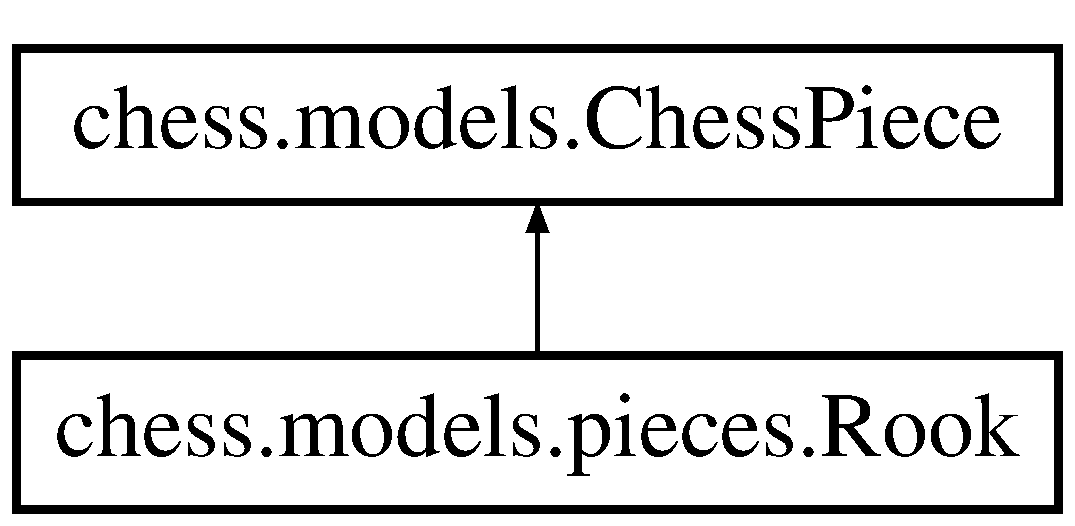
\includegraphics[height=2.000000cm]{classchess_1_1models_1_1pieces_1_1_rook}
\end{center}
\end{figure}
\subsection*{Public Member Functions}
\begin{DoxyCompactItemize}
\item 
\mbox{\hyperlink{classchess_1_1models_1_1pieces_1_1_rook_a6a09ddec79bb71f7b497e0faf8b02152}{Rook}} (\mbox{\hyperlink{enumchess_1_1models_1_1enums_1_1_player}{Player}} player, \mbox{\hyperlink{classchess_1_1models_1_1_position}{Position}} position)
\item 
\mbox{\hyperlink{enumchess_1_1models_1_1enums_1_1_move_result}{Move\+Result}} \mbox{\hyperlink{classchess_1_1models_1_1pieces_1_1_rook_adf20fa1c361d9122cae9fd20f543f8e4}{is\+Legal\+Move}} (\mbox{\hyperlink{classchess_1_1models_1_1_position}{Position}} pos)
\item 
String \mbox{\hyperlink{classchess_1_1models_1_1pieces_1_1_rook_a73f28ce35486a866fabe250ad4490993}{to\+String}} ()
\end{DoxyCompactItemize}


\subsection{Detailed Description}
\mbox{\hyperlink{classchess_1_1models_1_1_chess_piece}{Chess\+Piece}} piece\+: \mbox{\hyperlink{classchess_1_1models_1_1pieces_1_1_rook}{Rook}} 

\subsection{Constructor \& Destructor Documentation}
\mbox{\Hypertarget{classchess_1_1models_1_1pieces_1_1_rook_a6a09ddec79bb71f7b497e0faf8b02152}\label{classchess_1_1models_1_1pieces_1_1_rook_a6a09ddec79bb71f7b497e0faf8b02152}} 
\index{chess\+::models\+::pieces\+::\+Rook@{chess\+::models\+::pieces\+::\+Rook}!Rook@{Rook}}
\index{Rook@{Rook}!chess\+::models\+::pieces\+::\+Rook@{chess\+::models\+::pieces\+::\+Rook}}
\subsubsection{\texorpdfstring{Rook()}{Rook()}}
{\footnotesize\ttfamily chess.\+models.\+pieces.\+Rook.\+Rook (\begin{DoxyParamCaption}\item[{\mbox{\hyperlink{enumchess_1_1models_1_1enums_1_1_player}{Player}}}]{player,  }\item[{\mbox{\hyperlink{classchess_1_1models_1_1_position}{Position}}}]{position }\end{DoxyParamCaption})}

Constructor of \mbox{\hyperlink{classchess_1_1models_1_1pieces_1_1_rook}{Rook}}


\begin{DoxyParams}{Parameters}
{\em player} & Belongs to which player \\
\hline
{\em position} & Initial position \\
\hline
\end{DoxyParams}


\subsection{Member Function Documentation}
\mbox{\Hypertarget{classchess_1_1models_1_1pieces_1_1_rook_adf20fa1c361d9122cae9fd20f543f8e4}\label{classchess_1_1models_1_1pieces_1_1_rook_adf20fa1c361d9122cae9fd20f543f8e4}} 
\index{chess\+::models\+::pieces\+::\+Rook@{chess\+::models\+::pieces\+::\+Rook}!is\+Legal\+Move@{is\+Legal\+Move}}
\index{is\+Legal\+Move@{is\+Legal\+Move}!chess\+::models\+::pieces\+::\+Rook@{chess\+::models\+::pieces\+::\+Rook}}
\subsubsection{\texorpdfstring{is\+Legal\+Move()}{isLegalMove()}}
{\footnotesize\ttfamily \mbox{\hyperlink{enumchess_1_1models_1_1enums_1_1_move_result}{Move\+Result}} chess.\+models.\+pieces.\+Rook.\+is\+Legal\+Move (\begin{DoxyParamCaption}\item[{\mbox{\hyperlink{classchess_1_1models_1_1_position}{Position}}}]{pos }\end{DoxyParamCaption})}

Check if the movement is legal


\begin{DoxyParams}{Parameters}
{\em pos} & Destination position \\
\hline
\end{DoxyParams}
\begin{DoxyReturn}{Returns}
Move\+Result 
\end{DoxyReturn}
\mbox{\Hypertarget{classchess_1_1models_1_1pieces_1_1_rook_a73f28ce35486a866fabe250ad4490993}\label{classchess_1_1models_1_1pieces_1_1_rook_a73f28ce35486a866fabe250ad4490993}} 
\index{chess\+::models\+::pieces\+::\+Rook@{chess\+::models\+::pieces\+::\+Rook}!to\+String@{to\+String}}
\index{to\+String@{to\+String}!chess\+::models\+::pieces\+::\+Rook@{chess\+::models\+::pieces\+::\+Rook}}
\subsubsection{\texorpdfstring{to\+String()}{toString()}}
{\footnotesize\ttfamily String chess.\+models.\+pieces.\+Rook.\+to\+String (\begin{DoxyParamCaption}{ }\end{DoxyParamCaption})}



The documentation for this class was generated from the following file\+:\begin{DoxyCompactItemize}
\item 
src/main/java/chess/models/pieces/\mbox{\hyperlink{_rook_8java}{Rook.\+java}}\end{DoxyCompactItemize}

\hypertarget{classchess_1_1models_1_1pieces_1_1_rook_test}{}\section{chess.\+models.\+pieces.\+Rook\+Test Class Reference}
\label{classchess_1_1models_1_1pieces_1_1_rook_test}\index{chess.\+models.\+pieces.\+Rook\+Test@{chess.\+models.\+pieces.\+Rook\+Test}}
\subsection*{Public Member Functions}
\begin{DoxyCompactItemize}
\item 
void \mbox{\hyperlink{classchess_1_1models_1_1pieces_1_1_rook_test_a3c56b66f7159677ac04305b4029c58ca}{is\+Legal\+Move}} ()
\end{DoxyCompactItemize}


\subsection{Member Function Documentation}
\mbox{\Hypertarget{classchess_1_1models_1_1pieces_1_1_rook_test_a3c56b66f7159677ac04305b4029c58ca}\label{classchess_1_1models_1_1pieces_1_1_rook_test_a3c56b66f7159677ac04305b4029c58ca}} 
\index{chess\+::models\+::pieces\+::\+Rook\+Test@{chess\+::models\+::pieces\+::\+Rook\+Test}!is\+Legal\+Move@{is\+Legal\+Move}}
\index{is\+Legal\+Move@{is\+Legal\+Move}!chess\+::models\+::pieces\+::\+Rook\+Test@{chess\+::models\+::pieces\+::\+Rook\+Test}}
\subsubsection{\texorpdfstring{is\+Legal\+Move()}{isLegalMove()}}
{\footnotesize\ttfamily void chess.\+models.\+pieces.\+Rook\+Test.\+is\+Legal\+Move (\begin{DoxyParamCaption}{ }\end{DoxyParamCaption})}



The documentation for this class was generated from the following file\+:\begin{DoxyCompactItemize}
\item 
src/test/java/chess/models/pieces/\mbox{\hyperlink{_rook_test_8java}{Rook\+Test.\+java}}\end{DoxyCompactItemize}

\hypertarget{classchess_1_1models_1_1pieces_1_1_soldier}{}\section{chess.\+models.\+pieces.\+Soldier Class Reference}
\label{classchess_1_1models_1_1pieces_1_1_soldier}\index{chess.\+models.\+pieces.\+Soldier@{chess.\+models.\+pieces.\+Soldier}}
Inheritance diagram for chess.\+models.\+pieces.\+Soldier\+:\begin{figure}[H]
\begin{center}
\leavevmode
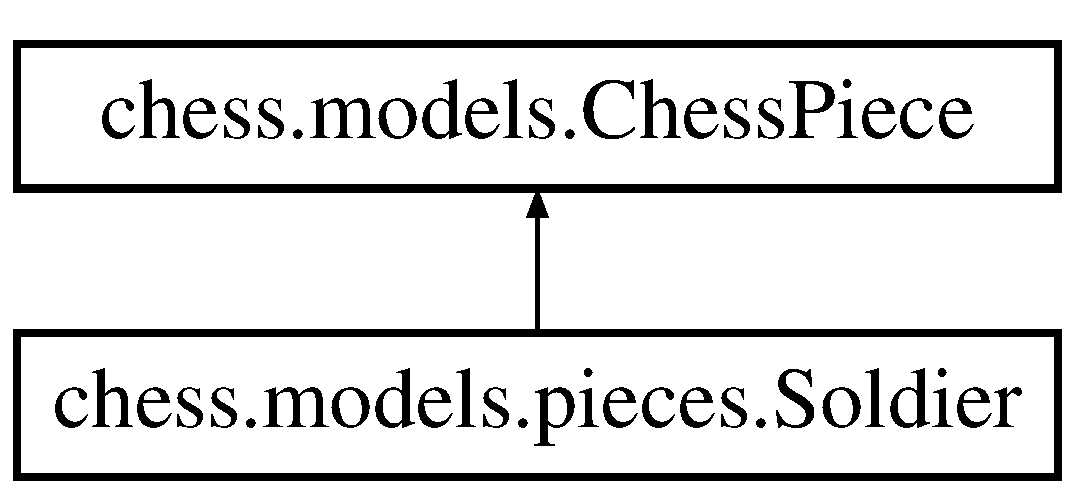
\includegraphics[height=2.000000cm]{classchess_1_1models_1_1pieces_1_1_soldier}
\end{center}
\end{figure}
\subsection*{Public Member Functions}
\begin{DoxyCompactItemize}
\item 
\mbox{\hyperlink{classchess_1_1models_1_1pieces_1_1_soldier_a3de8743b5a054a97b126297e3e5fea36}{Soldier}} (\mbox{\hyperlink{enumchess_1_1models_1_1enums_1_1_player}{Player}} player, \mbox{\hyperlink{classchess_1_1models_1_1_position}{Position}} position)
\item 
\mbox{\hyperlink{enumchess_1_1models_1_1enums_1_1_move_result}{Move\+Result}} \mbox{\hyperlink{classchess_1_1models_1_1pieces_1_1_soldier_a5a0cc5ebe1f0a4b2b68b9359f5bad0c5}{is\+Legal\+Move}} (\mbox{\hyperlink{classchess_1_1models_1_1_position}{Position}} pos)
\item 
boolean \mbox{\hyperlink{classchess_1_1models_1_1pieces_1_1_soldier_a3be305544d8e788663b6c394d334f596}{is\+Forward}} (\mbox{\hyperlink{classchess_1_1models_1_1_position}{Position}} pos)
\item 
boolean \mbox{\hyperlink{classchess_1_1models_1_1pieces_1_1_soldier_a9ee2ecb79068bd41f01608f23cd8dd01}{is\+Cross\+The\+River}} ()
\end{DoxyCompactItemize}


\subsection{Detailed Description}
Custom chess piece\+: \mbox{\hyperlink{classchess_1_1models_1_1pieces_1_1_soldier}{Soldier}} \mbox{\hyperlink{classchess_1_1models_1_1pieces_1_1_soldier}{Soldier}} is Chinese \mbox{\hyperlink{classchess_1_1models_1_1pieces_1_1_pawn}{Pawn}}. It move and capture by advancing one point before it crossed the river(the half of ths board). Once they have crossed the river, they may also move and capture one point horizontally. 

\subsection{Constructor \& Destructor Documentation}
\mbox{\Hypertarget{classchess_1_1models_1_1pieces_1_1_soldier_a3de8743b5a054a97b126297e3e5fea36}\label{classchess_1_1models_1_1pieces_1_1_soldier_a3de8743b5a054a97b126297e3e5fea36}} 
\index{chess\+::models\+::pieces\+::\+Soldier@{chess\+::models\+::pieces\+::\+Soldier}!Soldier@{Soldier}}
\index{Soldier@{Soldier}!chess\+::models\+::pieces\+::\+Soldier@{chess\+::models\+::pieces\+::\+Soldier}}
\subsubsection{\texorpdfstring{Soldier()}{Soldier()}}
{\footnotesize\ttfamily chess.\+models.\+pieces.\+Soldier.\+Soldier (\begin{DoxyParamCaption}\item[{\mbox{\hyperlink{enumchess_1_1models_1_1enums_1_1_player}{Player}}}]{player,  }\item[{\mbox{\hyperlink{classchess_1_1models_1_1_position}{Position}}}]{position }\end{DoxyParamCaption})}

Constructor of \mbox{\hyperlink{classchess_1_1models_1_1pieces_1_1_soldier}{Soldier}}


\begin{DoxyParams}{Parameters}
{\em player} & Belongs to which player \\
\hline
{\em position} & Initial position \\
\hline
\end{DoxyParams}


\subsection{Member Function Documentation}
\mbox{\Hypertarget{classchess_1_1models_1_1pieces_1_1_soldier_a9ee2ecb79068bd41f01608f23cd8dd01}\label{classchess_1_1models_1_1pieces_1_1_soldier_a9ee2ecb79068bd41f01608f23cd8dd01}} 
\index{chess\+::models\+::pieces\+::\+Soldier@{chess\+::models\+::pieces\+::\+Soldier}!is\+Cross\+The\+River@{is\+Cross\+The\+River}}
\index{is\+Cross\+The\+River@{is\+Cross\+The\+River}!chess\+::models\+::pieces\+::\+Soldier@{chess\+::models\+::pieces\+::\+Soldier}}
\subsubsection{\texorpdfstring{is\+Cross\+The\+River()}{isCrossTheRiver()}}
{\footnotesize\ttfamily boolean chess.\+models.\+pieces.\+Soldier.\+is\+Cross\+The\+River (\begin{DoxyParamCaption}{ }\end{DoxyParamCaption})}

Check if the soldier cross the river

\begin{DoxyReturn}{Returns}
true is that the soldier have crossed the river 
\end{DoxyReturn}
\mbox{\Hypertarget{classchess_1_1models_1_1pieces_1_1_soldier_a3be305544d8e788663b6c394d334f596}\label{classchess_1_1models_1_1pieces_1_1_soldier_a3be305544d8e788663b6c394d334f596}} 
\index{chess\+::models\+::pieces\+::\+Soldier@{chess\+::models\+::pieces\+::\+Soldier}!is\+Forward@{is\+Forward}}
\index{is\+Forward@{is\+Forward}!chess\+::models\+::pieces\+::\+Soldier@{chess\+::models\+::pieces\+::\+Soldier}}
\subsubsection{\texorpdfstring{is\+Forward()}{isForward()}}
{\footnotesize\ttfamily boolean chess.\+models.\+pieces.\+Soldier.\+is\+Forward (\begin{DoxyParamCaption}\item[{\mbox{\hyperlink{classchess_1_1models_1_1_position}{Position}}}]{pos }\end{DoxyParamCaption})}

Check if the soldier is moving forward


\begin{DoxyParams}{Parameters}
{\em pos} & Destination position \\
\hline
\end{DoxyParams}
\begin{DoxyReturn}{Returns}
true is that the soldier is moving forward 
\end{DoxyReturn}
\mbox{\Hypertarget{classchess_1_1models_1_1pieces_1_1_soldier_a5a0cc5ebe1f0a4b2b68b9359f5bad0c5}\label{classchess_1_1models_1_1pieces_1_1_soldier_a5a0cc5ebe1f0a4b2b68b9359f5bad0c5}} 
\index{chess\+::models\+::pieces\+::\+Soldier@{chess\+::models\+::pieces\+::\+Soldier}!is\+Legal\+Move@{is\+Legal\+Move}}
\index{is\+Legal\+Move@{is\+Legal\+Move}!chess\+::models\+::pieces\+::\+Soldier@{chess\+::models\+::pieces\+::\+Soldier}}
\subsubsection{\texorpdfstring{is\+Legal\+Move()}{isLegalMove()}}
{\footnotesize\ttfamily \mbox{\hyperlink{enumchess_1_1models_1_1enums_1_1_move_result}{Move\+Result}} chess.\+models.\+pieces.\+Soldier.\+is\+Legal\+Move (\begin{DoxyParamCaption}\item[{\mbox{\hyperlink{classchess_1_1models_1_1_position}{Position}}}]{pos }\end{DoxyParamCaption})}

Check if the movement is legal


\begin{DoxyParams}{Parameters}
{\em pos} & Destination position \\
\hline
\end{DoxyParams}
\begin{DoxyReturn}{Returns}
Move\+Result 
\end{DoxyReturn}


The documentation for this class was generated from the following file\+:\begin{DoxyCompactItemize}
\item 
src/main/java/chess/models/pieces/\mbox{\hyperlink{_soldier_8java}{Soldier.\+java}}\end{DoxyCompactItemize}

\hypertarget{classchess_1_1models_1_1pieces_1_1_soldier_test}{}\section{chess.\+models.\+pieces.\+Soldier\+Test Class Reference}
\label{classchess_1_1models_1_1pieces_1_1_soldier_test}\index{chess.\+models.\+pieces.\+Soldier\+Test@{chess.\+models.\+pieces.\+Soldier\+Test}}
\subsection*{Public Member Functions}
\begin{DoxyCompactItemize}
\item 
void \mbox{\hyperlink{classchess_1_1models_1_1pieces_1_1_soldier_test_ad6deec316336baea729d2c952597cbf7}{is\+Legal\+Move}} ()
\item 
void \mbox{\hyperlink{classchess_1_1models_1_1pieces_1_1_soldier_test_a69e114cbe42f94b7d3d2f5621bdbcd3b}{is\+Forward}} ()
\item 
void \mbox{\hyperlink{classchess_1_1models_1_1pieces_1_1_soldier_test_a3c0c320ad093d44527016c587362d0db}{is\+Cross\+The\+River}} ()
\end{DoxyCompactItemize}


\subsection{Member Function Documentation}
\mbox{\Hypertarget{classchess_1_1models_1_1pieces_1_1_soldier_test_a3c0c320ad093d44527016c587362d0db}\label{classchess_1_1models_1_1pieces_1_1_soldier_test_a3c0c320ad093d44527016c587362d0db}} 
\index{chess\+::models\+::pieces\+::\+Soldier\+Test@{chess\+::models\+::pieces\+::\+Soldier\+Test}!is\+Cross\+The\+River@{is\+Cross\+The\+River}}
\index{is\+Cross\+The\+River@{is\+Cross\+The\+River}!chess\+::models\+::pieces\+::\+Soldier\+Test@{chess\+::models\+::pieces\+::\+Soldier\+Test}}
\subsubsection{\texorpdfstring{is\+Cross\+The\+River()}{isCrossTheRiver()}}
{\footnotesize\ttfamily void chess.\+models.\+pieces.\+Soldier\+Test.\+is\+Cross\+The\+River (\begin{DoxyParamCaption}{ }\end{DoxyParamCaption})}

Method\+: \mbox{\hyperlink{classchess_1_1models_1_1pieces_1_1_soldier_test_a3c0c320ad093d44527016c587362d0db}{is\+Cross\+The\+River()}} \mbox{\Hypertarget{classchess_1_1models_1_1pieces_1_1_soldier_test_a69e114cbe42f94b7d3d2f5621bdbcd3b}\label{classchess_1_1models_1_1pieces_1_1_soldier_test_a69e114cbe42f94b7d3d2f5621bdbcd3b}} 
\index{chess\+::models\+::pieces\+::\+Soldier\+Test@{chess\+::models\+::pieces\+::\+Soldier\+Test}!is\+Forward@{is\+Forward}}
\index{is\+Forward@{is\+Forward}!chess\+::models\+::pieces\+::\+Soldier\+Test@{chess\+::models\+::pieces\+::\+Soldier\+Test}}
\subsubsection{\texorpdfstring{is\+Forward()}{isForward()}}
{\footnotesize\ttfamily void chess.\+models.\+pieces.\+Soldier\+Test.\+is\+Forward (\begin{DoxyParamCaption}{ }\end{DoxyParamCaption})}

Method\+: is\+Forward(\+Position pos) \mbox{\Hypertarget{classchess_1_1models_1_1pieces_1_1_soldier_test_ad6deec316336baea729d2c952597cbf7}\label{classchess_1_1models_1_1pieces_1_1_soldier_test_ad6deec316336baea729d2c952597cbf7}} 
\index{chess\+::models\+::pieces\+::\+Soldier\+Test@{chess\+::models\+::pieces\+::\+Soldier\+Test}!is\+Legal\+Move@{is\+Legal\+Move}}
\index{is\+Legal\+Move@{is\+Legal\+Move}!chess\+::models\+::pieces\+::\+Soldier\+Test@{chess\+::models\+::pieces\+::\+Soldier\+Test}}
\subsubsection{\texorpdfstring{is\+Legal\+Move()}{isLegalMove()}}
{\footnotesize\ttfamily void chess.\+models.\+pieces.\+Soldier\+Test.\+is\+Legal\+Move (\begin{DoxyParamCaption}{ }\end{DoxyParamCaption})}

Method\+: is\+Legal\+Move(\+Position pos) 

The documentation for this class was generated from the following file\+:\begin{DoxyCompactItemize}
\item 
G\+:/\+Chess/src/test/java/chess/models/pieces/\mbox{\hyperlink{_soldier_test_8java}{Soldier\+Test.\+java}}\end{DoxyCompactItemize}

\chapter{File Documentation}
\hypertarget{_chess_move_8java}{}\section{src/main/java/chess/command/\+Chess\+Move.java File Reference}
\label{_chess_move_8java}\index{src/main/java/chess/command/\+Chess\+Move.\+java@{src/main/java/chess/command/\+Chess\+Move.\+java}}
\subsection*{Classes}
\begin{DoxyCompactItemize}
\item 
class \mbox{\hyperlink{classchess_1_1command_1_1_chess_move}{chess.\+command.\+Chess\+Move}}
\end{DoxyCompactItemize}
\subsection*{Packages}
\begin{DoxyCompactItemize}
\item 
package \mbox{\hyperlink{namespacechess_1_1command}{chess.\+command}}
\end{DoxyCompactItemize}

\hypertarget{_chess_move_command_8java}{}\section{src/main/java/chess/command/\+Chess\+Move\+Command.java File Reference}
\label{_chess_move_command_8java}\index{src/main/java/chess/command/\+Chess\+Move\+Command.\+java@{src/main/java/chess/command/\+Chess\+Move\+Command.\+java}}
\subsection*{Classes}
\begin{DoxyCompactItemize}
\item 
class \mbox{\hyperlink{classchess_1_1command_1_1_chess_move_command}{chess.\+command.\+Chess\+Move\+Command}}
\end{DoxyCompactItemize}
\subsection*{Packages}
\begin{DoxyCompactItemize}
\item 
package \mbox{\hyperlink{namespacechess_1_1command}{chess.\+command}}
\end{DoxyCompactItemize}

\hypertarget{_command_8java}{}\section{src/main/java/chess/command/\+Command.java File Reference}
\label{_command_8java}\index{src/main/java/chess/command/\+Command.\+java@{src/main/java/chess/command/\+Command.\+java}}
\subsection*{Classes}
\begin{DoxyCompactItemize}
\item 
interface \mbox{\hyperlink{interfacechess_1_1command_1_1_command}{chess.\+command.\+Command}}
\end{DoxyCompactItemize}
\subsection*{Packages}
\begin{DoxyCompactItemize}
\item 
package \mbox{\hyperlink{namespacechess_1_1command}{chess.\+command}}
\end{DoxyCompactItemize}

\hypertarget{_request_chess_move_8java}{}\section{src/main/java/chess/command/\+Request\+Chess\+Move.java File Reference}
\label{_request_chess_move_8java}\index{src/main/java/chess/command/\+Request\+Chess\+Move.\+java@{src/main/java/chess/command/\+Request\+Chess\+Move.\+java}}
\subsection*{Classes}
\begin{DoxyCompactItemize}
\item 
class \mbox{\hyperlink{classchess_1_1command_1_1_request_chess_move}{chess.\+command.\+Request\+Chess\+Move}}
\end{DoxyCompactItemize}
\subsection*{Packages}
\begin{DoxyCompactItemize}
\item 
package \mbox{\hyperlink{namespacechess_1_1command}{chess.\+command}}
\end{DoxyCompactItemize}

\hypertarget{_board_controller_8java}{}\section{G\+:/\+Chess/src/main/java/chess/controllers/\+Board\+Controller.java File Reference}
\label{_board_controller_8java}\index{G\+:/\+Chess/src/main/java/chess/controllers/\+Board\+Controller.\+java@{G\+:/\+Chess/src/main/java/chess/controllers/\+Board\+Controller.\+java}}
\subsection*{Classes}
\begin{DoxyCompactItemize}
\item 
class \mbox{\hyperlink{classchess_1_1controllers_1_1_board_controller}{chess.\+controllers.\+Board\+Controller}}
\end{DoxyCompactItemize}
\subsection*{Packages}
\begin{DoxyCompactItemize}
\item 
package \mbox{\hyperlink{namespacechess_1_1controllers}{chess.\+controllers}}
\end{DoxyCompactItemize}

\hypertarget{_main_8java}{}\section{src/main/java/chess/main/\+Main.java File Reference}
\label{_main_8java}\index{src/main/java/chess/main/\+Main.\+java@{src/main/java/chess/main/\+Main.\+java}}
\subsection*{Classes}
\begin{DoxyCompactItemize}
\item 
class \mbox{\hyperlink{classchess_1_1main_1_1_main}{chess.\+main.\+Main}}
\end{DoxyCompactItemize}
\subsection*{Packages}
\begin{DoxyCompactItemize}
\item 
package \mbox{\hyperlink{namespacechess_1_1main}{chess.\+main}}
\end{DoxyCompactItemize}

\hypertarget{_board_8java}{}\section{G\+:/\+Chess/src/main/java/chess/models/\+Board.java File Reference}
\label{_board_8java}\index{G\+:/\+Chess/src/main/java/chess/models/\+Board.\+java@{G\+:/\+Chess/src/main/java/chess/models/\+Board.\+java}}
\subsection*{Classes}
\begin{DoxyCompactItemize}
\item 
class \mbox{\hyperlink{classchess_1_1models_1_1_board}{chess.\+models.\+Board}}
\end{DoxyCompactItemize}
\subsection*{Packages}
\begin{DoxyCompactItemize}
\item 
package \mbox{\hyperlink{namespacechess_1_1models}{chess.\+models}}
\end{DoxyCompactItemize}

\hypertarget{_chess_piece_8java}{}\section{src/main/java/chess/models/\+Chess\+Piece.java File Reference}
\label{_chess_piece_8java}\index{src/main/java/chess/models/\+Chess\+Piece.\+java@{src/main/java/chess/models/\+Chess\+Piece.\+java}}
\subsection*{Classes}
\begin{DoxyCompactItemize}
\item 
class \mbox{\hyperlink{classchess_1_1models_1_1_chess_piece}{chess.\+models.\+Chess\+Piece}}
\end{DoxyCompactItemize}
\subsection*{Packages}
\begin{DoxyCompactItemize}
\item 
package \mbox{\hyperlink{namespacechess_1_1models}{chess.\+models}}
\end{DoxyCompactItemize}

\hypertarget{_game_mode_8java}{}\section{src/main/java/chess/models/enums/\+Game\+Mode.java File Reference}
\label{_game_mode_8java}\index{src/main/java/chess/models/enums/\+Game\+Mode.\+java@{src/main/java/chess/models/enums/\+Game\+Mode.\+java}}
\subsection*{Classes}
\begin{DoxyCompactItemize}
\item 
enum \mbox{\hyperlink{enumchess_1_1models_1_1enums_1_1_game_mode}{chess.\+models.\+enums.\+Game\+Mode}}
\end{DoxyCompactItemize}
\subsection*{Packages}
\begin{DoxyCompactItemize}
\item 
package \mbox{\hyperlink{namespacechess_1_1models_1_1enums}{chess.\+models.\+enums}}
\end{DoxyCompactItemize}

\hypertarget{_game_result_8java}{}\section{src/main/java/chess/models/enums/\+Game\+Result.java File Reference}
\label{_game_result_8java}\index{src/main/java/chess/models/enums/\+Game\+Result.\+java@{src/main/java/chess/models/enums/\+Game\+Result.\+java}}
\subsection*{Classes}
\begin{DoxyCompactItemize}
\item 
enum \mbox{\hyperlink{enumchess_1_1models_1_1enums_1_1_game_result}{chess.\+models.\+enums.\+Game\+Result}}
\end{DoxyCompactItemize}
\subsection*{Packages}
\begin{DoxyCompactItemize}
\item 
package \mbox{\hyperlink{namespacechess_1_1models_1_1enums}{chess.\+models.\+enums}}
\end{DoxyCompactItemize}

\hypertarget{_move_result_8java}{}\section{src/main/java/chess/models/enums/\+Move\+Result.java File Reference}
\label{_move_result_8java}\index{src/main/java/chess/models/enums/\+Move\+Result.\+java@{src/main/java/chess/models/enums/\+Move\+Result.\+java}}
\subsection*{Classes}
\begin{DoxyCompactItemize}
\item 
enum \mbox{\hyperlink{enumchess_1_1models_1_1enums_1_1_move_result}{chess.\+models.\+enums.\+Move\+Result}}
\end{DoxyCompactItemize}
\subsection*{Packages}
\begin{DoxyCompactItemize}
\item 
package \mbox{\hyperlink{namespacechess_1_1models_1_1enums}{chess.\+models.\+enums}}
\end{DoxyCompactItemize}

\hypertarget{_player_8java}{}\section{src/main/java/chess/models/enums/\+Player.java File Reference}
\label{_player_8java}\index{src/main/java/chess/models/enums/\+Player.\+java@{src/main/java/chess/models/enums/\+Player.\+java}}
\subsection*{Classes}
\begin{DoxyCompactItemize}
\item 
enum \mbox{\hyperlink{enumchess_1_1models_1_1enums_1_1_player}{chess.\+models.\+enums.\+Player}}
\end{DoxyCompactItemize}
\subsection*{Packages}
\begin{DoxyCompactItemize}
\item 
package \mbox{\hyperlink{namespacechess_1_1models_1_1enums}{chess.\+models.\+enums}}
\end{DoxyCompactItemize}

\hypertarget{_path_8java}{}\section{G\+:/\+Chess/src/main/java/chess/models/\+Path.java File Reference}
\label{_path_8java}\index{G\+:/\+Chess/src/main/java/chess/models/\+Path.\+java@{G\+:/\+Chess/src/main/java/chess/models/\+Path.\+java}}
\subsection*{Classes}
\begin{DoxyCompactItemize}
\item 
class \mbox{\hyperlink{classchess_1_1models_1_1_path}{chess.\+models.\+Path}}
\end{DoxyCompactItemize}
\subsection*{Packages}
\begin{DoxyCompactItemize}
\item 
package \mbox{\hyperlink{namespacechess_1_1models}{chess.\+models}}
\end{DoxyCompactItemize}

\hypertarget{_advisor_8java}{}\section{G\+:/\+Chess/src/main/java/chess/models/pieces/\+Advisor.java File Reference}
\label{_advisor_8java}\index{G\+:/\+Chess/src/main/java/chess/models/pieces/\+Advisor.\+java@{G\+:/\+Chess/src/main/java/chess/models/pieces/\+Advisor.\+java}}
\subsection*{Classes}
\begin{DoxyCompactItemize}
\item 
class \mbox{\hyperlink{classchess_1_1models_1_1pieces_1_1_advisor}{chess.\+models.\+pieces.\+Advisor}}
\end{DoxyCompactItemize}
\subsection*{Packages}
\begin{DoxyCompactItemize}
\item 
package \mbox{\hyperlink{namespacechess_1_1models_1_1pieces}{chess.\+models.\+pieces}}
\end{DoxyCompactItemize}

\hypertarget{_bishop_8java}{}\section{G\+:/\+Chess/src/main/java/chess/models/pieces/\+Bishop.java File Reference}
\label{_bishop_8java}\index{G\+:/\+Chess/src/main/java/chess/models/pieces/\+Bishop.\+java@{G\+:/\+Chess/src/main/java/chess/models/pieces/\+Bishop.\+java}}
\subsection*{Classes}
\begin{DoxyCompactItemize}
\item 
class \mbox{\hyperlink{classchess_1_1models_1_1pieces_1_1_bishop}{chess.\+models.\+pieces.\+Bishop}}
\end{DoxyCompactItemize}
\subsection*{Packages}
\begin{DoxyCompactItemize}
\item 
package \mbox{\hyperlink{namespacechess_1_1models_1_1pieces}{chess.\+models.\+pieces}}
\end{DoxyCompactItemize}

\hypertarget{_king_8java}{}\section{src/main/java/chess/models/pieces/\+King.java File Reference}
\label{_king_8java}\index{src/main/java/chess/models/pieces/\+King.\+java@{src/main/java/chess/models/pieces/\+King.\+java}}
\subsection*{Classes}
\begin{DoxyCompactItemize}
\item 
class \mbox{\hyperlink{classchess_1_1models_1_1pieces_1_1_king}{chess.\+models.\+pieces.\+King}}
\end{DoxyCompactItemize}
\subsection*{Packages}
\begin{DoxyCompactItemize}
\item 
package \mbox{\hyperlink{namespacechess_1_1models_1_1pieces}{chess.\+models.\+pieces}}
\end{DoxyCompactItemize}

\hypertarget{_knight_8java}{}\section{G\+:/\+Chess/src/main/java/chess/models/pieces/\+Knight.java File Reference}
\label{_knight_8java}\index{G\+:/\+Chess/src/main/java/chess/models/pieces/\+Knight.\+java@{G\+:/\+Chess/src/main/java/chess/models/pieces/\+Knight.\+java}}
\subsection*{Classes}
\begin{DoxyCompactItemize}
\item 
class \mbox{\hyperlink{classchess_1_1models_1_1pieces_1_1_knight}{chess.\+models.\+pieces.\+Knight}}
\end{DoxyCompactItemize}
\subsection*{Packages}
\begin{DoxyCompactItemize}
\item 
package \mbox{\hyperlink{namespacechess_1_1models_1_1pieces}{chess.\+models.\+pieces}}
\end{DoxyCompactItemize}

\hypertarget{_pawn_8java}{}\section{src/main/java/chess/models/pieces/\+Pawn.java File Reference}
\label{_pawn_8java}\index{src/main/java/chess/models/pieces/\+Pawn.\+java@{src/main/java/chess/models/pieces/\+Pawn.\+java}}
\subsection*{Classes}
\begin{DoxyCompactItemize}
\item 
class \mbox{\hyperlink{classchess_1_1models_1_1pieces_1_1_pawn}{chess.\+models.\+pieces.\+Pawn}}
\end{DoxyCompactItemize}
\subsection*{Packages}
\begin{DoxyCompactItemize}
\item 
package \mbox{\hyperlink{namespacechess_1_1models_1_1pieces}{chess.\+models.\+pieces}}
\end{DoxyCompactItemize}

\hypertarget{_queen_8java}{}\section{src/main/java/chess/models/pieces/\+Queen.java File Reference}
\label{_queen_8java}\index{src/main/java/chess/models/pieces/\+Queen.\+java@{src/main/java/chess/models/pieces/\+Queen.\+java}}
\subsection*{Classes}
\begin{DoxyCompactItemize}
\item 
class \mbox{\hyperlink{classchess_1_1models_1_1pieces_1_1_queen}{chess.\+models.\+pieces.\+Queen}}
\end{DoxyCompactItemize}
\subsection*{Packages}
\begin{DoxyCompactItemize}
\item 
package \mbox{\hyperlink{namespacechess_1_1models_1_1pieces}{chess.\+models.\+pieces}}
\end{DoxyCompactItemize}

\hypertarget{_rook_8java}{}\section{G\+:/\+Chess/src/main/java/chess/models/pieces/\+Rook.java File Reference}
\label{_rook_8java}\index{G\+:/\+Chess/src/main/java/chess/models/pieces/\+Rook.\+java@{G\+:/\+Chess/src/main/java/chess/models/pieces/\+Rook.\+java}}
\subsection*{Classes}
\begin{DoxyCompactItemize}
\item 
class \mbox{\hyperlink{classchess_1_1models_1_1pieces_1_1_rook}{chess.\+models.\+pieces.\+Rook}}
\end{DoxyCompactItemize}
\subsection*{Packages}
\begin{DoxyCompactItemize}
\item 
package \mbox{\hyperlink{namespacechess_1_1models_1_1pieces}{chess.\+models.\+pieces}}
\end{DoxyCompactItemize}

\hypertarget{_soldier_8java}{}\section{src/main/java/chess/models/pieces/\+Soldier.java File Reference}
\label{_soldier_8java}\index{src/main/java/chess/models/pieces/\+Soldier.\+java@{src/main/java/chess/models/pieces/\+Soldier.\+java}}
\subsection*{Classes}
\begin{DoxyCompactItemize}
\item 
class \mbox{\hyperlink{classchess_1_1models_1_1pieces_1_1_soldier}{chess.\+models.\+pieces.\+Soldier}}
\end{DoxyCompactItemize}
\subsection*{Packages}
\begin{DoxyCompactItemize}
\item 
package \mbox{\hyperlink{namespacechess_1_1models_1_1pieces}{chess.\+models.\+pieces}}
\end{DoxyCompactItemize}

\hypertarget{_position_8java}{}\section{G\+:/\+Chess/src/main/java/chess/models/\+Position.java File Reference}
\label{_position_8java}\index{G\+:/\+Chess/src/main/java/chess/models/\+Position.\+java@{G\+:/\+Chess/src/main/java/chess/models/\+Position.\+java}}
\subsection*{Classes}
\begin{DoxyCompactItemize}
\item 
class \mbox{\hyperlink{classchess_1_1models_1_1_position}{chess.\+models.\+Position}}
\end{DoxyCompactItemize}
\subsection*{Packages}
\begin{DoxyCompactItemize}
\item 
package \mbox{\hyperlink{namespacechess_1_1models}{chess.\+models}}
\end{DoxyCompactItemize}

\hypertarget{_board_test_8java}{}\section{src/test/java/chess/models/\+Board\+Test.java File Reference}
\label{_board_test_8java}\index{src/test/java/chess/models/\+Board\+Test.\+java@{src/test/java/chess/models/\+Board\+Test.\+java}}
\subsection*{Classes}
\begin{DoxyCompactItemize}
\item 
class \mbox{\hyperlink{classchess_1_1_board_test}{chess.\+Board\+Test}}
\end{DoxyCompactItemize}
\subsection*{Packages}
\begin{DoxyCompactItemize}
\item 
package \mbox{\hyperlink{namespacechess}{chess}}
\end{DoxyCompactItemize}

\hypertarget{_path_test_8java}{}\section{src/test/java/chess/models/\+Path\+Test.java File Reference}
\label{_path_test_8java}\index{src/test/java/chess/models/\+Path\+Test.\+java@{src/test/java/chess/models/\+Path\+Test.\+java}}
\subsection*{Classes}
\begin{DoxyCompactItemize}
\item 
class \mbox{\hyperlink{classchess_1_1models_1_1_path_test}{chess.\+models.\+Path\+Test}}
\end{DoxyCompactItemize}
\subsection*{Packages}
\begin{DoxyCompactItemize}
\item 
package \mbox{\hyperlink{namespacechess_1_1models}{chess.\+models}}
\end{DoxyCompactItemize}

\hypertarget{_advisor_test_8java}{}\section{G\+:/\+Chess/src/test/java/chess/models/pieces/\+Advisor\+Test.java File Reference}
\label{_advisor_test_8java}\index{G\+:/\+Chess/src/test/java/chess/models/pieces/\+Advisor\+Test.\+java@{G\+:/\+Chess/src/test/java/chess/models/pieces/\+Advisor\+Test.\+java}}
\subsection*{Classes}
\begin{DoxyCompactItemize}
\item 
class \mbox{\hyperlink{classchess_1_1models_1_1pieces_1_1_advisor_test}{chess.\+models.\+pieces.\+Advisor\+Test}}
\end{DoxyCompactItemize}
\subsection*{Packages}
\begin{DoxyCompactItemize}
\item 
package \mbox{\hyperlink{namespacechess_1_1models_1_1pieces}{chess.\+models.\+pieces}}
\end{DoxyCompactItemize}

\hypertarget{_bishop_test_8java}{}\section{src/test/java/chess/models/pieces/\+Bishop\+Test.java File Reference}
\label{_bishop_test_8java}\index{src/test/java/chess/models/pieces/\+Bishop\+Test.\+java@{src/test/java/chess/models/pieces/\+Bishop\+Test.\+java}}
\subsection*{Classes}
\begin{DoxyCompactItemize}
\item 
class \mbox{\hyperlink{classchess_1_1models_1_1pieces_1_1_bishop_test}{chess.\+models.\+pieces.\+Bishop\+Test}}
\end{DoxyCompactItemize}
\subsection*{Packages}
\begin{DoxyCompactItemize}
\item 
package \mbox{\hyperlink{namespacechess_1_1models_1_1pieces}{chess.\+models.\+pieces}}
\end{DoxyCompactItemize}

\hypertarget{_king_test_8java}{}\section{G\+:/\+Chess/src/test/java/chess/pieces/\+King\+Test.java File Reference}
\label{_king_test_8java}\index{G\+:/\+Chess/src/test/java/chess/pieces/\+King\+Test.\+java@{G\+:/\+Chess/src/test/java/chess/pieces/\+King\+Test.\+java}}
\subsection*{Classes}
\begin{DoxyCompactItemize}
\item 
class \mbox{\hyperlink{classchess_1_1pieces_1_1_king_test}{chess.\+pieces.\+King\+Test}}
\end{DoxyCompactItemize}
\subsection*{Packages}
\begin{DoxyCompactItemize}
\item 
package \mbox{\hyperlink{namespacechess_1_1pieces}{chess.\+pieces}}
\end{DoxyCompactItemize}

\hypertarget{_knight_test_8java}{}\section{G\+:/\+Chess/src/test/java/chess/pieces/\+Knight\+Test.java File Reference}
\label{_knight_test_8java}\index{G\+:/\+Chess/src/test/java/chess/pieces/\+Knight\+Test.\+java@{G\+:/\+Chess/src/test/java/chess/pieces/\+Knight\+Test.\+java}}
\subsection*{Classes}
\begin{DoxyCompactItemize}
\item 
class \mbox{\hyperlink{classchess_1_1pieces_1_1_knight_test}{chess.\+pieces.\+Knight\+Test}}
\end{DoxyCompactItemize}
\subsection*{Packages}
\begin{DoxyCompactItemize}
\item 
package \mbox{\hyperlink{namespacechess_1_1pieces}{chess.\+pieces}}
\end{DoxyCompactItemize}

\hypertarget{_pawn_test_8java}{}\section{G\+:/\+Chess/src/test/java/chess/models/pieces/\+Pawn\+Test.java File Reference}
\label{_pawn_test_8java}\index{G\+:/\+Chess/src/test/java/chess/models/pieces/\+Pawn\+Test.\+java@{G\+:/\+Chess/src/test/java/chess/models/pieces/\+Pawn\+Test.\+java}}
\subsection*{Classes}
\begin{DoxyCompactItemize}
\item 
class \mbox{\hyperlink{classchess_1_1models_1_1pieces_1_1_pawn_test}{chess.\+models.\+pieces.\+Pawn\+Test}}
\end{DoxyCompactItemize}
\subsection*{Packages}
\begin{DoxyCompactItemize}
\item 
package \mbox{\hyperlink{namespacechess_1_1models_1_1pieces}{chess.\+models.\+pieces}}
\end{DoxyCompactItemize}

\hypertarget{_queen_test_8java}{}\section{G\+:/\+Chess/src/test/java/chess/models/pieces/\+Queen\+Test.java File Reference}
\label{_queen_test_8java}\index{G\+:/\+Chess/src/test/java/chess/models/pieces/\+Queen\+Test.\+java@{G\+:/\+Chess/src/test/java/chess/models/pieces/\+Queen\+Test.\+java}}
\subsection*{Classes}
\begin{DoxyCompactItemize}
\item 
class \mbox{\hyperlink{classchess_1_1models_1_1pieces_1_1_queen_test}{chess.\+models.\+pieces.\+Queen\+Test}}
\end{DoxyCompactItemize}
\subsection*{Packages}
\begin{DoxyCompactItemize}
\item 
package \mbox{\hyperlink{namespacechess_1_1models_1_1pieces}{chess.\+models.\+pieces}}
\end{DoxyCompactItemize}

\hypertarget{_rook_test_8java}{}\section{G\+:/\+Chess/src/test/java/chess/pieces/\+Rook\+Test.java File Reference}
\label{_rook_test_8java}\index{G\+:/\+Chess/src/test/java/chess/pieces/\+Rook\+Test.\+java@{G\+:/\+Chess/src/test/java/chess/pieces/\+Rook\+Test.\+java}}
\subsection*{Classes}
\begin{DoxyCompactItemize}
\item 
class \mbox{\hyperlink{classchess_1_1pieces_1_1_rook_test}{chess.\+pieces.\+Rook\+Test}}
\end{DoxyCompactItemize}
\subsection*{Packages}
\begin{DoxyCompactItemize}
\item 
package \mbox{\hyperlink{namespacechess_1_1pieces}{chess.\+pieces}}
\end{DoxyCompactItemize}

\hypertarget{_soldier_test_8java}{}\section{src/test/java/chess/models/pieces/\+Soldier\+Test.java File Reference}
\label{_soldier_test_8java}\index{src/test/java/chess/models/pieces/\+Soldier\+Test.\+java@{src/test/java/chess/models/pieces/\+Soldier\+Test.\+java}}
\subsection*{Classes}
\begin{DoxyCompactItemize}
\item 
class \mbox{\hyperlink{classchess_1_1models_1_1pieces_1_1_soldier_test}{chess.\+models.\+pieces.\+Soldier\+Test}}
\end{DoxyCompactItemize}
\subsection*{Packages}
\begin{DoxyCompactItemize}
\item 
package \mbox{\hyperlink{namespacechess_1_1models_1_1pieces}{chess.\+models.\+pieces}}
\end{DoxyCompactItemize}

\hypertarget{_position_test_8java}{}\section{src/test/java/chess/models/\+Position\+Test.java File Reference}
\label{_position_test_8java}\index{src/test/java/chess/models/\+Position\+Test.\+java@{src/test/java/chess/models/\+Position\+Test.\+java}}
\subsection*{Classes}
\begin{DoxyCompactItemize}
\item 
class \mbox{\hyperlink{classchess_1_1models_1_1_position_test}{chess.\+models.\+Position\+Test}}
\end{DoxyCompactItemize}
\subsection*{Packages}
\begin{DoxyCompactItemize}
\item 
package \mbox{\hyperlink{namespacechess_1_1models}{chess.\+models}}
\end{DoxyCompactItemize}

%--- End generated contents ---

% Index
\backmatter
\newpage
\phantomsection
\clearemptydoublepage
\addcontentsline{toc}{chapter}{Index}
\printindex

\end{document}
